\documentclass[11pt]{article}

\usepackage{lnotes}

\usetikzlibrary{decorations.markings}

\title{\boldmath Partial Differential Equations}
\author{\href{https://github.com/rjm263}{rjm263}}
\email{}
\lecturer{\href{http://www2.math.uu.se/~wulf/}{Wulf Staubach}}
\term{HT}
\a{2021}
\program{}
\institution{Uppsala Universitet}

%%%%%%%%%%%%%%%%%%%%%%%%%%%%%%%%%%%%%%%%%%%%%%%%%%%%%%%%%%%%%%%%%%%%
% TO DO:



\begin{document}
	
	\maketitle
	\flushbottom    
	\newpage


    \section{Introduction}

		The study of differential equations in general and partial differential equations (PDEs) in particular is paramount in a variety of scientific fields, from pure mathematics to physics, biology and economics. Especially in physics, PDEs are widely used to describe the nature around us (and beyond); be it the motion of fluids, distribution of electromagnetic fields emitted from some charge, all the way to calculating gravitational fields on distant planets. 
		
		While solving ordinary differential equations (ODEs) is fairly easy, the existence of solutions to a PDE is in general much harder, sometimes impossible to show, and most of the time it is impossible to solve PDEs explicitly. Nevertheless, first-order PDEs (see below for a definition) can still be solved in full generality. We therefore start by introducing these first-order PDEs before entering the muddy land of higher-order PDEs. But first, let us define what a PDE actually is. 
		
		\begin{defi}
			(PDE) Consider a domain $U\subset\R^n$ open and a function $u:U\rightarrow\R$ and assume that $u$ has partial derivatives of orders lower or equal to $m$. An equation of the form 
			\begin{equation*}
				F(x_1,\dots,x_n,u,Du,\dots,D^mu)=0
			\end{equation*}
			is called a PDE. The highest order of derivatives in the equation above is called the order of the PDE. 
		\end{defi}
		If a function $u$ satisfies the PDE, we say that $u$ is a solution of the PDE. We solve the PDE by finding all possible solutions to it (taking into account some given boundary conditions). Note that by \textit{finding solutions} we do not necessarily mean calculating their explicit form (although this is, of course, the most desirable situation), but merely proving their existence.

		\begin{eg}
			(Famous PDEs)
			\begin{enumerate}
				\item \textit{Poisson's equation}: (after French mathematician and physicist Dennis Poisson) Let $\rho:\R^n\rightarrow\R$ and $u:\R^n\supset U\rightarrow\R$. Define the Laplacian $\Delta$ (after French mathematician and physicist Pierre Simon de Laplace) as
				\begin{equation*}
					\Delta u=\del[2]{u}{x_1^2}+\dots+\del[2]{u}{x_n^2}=\sum_{i=1}^n\del[2]{u}{x_i^2}.
				\end{equation*}
				Then Poisson's equation is given by
				\begin{equation*}
					\Delta u(x)=\rho(x).
				\end{equation*}
				For $\rho(x)\equiv0$, $\Delta u=0$ is called Laplace's equation. It describes the electromagnetic potential of a charge distribution of density $\rho(x)$ (or, in a gravitational context, the Newton potential of a mass distribution $\rho(x)$).
				\item \textit{Heat equation}/\textit{Diffusion equation}: (after French mathematician and physicist Joseph Fourier/after German physicist Albert Einstein) Let $u:\R^{n+1}\supset U\rightarrow\R$ and $A>0$ constant. The heat equation is given as
				\begin{equation*}
					\Delta u(x)=A\del[]{u}{t}(x),
				\end{equation*} 
				where $x=(x_1,\dots,x_n,t)$. It describes the dissipation of heat in space $(x_1,\dots,x_n)$ over time $t$. Moreover, it can actually be used to extract topological information from the space it is defined on (via the celebrated Atiyah-Singer index theorem, yielding the Euler characteristic).
				\item \textit{Wave equation}: (after French mathematician and physicist Jean le Rond d'Alembert) Let $u:\R^{n+1}\supset U\rightarrow\R$ and $B\in\R$ constant. The wave equation is given as
				\begin{equation*}
					\Delta u(x)=B\del[2]{u}{t^2}.
				\end{equation*}
				It describes the (simplest kind of) propagation of waves, e.g. water waves on the surface of a lake.
				\item \textit{Schr{\"o}dinger equation}: (after Austrian physicist Erwin Schr\"odinger) Let $\psi:\R^{n+1}\rightarrow\CC$. The Schr{\"o}dinger equation is given as
				\begin{equation*}
					\mathrm{i}\del[]{\psi}{t}=\Delta\psi.
				\end{equation*}
				Note that this is just the simplest form, describing the probability density of a free particle. For more generic situations, the right hand side can also include potential terms, amongst others.
				\item \textit{Cauchy-Riemann equation}: (after French mathematician and physicist Augustin Louis Cauchy and German mathematician and physicist Bernhard Riemann) Let $f:\CC\rightarrow\CC$ and define the differential operator $\bar{\partial}=\frac{1}{2}(\del[]{}{x}+\mathrm{i}\del[]{}{y})$, where $x+\mathrm{i}y=z\in\CC$. The Cauchy-Riemann equation is given as
				\begin{equation*}
					\bar{\partial}f=0.
				\end{equation*}
				This equation is arguably amongst the most powerful equations in the field of analysis. Starting with $f\in C^1(\CC)$, if $f$ satisfies $\bar{\partial}f=0$ it is actually holomorphic, i.e. $f\in C^\infty(\CC)$ and even analytic (Taylor series around each point converges)! In fact, this already holds for the weaker assumption that $f\in L^1_{\mathrm{loc}}(\CC)$ and $f$ satisfies the Cauchy-Riemann equation in the weak sense, i.e.
				\begin{equation*}
					\int f\bar{\partial}\phi=0
				\end{equation*}
				for all test-functions $\phi\in C^\infty_{c}(\CC)$.
			\end{enumerate}
		\end{eg}


		\subsection{Main Problem in PDE Theory}

				According to the French mathematician Jaque Hadamard the well-posedness problem is the main concern of PDE theory.

				\begin{defi}
					(Well-posedness) Given a PDE with initial data or boundary data, the problem is well-posed if
					\begin{enumerate}
						\item (existence) there exists at least one solution,
						\item (uniqueness) there is only one solution given the initial data,
						\item continuous dependence of the solution on the initial data. 
					\end{enumerate}
				\end{defi}

				The last point in the definition means that \qt{small changes} in initial data result in \qt{small changes} in the solution we get (small in terms of suitable norms, see later in the course). Points (i) and (ii) belong to (mainly) PDE theory while (iii) belongs to harmonic or Fourier analysis.


    \section{First-order PDEs}

		In the example from the last section we have listed some of the most famous PDEs which, however, are all of second order. Before we embark on our study of these equations we have a closer look at the simplest type of PDEs, the first-order equations. 
		
		Advertised in the introduction already, first-order PDEs, rather remarkably, can be solved completely (and even explicitly).
		The most general first-order PDE is given by
		\begin{equation*}
			F(\nabla u(x),u(x),x)=0
		\end{equation*}
		with $x\in U\subset\R^n$ open, $u:U\rightarrow\R$ and $\nabla u=(\del[]{u}{x_1},\dots,\del[]{u}{x_n})$. $F$ is a given function such that $F:\R^n\times\R\times\bar{U}\rightarrow\R$ (with $\bar{U}$ being the closure of $U$).
		\\

		We would like to solve the following problem: Solve $F(\nabla u(x),u(x),x)=0$ given that $u|_{\Gamma}=g$ with $g:\Gamma\rightarrow\R$ (boundary condition) and $\Gamma\subset\partial U$ part of the boundary of $U$. We also make the simplifying assumption that $F,g$ are smooth for the remainder of this section.
		
		Our strategy for solving the problem is the so-called method of characteristics.

		\subsection{Method of Characteristics}

			\noindent Idea: Consider the setup from above. We would like to convert our given PDE into a system of first-order ODEs. This can be achieved by fixing a point $x\in U$ and then finding some curve $x(s)$ starting at a point $x_0\in U$ on the boundary of $\bar{U}$ which connects $x$ to $x_0$. The value of $u$ on $x_0$ is given by the boundary condition of the equation and the value of $u$ at $x$ (and generally on the curve) will be given by the solution of the aforementioned ODEs.
			\\

			\noindent Consider the following data:
			\begin{enumerate}
				\item $F(\nabla u, u, x)=0$
				\item $u|_{\Gamma}=g$
			\end{enumerate}
			where $U\subset \R^n$ open, $\Gamma\subset\partial U$, $u:U\rightarrow\R$ is the unknown function.
			\begin{center}
				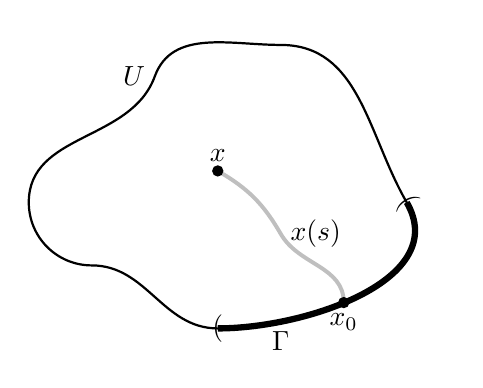
\begin{tikzpicture}[scale=.8]
					\draw[thick] (0,0) to [out=90,in=250] (2,2) to [out=70,in=180] (4,2.5) to [out=0,in=120] (6,0) to [out=300,in=0] (3,-2) to [out=180,in=0] (1,-1) to [out=180,in=270] (0,0);
					\draw[line width=.8mm] (6,0) to [out=300,in=0] (3,-2) node {(};
					\draw[line width=.5mm,gray!50] (5,-1.59) to [out=90,in=300] (4,-.5) to [out=120,in=330] (3,.5);
					\fill (3,.5) circle [radius=.9mm] node [above] {$x$};
					\node at (4,-.5) [right] {$x(s)$};
					\node[rotate=120] at (6,0) {)};
					\node at (4,-2.2) {$\Gamma$};
					\fill (5,-1.59) circle [radius=.9mm];
					\node at (5,-1.9) {$x_0$};
					\node at (2,2) [left] {$U$};
				\end{tikzpicture}
			\end{center}
			We look for an ODE for $u(x(s))$ knowing that $u(x(0))=u(x_0)=g(x_0)$.
			\\

			\noindent \underline{Notation}: $F=F(p_1,\dots,p_n,z,x_1,\dots,x_n)=F(p,z,x)$. We set $\nabla_pF=(\frac{\partial F}{\partial p_1},\dots,\frac{\partial F}{\partial p_n})$, $\nabla_xF=(\frac{\partial F}{\partial x_1},\dots,\frac{\partial F}{\partial x_n})$. The $x(s)$ depicted in the picture is called the characteristic curve.
			\\

			Now let $x(s)=(x^1(s),\dots,x^n(s))$ be a parametrisation of the curve $x:I\rightarrow\R^n$. Assume that $u\in C^1(U)$. Moreover, define
			\begin{enumerate}
				\item[(iii)] $z(s):=u(x(s))$
				\item[(iv)] $p(s):=\nabla u(x(s))$
			\end{enumerate}
			so that $p(s)=(p^1(s),\dots,p^n(s))$ where $p^i(s)=\frac{\partial u}{\partial x_i}(x(s))$ for $i=1,\dots,n$. If we differentiate $p^i$ with respect to $s$ we obtain
			\begin{equation}\label{def p^i}
				\dot{p}^i(s)=\sum_{j=1}^n\frac{\partial^2 u}{\partial x_i\partial x_j}\,x(s)\dot{x}^j(s)
			\end{equation}
			which contains second-order derivatives of $u$. Let us go back to (i) and differentiate it with respect to $x_i$ to get 
			\begin{equation}\label{eq--7}
				\sum_{j=1}^n\frac{\partial F}{\partial p^j}(\nabla u,u,x)\frac{\partial^2 u}{\partial x_i\partial x_j}+\frac{\partial F}{\partial z}(\nabla u,u,x)\frac{\partial u}{\partial x_i}+\frac{\partial F}{\partial x_i}(\nabla u,u,x)=0.
			\end{equation}
			Now make a crucial but \textit{ad hoc} ansatz:
			\begin{equation}\label{eq--8}
				\dot{x}^j(s)=\frac{\partial F}{\partial p^j}(p(s),z(s),x(s)).
			\end{equation}
			If we evaluate \eqref{eq--7} at $x(s)$ we get
			\begin{equation*}
				\sum_{j=1}^n\frac{\partial F}{\partial p^j}(p(s),z(s),x(s))\frac{\partial^2 u}{\partial x_i\partial x_j}(x(s))+\frac{\partial F}{\partial z}(p(s),z(s),x(s))p^i(s)+\frac{\partial F}{\partial x_i}(p(s),z(s),x(s))=0.
			\end{equation*}
			Substituting this and \eqref{eq--8} into \eqref{def p^i} yields
			\begin{equation}\label{eq--9}
				\dot{p}^i(s)=-\frac{\partial F}{\partial z}(p(s),z(s),x(s))p^i(s)-\frac{\partial F}{\partial x_i}(p(s),z(s),x(s)).
			\end{equation}
			Differentiating (iii) with respect to $s$, we find 
			\begin{equation*}
				\dot{z}(s)=\sum_{j=1}^n\frac{\partial u}{\partial x_j}(x(s))\dot{x}^j(s)=\sum_{j=1}^np^j\frac{\partial F}{\partial p^j}(p(s),z(s),x(s)).
			\end{equation*}
			To summarise, we obtain the system of ODEs
			\begin{align}
				\dot{p}(s)&=-\nabla_xF(p(s),z(s),x(s))-D_zF(p(s),z(s),x(s))p(s)\label{eq--start}\\
				\dot{z}(s)&=\nabla_pF(p(s),z(s),x(s))\cdot p(s)\\
				\dot{x}(s)&=\nabla_pF(p(s),z(s),x(s))\label{eq--stop}
			\end{align}
			subject to the initial conditions. This is a system of ODEs with unknown functions $p(s),z(s),x(s)$. Observe that the ansatz made for $\dot{x}$ produces a system of $2n+1$ equations in $2n+1$ unknowns. 

			\begin{defi}
				(Characteristic equations) The system \eqref{eq--start}-\eqref{eq--stop} of ODEs is called the characteristic equations of the PDE $F(\nabla u, u, x)=0$.
			\end{defi}

			\noindent\underline{NB}: We emphasise that the function $F$ defining the PDE can be fully non-linear in $u$ and its derivatives, which makes the fact that it can be solved explicitly so remarkable.

			\begin{eg}
				Consider the (non-linear) equation for $(x_1,x_2)\in U$, where $U$ is the right half-plane and $\Gamma$ its boundary, i.e. the $y$-axis:
				\begin{equation*}
					\begin{cases}
						\del{u}{x_1}\del{u}{x_2}=u & \text{on }U\\
						u(0,x_2)=x_2^2 & \text{on }\Gamma	
					\end{cases}.
				\end{equation*}
				The function $F$ associated to this equation is $F(p,z,x)=p_1p_2-z$. Now use the characteristic equations:
				\begin{equation*}
					\dot{p}_1=p_1,\qquad\dot{p}_2=p_2,\qquad\dot{z}=2p_1p_2,\qquad\dot{x}_1=p_2,\qquad\dot{x}_2=p_1.
				\end{equation*}
				Solving the equations for $p$ is easy: $p_1(s)=p_1^{(0)}\e{s}$ and $p_2(s)=p_2^{(0)}\e{s}$ with $p_{1,2}^{(0)}$ constants. We use these to solve for $z$, $z(s)=z^{(0)}+p_1^{(0)}p_2^{(0)}(\e{2s}-1)$, and also $x$: $x_1(s)=p_2^{(0)}(\e{s}-1)$, $x_2(s)=x_0+p_1^{(0)}(\e{s}-1)$ for $x_0,z^{(0)}\in\R$ constant.\\
				Use the boundary condition to determine $p^{(0)}=(p_1^{(0)},p_2^{(0)})$ and $x_0$ and $z^{(0)}$. Since $u=x_2^2$ on $\Gamma$, we have $p_2^{(0)}=\del{u}{x_2}(0,x_2)=2x_0$. Furthermore, the PDE $\del{u}{x_1}\del{u}{x_2}=u$ implies that $p_1^{(0)}p_2^{(0)}=z^{(0)}=(x_0)^2$ and so $p_1^{(0)}=\frac{x_0}{2}$. Hence, 
				\begin{equation*}
					x_1(s)=2x_0(\e{s}-1),\quad x_2(s)=\frac{x_0}{2}(\e{s}-1),\quad z(s)=x_0^2\e{2s},\quad p_1(s)=\frac{x_0}{2}\e{s},\quad p_2(s)=2x_0\e{s}.
				\end{equation*}
				Fix $(x_1,x_2)\in U$, choose $s,x_0$ so that $(x_1,x_2)=(x_1(s),x_2(s))=(2x_0(\e{s}-1),\frac{x_0}{2}(\e{s}+1))$. This implies $x_0=\frac{4x_2-x_1}{4}$ and $\e{s}=\frac{x_1+4x_2}{4x_2-x_1}$. So
				\begin{equation*}
					u(x_1,x_2)=u(x_1(s),x_2(s))=z(s)=\left(\frac{4x_2-x_1}{4}\right)^2\left(\frac{x_1+4x_2}{4x_2-x_1}\right)^2=\frac{(x_1+4x_2)^2}{16}.
				\end{equation*}
			\end{eg}


		% \section{Linear Partial Differential Operators}
		\section{Linear Partial Differential Operators}

			\begin{defi}
				(Multi-index) A multi-index $\alpha=(\alpha_1,\dots,\alpha_n)$ is an $n$-tuple of non-negative integers $\alpha_i\in\N$. Moreover, we define
				\begin{enumerate}
					\item the length of $\alpha$ given by $|\alpha|=\sum_{i=1}^n\alpha_i$,
					\item the factorial $\alpha!=(\alpha_1!)(\alpha_2!)\dots(\alpha_n!)$,
					\item for $x\in\R^n$, $x=(x_1,\dots,x_n)$: $x^\alpha=x_1^{\alpha_1}x_2^{\alpha_2}\dots x_n^{\alpha_n}$,
					\item differentiation $\partial^\alpha=\del[|\alpha|]{}{x_1^{\alpha_1}\partial x_2^{\alpha_2}\dots\partial x_n^{\alpha_n}}$.
				\end{enumerate}
			\end{defi}

			\begin{eg}
				Let $\alpha=(1,0,3)$. Then $|\alpha|=1+0+3=4$ and for $x\in\R^3$, $x^\alpha=x_1x_3^3$, $\partial^\alpha=\partial_1\partial_3^3$.
			\end{eg}

			\begin{defi}
				A general linear partial differential operator (PDO) of order $m$ is a linear operator of the form
				\begin{equation*}
					P(x,\partial)=\sum_{|\alpha|\le m}a_\alpha(x)\partial^\alpha.
				\end{equation*}
			\end{defi}

			\noindent\underline{NB}: $P$ is said to be linear since for functions $f,g$ and real numbers $\alpha$ and $\beta$ one has $$P(x,\partial)(\alpha f(x)+ \beta g(x))=\alpha P(x,\partial)f(x)+ \beta P(x,\partial)g(x).$$

			\begin{eg}
				Let $x\in\R^2$ and $\alpha=(\alpha_1,\alpha_2)$. Then
				\begin{equation*}
					\sum_{|\alpha|\le 1}a_\alpha(x)\partial^\alpha u(x)=a_{(0,0)}(x)u(x)+a_{(0,1)}(x)\partial_2u(x)+a_{(1,0)}(x)\partial_1u(x).
				\end{equation*}
			\end{eg}

			
			\subsection{Principal Symbol and Characteristic Surfaces}

				\begin{defi}
					(Principal symbol) Associated to $P(x,\partial)$ as in the definition above is the so-called principal symbol of $P$, given by the polynomial 
					\begin{equation*}
						P_m(x,\xi)=\sum_{|\alpha|=m}a_\alpha(x)\xi^\alpha,
					\end{equation*}
					where $\xi\in\R^n$ (or, more precisely, in the tangent space at $x$, $T_x\R^n\simeq\R^n$).
				\end{defi}

				\begin{eg}
					\begin{enumerate}
						\item \textit{Laplacian}: Let $P(x,\partial)=\Delta_{\R^n}$, then $P_2(x,\xi)=|\xi|^2$.
						\item \textit{D'Alembertian}: Let $P(x,\partial)=\del[2]{}{t^2}-\Delta_{\R^n}$, then $P_2(x,\xi)=\tau^2-|\xi|^2$ with $\xi\in\R^n$, $\tau\in\R$. 
						\item \textit{Heat equation operator}: Let $P(x,\partial)=\del[]{}{t}-\Delta_{\R^n}$, then $P_2(x,\xi)=|\xi|^2$ (only highest order derivatives manifest themselves in the principal symbol).
					\end{enumerate}
				\end{eg}

				\begin{defi} (Characteristic surface)
					Let $S$ be a \qt{smooth} hypersurface in $\R^n$ and let $x_0\in S$ be a point on $S$ (smooth in quotation here since we do allow for some singularities). $S$ is said to be characteristic at $x_0$ with respect to $P(x,\partial)$ if a vector $n_{x_0}$ normal to $S$ at $x_0$ satisfies the equality
					\begin{equation*}
						P_m(x_0,n_{x_0})=0.
					\end{equation*}
					A surface is a characteristic surface of a linear partial differential operator $P(x,\partial)$ if it is characteristic with respect to $P$ at all of its points.
				\end{defi}

				\begin{eg}
					Consider
					\begin{equation*}
						P(x,\partial)=\del[2]{}{x_1^2}+\sin(x_1x_2)\del[2]{}{x_2^2}-x_2^2\del[]{}{x_1}\del[]{}{x_2}+x_1\del[]{}{x_1}+\e{x_2}.	
					\end{equation*}
					The principal symbol is given
					\begin{equation*}
						P_2(x_1,x_2,\xi_1,\xi_2)=\xi^2+\sin(x_1x_2)\xi_2^2-x_2^2\xi_1\xi_2.
					\end{equation*}
					Claim: The line $x_2=\frac{\pi}{2}$ is characteristic with respect to $P(x,\partial)$ at the point $x_0=(2,\frac{\pi}{2})$. The normal vector to $S$ at $x_0$ is the vector $(0,1)$. Now we insert into the principal symbol:
					\begin{equation*}
						P_2(2,\frac{\pi}{2},0,1)=0^2+\sin(2\cdot\frac{\pi}{2})\cdot1^2-(\frac{\pi}{2})^2\cdot1\cdot0=0
					\end{equation*}
					as advertised.
				\end{eg}

				\begin{eg}
					Consider
					\begin{equation*}
						P(x,\partial)=\del[2]{}{x_1^2}+\del[2]{}{x_2^2}-\del[2]{}{x_3^2}
					\end{equation*}
					with principal symbol
					\begin{equation*}
						P_2(x,\xi)=\xi_1^2+\xi_2^2-\xi_3^2.
					\end{equation*}
					Claim: The plane given by $x_1+x_2+\sqrt{2}x_3=0$ is a characteristic surface for $P(x,\partial)$. The normal vector is $n_x=(1,1,\sqrt{2})$. Then we find
					\begin{equation*}
						P_2(x,\xi)=1^2+1^2-2=0.
					\end{equation*}
				\end{eg}

				Why would we care about characteristic surfaces? Consider the initial value problem in $\R^2$ with coordinates $(x,y)\in\R^2$:
				\begin{equation*}
					\del[]{u}{x}=0,\qquad u(x,0)=f(x)
				\end{equation*}
				with $f$ some given function. We can rewrite the boundary condition as $u|_S=f$ where $S=\{(x,y)\in\R^2|y=0\}$. The principal symbol is
				$P_1(x,y,\xi_1,\xi_2)=\xi_1$ and the normal at any point in $S$ is $(0,1)$. Hence, $P_1(x,y,0,1)=0$, i.e. $S$ is characteristic for the operator $\del[]{}{x}$. We conclude from the initial value problem that $u(x,y)=\phi(y)$ and hence $u(x,0)=\phi(0)$. Now let $f(x)=x$, then the initial value problem cannot be solved! The problem stems from the fact that $S$ is characteristic.
				Let us now consider the initial value problem
					\begin{equation*}
					\del[]{u}{x}=0,\qquad u(0,y)=f(y)
				\end{equation*}
				
	            Here $S=\{(x,y)\in\R^2|x=0\}$, with normal $n=(1,0)$, we find $P_1(x,y,n)=1\neq0$, i.e. $S$ is not characteristic. Now $u(x,y)=\phi(y)$ with boundary condition $u(0,y)=\phi(y)=f(y)$, which has the unique solution $u(x,y)= f(y)$.

				We extrapolate from this observation that in order to obtain unique solutions of PDEs we should choose as our initial data (initial surfaces) those that are not characteristic with respect to our PDO.



			\subsection{Classification of Second-order PDEs}

				Consider a second-order PDE of the form
				\begin{equation}\label{eq--2ndorder}
					\sum_{i,j}a_{ij}(x)\del[2]{u}{x_i\partial x_j}+\Phi(x,u,\nabla u)=0
				\end{equation}
				where $a_{ij}(x)$ and $\Phi$ are given functions. In general, an equation of this type is called quasi-linear. It is called linear if and only if $\Phi$ is linear in $u$ (and its derivatives, of course).

				Assume that $a_{ij}(x)=a_{ji}(x)$. The goal is to find a linear change of coordinates so to simplify the equation above. Let $M$ be a non-singular matrix and set $y=Mx$. Note that $u(x)=u(M^{-1}y)$. Applying the chain rule we get
				\begin{equation*}
					\del[]{u}{x_i}=\sum_{j=1}^n\del[]{y_k}{x_i}\del[]{u}{y_k}
				\end{equation*}
				and for the second derivatives,
				\begin{equation*}
					\del[2]{u}{x_i\partial x_j}=\sum_{k,l}M_{ki}M_{lj}\del[2]{u}{y_k\partial y_l}.
				\end{equation*}
				Hence, in the new coordinates we get
				\begin{equation*}
					\sum_{i,j}a_{ij}(x)\del[2]{u}{x_i\partial x_j}=\sum_{i,j}a_{ij}(x)\left(\sum_{k,l}M_{ki}M_{lj}\del[2]{u}{y_k\partial y_l}\right)=\sum_{k,l}\left(\sum_{i,j}a_{ij}(x)M_{ki}M_{lj}\right)\del[2]{u}{y_k\partial y_l}
				\end{equation*}
				and we define $b=MaM^T$. 
				This transforms \eqref{eq--2ndorder} into the equation
				\begin{equation*}
					\sum_{k,l}b_{kl}(y)\del[2]{u}{y_k\partial y_l}+\Psi(y,u,\nabla u).
				\end{equation*}
				Now fix $x_0$ and try to find a matrix $M$ such that the matrix $b$ at point $y_0=Mx_0$ is as simple as possible. To do this, set $a_{ij}=a_{ij}(x_0)$ and consider the following quadratic form
				\begin{equation*}
					\sum_{i,j}a_{ij}\xi_i\xi_j=\xi a\xi^T=Q,
				\end{equation*}
				where we set $\xi=(\xi_1,\dots,\xi_n)$. This is the characteristic form of our PDE at $x_0$. Recall that the signature of $Q$ is the pair $(p,q)$ where $p$ is the number of eigenvalue 1 and $q$ the number of eigenvalue -1 in the diagonalisation of $Q$.

				\begin{defi}
					(Types of second-order PDEs) A second-order PDE of the form \eqref{eq--2ndorder} in $n$ dimensions is
					\begin{enumerate}
						\item of elliptic type at $x_0$ if its associated quadratic form $Q$ has signature $(p,q)=(0,n)$ or $(p,q)=(n,0)$,
						\item of hyperbolic type at $x_0$ if $Q$ has signature $(p,q)=(n-1,1)$ or $(p,q)=(1,n-1)$,
						\item of parabolic type at $x_0$ if $Q$ has signature $(p,q)=(n-1,0)$ or $(p,q)=(0,n-1)$.
					\end{enumerate}
				\end{defi}

				\begin{eg}
					\begin{enumerate}
						\item The quadratic form associated to $\Delta_{\R^n}$ has the matrix $I_{n\times n}$ at every point. Therefore, $\Delta_{\R^n}$ is elliptic.
						\item For the wave operator $\del[2]{}{t^2}-\Delta_{\R^n}$ in $\R^{n+1}$, the signature is $(1,n)$. Therefore, the wave operator is hyperbolic.
						\item For the heat operator $\del[]{}{t}-\Delta_{\R^n}$ in $\R^{n+1}$, the signature is $(0,n)$. Therefore, the heat operator is parabolic.
					\end{enumerate}
				\end{eg}

		\section{Distribution Theory}

			\noindent Motivation: From calculus one encounters functions like the Heaviside function (named after English mathematician and physicist Oliver Heaviside) $\mathrm{H}(x)$ or the absolute value function $f(x)=|x|$,
			\begin{center}
				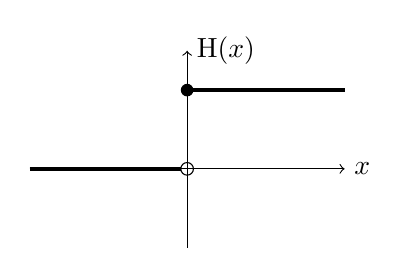
\begin{tikzpicture}[scale=1]
					\draw[->] (-2,0)--(2,0) node [right]{$x$};
					\draw[->] (0,-1)--(0,1.5) node [right]{$\mathrm{H}(x)$};
					\draw[line width=.5mm] (-2,0)--(-.08,0);
					\draw[line width=.5mm] (0,1)--(2,1);
					\draw[] (0,0) circle [radius=.08cm];
					\fill (0,1) circle [radius=.08cm];
				\end{tikzpicture}
				\qquad\qquad
				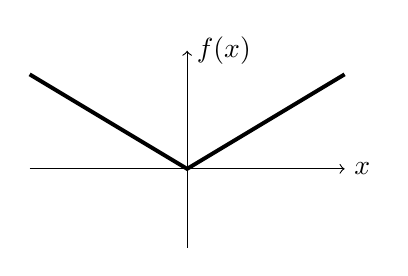
\begin{tikzpicture}[scale=1]
					\draw[->] (-2,0)--(2,0) node [right]{$x$};
					\draw[->] (0,-1)--(0,1.5) node [right]{$f(x)$};
					\draw[line width=.5mm] (-2,1.2)--(0,0)--(2,1.2);
				\end{tikzpicture}
			\end{center}
			$\mathrm{H}(x)$ and $f(x)$ are not differentiable (as functions) at $x=0$.
			\\

			\noindent The British physicist Paul Dirac introduced a \qt{function} in quantum mechanics that was defined as follows:
			\begin{equation*}
				\delta(x)=\begin{cases}
					0, & x\neq0\\
					\delta(x), & x=0
				\end{cases}
			\end{equation*}
			in such a way that $\int_{-\infty}^\infty \delta(x)\mathrm{d}x=1$. Although such a function doesn't really exist (since the definition of $\delta$ would imply that it is zero almost everywhere and hence its integral has to be zero), we shall see that one can interpret $\delta$ as a well-defined distribution.
			\\

			Simplistically, distributions are needed to make sense of derivatives of $|x|$, $\mathrm{H}(x)$ and of the definition of the Dirac delta function, but actually their domain of applications go far beyond that, e.g. the theory of partial differential equations as well as quantum field theory.


		\subsection{Test Functions}

			\begin{defi}(Space of test functions)
				Denote by $C^\infty_c(\R^n)$ or $C_0^\infty(\R^n)$ the space of infinitely differentiable functions on $\R^n$ with compact support $\supp\phi=\overline{\{x\in\R^n|\phi(x)\neq0\}}$.
			\end{defi}

			\begin{eg}
				Bump functions are elements of $C^\infty_c(\R^n)$, e.g.
				\begin{equation*}
					b(x)=\begin{cases}
						\e{-\frac{1}{1-|x|^2}}, & |x|<1\\
						0, & |x|\ge1
					\end{cases}\qquad\qquad
					\begin{tikzpicture}[baseline=.1cm]
						\draw[->] (-2,0)--(2.1,0) node [right]{$x$};
						\draw[->] (0,-1)--(0,1.5) node [right]{$b(x)$};
						\draw[thick](1,-.1)--(1,.1) node [below,yshift=-1.5mm]{1};
						\draw[thick](-1,-.1)--(-1,.1) node [below,yshift=-1.5mm]{-1};
						\draw[line width=.5mm] plot [smooth] file {plots/bump.table};
						\draw[line width=.5mm] plot [smooth] file {plots/bump1.table};
					\end{tikzpicture}
				\end{equation*}
			\end{eg}

			\begin{defi}(Convolution)
				Let $\phi$ be a bounded measurable function and $\psi\in L^1(\R^n)$. Then the convolution (or folding) of $\phi$ and $\psi$ denoted by $\phi\ast\psi(x)$ is defined by
				\begin{equation*}
					\phi\ast\psi(x)=\int_{\R^n}\phi(x-y)\psi(y)\mathrm{d}y.
				\end{equation*}
			\end{defi}

			\begin{prop}\label{prop--convolution}
				Convolution has the following nice properties:
				\begin{enumerate}
					\item $\phi\ast\psi=\psi\ast\phi$,
					\item if $\psi\in L^1(\R^n)$ and $\phi\in C^\infty_c(\R^n)$ and $\del[\alpha]{\phi}{x^\alpha}$, $|\alpha|\le m$ are continuous and bounded, then $\phi\ast\psi$ and $\del[\alpha]{}{x^\alpha}(\phi\ast\psi)$ are also continuous and bounded.
				\end{enumerate}
			\end{prop}
			\begin{proof}
				Property (i) follows from substitution $y\mapsto x-y$ and then (ii) follows from (i) using that $\phi$ is smooth.
			\end{proof}

			\begin{prop}
				Let $\phi$ and $\psi$ be continuous functions with compact support, $\supp\phi\subset U_1$ and $\supp\psi\subset U_2$ with $U_{1},U_2\subset\R^n$ open. Then
				\begin{equation*}
					\supp(\phi\ast\psi)\subset U_1+U_2=\{x+y\in\R^n|x\in U_1, y\in U_2\}.
				\end{equation*}
			\end{prop}
			\begin{pproof}
				Exercise.
			\end{pproof}
			
			\begin{prop}\label{prop--approx}
				(Approximation by $C^\infty_c$ functions) The space $C^\infty_c$ is dense in the space $C_c(\R^n)$ (the space of continuous functions with compact support). This means that for any continuous function $\phi$ with support in $B(0,R)=\{x\in\R^n|\,|x|< R\}$ there exists a sequence of $C^\infty_c$-functions $\phi_m$ with support in $B(0,R)$ such that $\lim_{m\rightarrow\infty}\max_{x\in\R^n}|\phi_m(x)-\phi(x)|=0$.
			\end{prop}
			\begin{proof}
				First, consider the function 
				\begin{equation*}
					\chi(x)=\begin{cases}
						\e{-\frac{1}{1-|x|^2}}, & |x|<1\\
						0, & |x|\ge1
					\end{cases}.
				\end{equation*}
				Clearly $\chi\in C^\infty_c(\R^n)$ and is supported in $B(0,1)$. Now, let $c_n=\int_{\R^n}\chi(x)\mathrm{d}x$. Set $\chi_\delta(x):=\frac{1}{c_n\delta^n}\chi(\frac{x}{\delta})\ge0$ for $\delta>0$ and
				\begin{equation*}
					\int_{\R^n}\chi_\delta(x)\mathrm{d}x=\frac{1}{c_n\delta^n}\int_{\R^n}\chi\left(\frac{x}{\delta}\right)\mathrm{d}x=\frac{1}{c_n}\int_{\R^n}\chi(y)\mathrm{d}y=1.
				\end{equation*}
				Note that $\chi_\delta$ is supported in $B(0,\delta)$. Given a continuous function $\phi$ with $\supp\phi\subset B(0,R)$, define $\phi_\delta(x):=\phi\ast\chi_\delta(x)$. Since $\supp\phi$ is closed and $B(0,R)$ is open there exists $R_1<R$ such that $\supp\phi\subset B(0,R_1)$. If $0<\delta< R-R_1$ then $\supp\phi_\delta\subset B(0,R)$ since $\supp\chi_\delta\subset B(0,\delta)$ and $B(0,R_1)+B(0,\delta)\subset B(0,R)$. Also, from \autoref{prop--convolution} (ii) we get $\phi_\delta$ smooth, i.e. $\phi_\delta\in C^\infty_c(\R^n)$. Now it remains to show that $\phi_\delta(x)$ converges uniformly to $\phi(x)$ as $\delta\rightarrow0$. We have 
				\begin{align*}
					|\phi_\delta(x)-\phi(x)|&=\left|\int_{\R^n}\phi(x-y)\chi_\delta(y)\mathrm{d}y-\phi(x)\int_{\R^n}\chi_\delta(y)\mathrm{d}y\right|\\
					&=\left|\int_{\R^n}(\phi(x-y)-\phi(x))\chi_\delta(y)\mathrm{d}y\right|\\
					&=\int_{|y|\le\delta}|\phi(x-y)-\phi(x)|\chi_\delta(y)\mathrm{d}y.
				\end{align*}
				Since $\phi$ is uniformly continuous for any $\epsilon>0$ there is $\delta_0$ such that $|\phi(x-y)-\phi(x)|<\epsilon$ for all $x\in\R^n$ and $|y|<\delta_0$. Thus we get
				\begin{equation*}
					|\phi_\delta(x)-\phi(x)|<\epsilon\int_{|y|<\delta}\chi_\delta(y)\mathrm{d}y=\epsilon
				\end{equation*} 
				if $\delta<\delta_0$.
			\end{proof}


		\subsection{Mollifiers}

			\noindent Idea: Starting out with a bad-behaved function turn it into a nice function, \qt{mollify} it. This is precisely what we did in the proof of \autoref{prop--approx}.
			\\

			\noindent To start, consider again the function
			\begin{equation*}
				\chi(x)=\begin{cases}
					c_n\e{\frac{1}{|x|^2-1}}, & |x|<1\\
					0, & |x|\ge1
				\end{cases}.
			\end{equation*}
			Choose $c_n$ such that $\int_{\R^n}\chi(x)\mathrm{d}x=1$. Then consider the convolution $u_\delta(x)=u\ast\chi_\delta(x)$ with $\chi_\delta(x)=\frac{1}{\delta^n}\chi(\frac{x}{\delta})$ ($\delta>0$) and $u$ some function. Now suppose $\Omega$ is an open subset of $\R^n$, $u\in L^p(\Omega)$ with $1\le p$. Then $u\in L^1_\mathrm{loc}(\Omega)$, so for $\delta>0$, as long as $\dist(x,\partial\Omega)>\delta$, $u_\delta(x)$ is well-defined. Furthermore, for any $\Omega^\prime$ such that $\bar{\Omega^\prime}\subset\Omega$ with $\dist(\Omega^\prime,\partial\Omega)>\delta$, we have $u_\delta\in C^\infty(\Omega^\prime)$. Also, if $u\in L^p(\R^n)$ and $u$ has compact support in $\R^n$, then $u_\delta\in C^\infty_c(\R^n)$.
			
			\begin{defi}
				(Mollification) The function $u_\delta$ defined above is called the mollification of $u$ and $\chi_\delta$ is called the (Friedrichs) mollifier (after German mathematician Kurt Friedrichs).
			\end{defi}

			Recall that if $u\in C_c(\R^n)$, then we showed that $u_\delta(x)$ converges uniformly to $u$ as $\delta\rightarrow0$.

			\begin{lemma}
				For $u\in L^p(\Omega)$, $1\le p<\infty$, $\lim_{\delta\to 0}\norm{u_\delta-u}_{L^p(\Omega)}=0$ with $u_\delta\in C^\infty(\Omega)$.
			\end{lemma}
			\begin{proof}
				In the case $\Omega\neq\R^n$, we extend $u$ trivially by setting $u=0$ outside $\Omega$. Then $u\in L^p(\R^n)$ and since $\norm{u_\delta-u}_{L^p(\Omega)}\le\norm{u_\delta-u}_{L^p(\R^n)}$, it is enough to show the convergence in $\R^n$. Now,
				\begin{align*}
					\norm{u_\delta-u}_{L^p(\R^n)}=&\left(\int\left|\int(u(x-\delta y)-u(x))\chi(y)\mathrm{d}y\right|^p \mathrm{d}x\right)^{\frac{1}{p}}\\
					=&\norm{\int(u(x-\delta y)-u(x))\chi(y)\mathrm{d}y}_{L^p_x(\R^n)}\\
					\le&\int\norm{u(x-\delta y)-u(x)}_{L^p_x(\R^n)}|\chi(y)|\mathrm{d}y\\
					\le&\sup_{|y|\le 1}\norm{u(x-\delta y)-u(x)}_{L^p_x}\int|\chi(y)|\mathrm{d}y\\
					\le& C\sup_{|y|\le1}\norm{u(x-\delta y)-u(x)}_{L^p_x(\R^n)},
				\end{align*}
				where for the first inequality we used Minkowski's inequality.
				Now let $\delta\to 0$ and use the fact from Lebesgue integration theory that $\lim_{h\to0}\norm{u(\cdot+h)-u(\cdot)}_{L^p}=0$ for all $u\in L^p(\R^n)$ and $1\le p<\infty$.
			\end{proof}


		\subsection{Topology on $C^\infty_c(\R^n)$}

			We call $\D(\R^n)$ the space of all $C^\infty_c$-functions with the following notion of convergence (i.e. topology):

			\begin{defi}\label{def--convergence}
				(Convergence) A sequence $\phi_m\in C^\infty_c(\R^n)$ converges to $\phi\in C^\infty_c(\R^n)$ in $\D(\R^n)$ if
				\begin{enumerate}
					\item $\exists R>0,\forall m:\supp\phi_m\subset B(0,R)$,
					\item $\sup_{x\in\R^n}|\phi_m(x)-\phi(x)|$ and $\sup|\del[\alpha]{\phi_m(x)}{x^\alpha}-\del[\alpha]{\phi(x)}{x^\alpha}|$ both approach zero as $m\to\infty$ for all multi-indices $\alpha$.
				\end{enumerate}
			\end{defi}

			\begin{eg}
				Take $\phi_m(x)=\e{-m}\chi(x)\sin(mx)\in C^\infty_c(\R)$ with $\chi$ the usual bump function. Then $\supp\phi_m(x)\subset B(0,1)=(-1,1)$ for all $m$ and $|\del[k]{\phi_m}{x^k}|\le c_k\e{-m}m^k$ (all derivatives hitting the sine function). Thus, we get $\phi_m(x)\to0$ as $m\to\infty$ in $\D(\R)$.	
			\end{eg}

			\begin{eg}
				The function $\phi_m(x)=\frac{1}{m}\chi(\frac{x}{m})$ does not converge to 0 in $\D$. Note that $|\del[\alpha]{\phi_m(x)}{x^\alpha}|\le\frac{c_{|\alpha|}}{m^{|\alpha|+1}}$, i.e. $\del[\alpha]{\phi_m}{x^\alpha}\to0$ uniformly (RHS is independent of $x$). However, we have $\supp\phi_m=\overline{B(0,m)}$, i.e. condition (i) from \autoref{def--convergence} is violated.
			\end{eg}

			\begin{defi}
				(Distribution, defined by the French mathematician Laurent Schwartz, who was awarded a Fields medal 1950 for distribution theory) A linear continuous functional $f$ on $\D$ is called a distribution. Thus, $f:\D\rightarrow\CC$ is a distribution if the following conditions are satisfied:
				\begin{enumerate}
					\item (Linearity) $\forall\alpha_1,\alpha_2\in\CC, \forall\phi_1,\phi_2\in\D:f(\alpha_1\phi_1+\alpha_2\phi_2)=\alpha_1f(\phi_1)+\alpha_2f(\phi_2)$
					\item (Continuity) If $\lim_{m\to\infty}\phi_m=0$ in $\D$, then $\lim_{m\to\infty}f(\phi_m)=0$.
				\end{enumerate}
			\end{defi}

			\noindent\underline{NB}: While the notion of convergence in $\D$ as defined in \autoref{def--convergence} is fairly strong, after applying the functional, the resulting sequence is just a sequence in $\CC$, i.e. the usual (much simpler) definition of convergence applies.
			
			\begin{eg}(Dirac distribution)
				Define the functional $\delta_a$ for $a\in\R^n$ as $\delta_a(\phi):=\phi(a)$ for $\phi\in\D(\R^n)$. We want to show that $\delta_a$ is indeed a distribution. First, we check linearity:
				\begin{equation*}
					\delta_a(\alpha_1\phi_1+ \alpha_2\phi_2)=\alpha_1\phi_1(a)+\alpha_2\phi_2(a)=\alpha_1\delta_a(\phi_1)+ \alpha_2\delta_a(\phi_2).
				\end{equation*}
				Now for continuity: take a sequence $(\phi_m)_m\subset\D$ such that $\phi_m\to0$ in $\D$. Then $\delta_a(\phi_m)=\phi_m(a)$ and so $\lim_{m\to\infty}\delta_a(\phi_m)=0$. This distribution is called the Dirac delta distribution (or Dirac measure) supported at the point $a$.
			\end{eg}

			In functional analysis for a space $V$, the space of linear continuous functionals on $V$ is called the dual space of $V$ and is denoted by $V^\prime$ (or $V^\ast,V^\vee$). Hence, we denote the space of distributions as $\D^\prime(\R^n)$.

			\begin{eg}
				If $f\in L^1_\mathrm{loc}(\R^n)$ then $f$ can be identified with an element of $\D^\prime(\R^n)$ through 
				\begin{equation*}
					f(\phi):=\int_{\R^n}f(x)\phi(x)\mathrm{d}x.
				\end{equation*}
				Linearity is immediate. For continuity, if $(\phi_m)_m\subset\D$ with $\phi_m\to0$ as $m\to\infty$, then it follows that
				\begin{equation*}
					\left|\int_{\R^n}f(x)\phi_m(x)\mathrm{d}x\right|\le\sup_{|x|<R}\int_{|x|<R}|f(x)|\mathrm{d}x
				\end{equation*}
				using (i) of \autoref{def--convergence} and $f$ locally integrable. Since $\phi_m\to0$ in $\D$ we know that $\sup_{|x|<R}|\phi_m(x)|\to0$ as $m\to\infty$.
			\end{eg}

			Now let us revisit the earlier definitions for the case of a domain $\Omega\subset\R^n$.

			\begin{defi}
				(Distributions on a domain) Let $\Omega$ be an arbitrary domain. The space $\D(\Omega)$ is the space $C^\infty_c(\Omega)$ with the following convergence: $\phi_n\in C^\infty_c(\Omega)$ converges to $\phi\in C^\infty_c(\Omega)$ if
				\begin{enumerate}
					\item there exists a subdomain $M$ with $\bar{M}\subset\Omega$ such that $\supp\phi_n\subset\bar{M}$ for all $n$,
					\item $\partial^\alpha\phi_n(x)$ converges uniformly on $\bar{M}$ to $\partial^\alpha\phi(x)$ for all $\alpha$.
				\end{enumerate}
				The space of distributions $\D^\prime(\Omega)$ is the space of all continuous linear functionals on $\D(\Omega)$.
			\end{defi}

			\begin{eg}
				Let $f(x)=\e{x^{-2}}$ and define for all $\phi\in C^\infty_c(0,\infty)$ 
				\begin{equation*}
					f(\phi)=\int_0^\infty\e{x^{-2}}\phi(x)\mathrm{d}x\qquad\qquad
					\begin{tikzpicture}[baseline=.1cm]
						\draw[->] (-2,0)--(2.1,0) node [right]{$x$};
						\draw[->] (-1.5,-1)--(-1.5,1.5) node [right]{$\phi(x)$};
						\draw[line width=.5mm] plot [smooth] file {plots/bump.table};
						\draw[line width=.5mm] plot [smooth] file {plots/bump1.table};
					\end{tikzpicture}
				\end{equation*}
				This yields a distribution in $\D(0,\infty)$.
			\end{eg}

		
		\subsection{Operations on Distributions}

			\begin{defi}
				(Differentiation of a distribution) Let $f\in\D^\prime$. Then, given multi-index $\alpha$ and $\phi\in C^\infty_c$, one has 
				\begin{equation*}
					\partial^\alpha f(\phi):=(-1)^{|\alpha|}f(\partial^\alpha\phi).
				\end{equation*}
			\end{defi}

			\noindent\underline{NB}: The intuition behind the definition above is through integration by parts: 
			\begin{equation*}
				f^\prime(\phi)=\int_{-\infty}^\infty f^\prime(x)\phi(x)\mathrm{d}x=\left[f\phi\right]^\infty_{-\infty}-\int_{-\infty}^\infty f(x)\phi^\prime(x)\mathrm{d}x=-\int_{-\infty}^\infty f(x)\phi^\prime(x)\mathrm{d}x=-f(\phi^\prime)
			\end{equation*}
			where we used compact support of $\phi$ for the third equality.

			\begin{eg}
				(Heaviside function) Consider the Heaviside function
				\begin{equation*}
					\mathrm{H}(x)=\begin{cases}
						1, & x\ge0\\
						0, & x<0
					\end{cases}\qquad\qquad 
					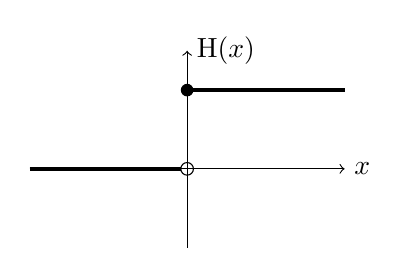
\begin{tikzpicture}[baseline=.1cm]
						\draw[->] (-2,0)--(2,0) node [right]{$x$};
						\draw[->] (0,-1)--(0,1.5) node [right]{$\mathrm{H}(x)$};
						\draw[line width=.5mm] (-2,0)--(-.08,0);
						\draw[line width=.5mm] (0,1)--(2,1);
						\draw[] (0,0) circle [radius=.08cm];
						\fill (0,1) circle [radius=.08cm];
					\end{tikzpicture}
				\end{equation*}
				Take $\phi\in C^\infty_c(\R)$ and compute
				\begin{equation*}
					\mathrm{H}^\prime(\phi)=(-1)\mathrm{H}(\phi^\prime)=-\int_{-\infty}^{\infty}\mathrm{H}(x)\phi^\prime(x)\mathrm{d}x=-\int_{-\infty}^\infty\phi^\prime(x)\mathrm{d}x=\phi(0)=\delta_0(\phi)	
				\end{equation*}
				where we used compact support of $\phi$. We conclude $\mathrm{H}^\prime=\delta_0$ (the Dirac functional).
			\end{eg}

			\begin{eg}
				Consider the function $f(x)=|x|$. What is $f^\prime(x)$? On the level of the functional we find
				\begin{align*}
					f^\prime(\phi)=&-f(\phi^\prime)=-\int_{-\infty}^\infty|x|\phi^\prime(x)\mathrm{d}x=\int_{-\infty}^0x\phi^\prime(x)\mathrm{d}x-\int_0^\infty x\phi^\prime(x)\mathrm{d}x\\=&[x\phi(x)]_{-\infty}^0-\int_{-\infty}^0\phi(x)\mathrm{d}x-[x\phi(x)]_0^\infty+\int_0^\infty\phi(x)\mathrm{d}x=\int_0^\infty\phi(x)\mathrm{d}x-\int_{-\infty}^0\phi(x)\mathrm{d}x.
				\end{align*}
				Define the sign function as follows:
				\begin{equation*}
					\sn x=\begin{cases}
						1, & x>0\\
						0, & x=0\\
						-1, & x<0
					\end{cases}.
				\end{equation*}
				Then $f^\prime(\phi)=\int\sn(x)\phi(x)\mathrm{d}x=\sn(\phi)$, i.e. $|x|^\prime=\sn(x)$.
			\end{eg}

			\begin{defi}
				(Multiplication with smooth functions) If $a\in C^\infty$ and $f\in\D^\prime$, then $af\in\D^\prime$ and for all $\phi\in C^\infty_c$, $af(\phi)=f(a\phi)$.
			\end{defi}

			\noindent\underline{NB}: One can not, in general, multiply two distributions (naive definitions thereof would not be associative).


		\subsection{Convergence of Sequences of Distributions}

			\begin{defi}
				We say that the sequence $f_n\in\D^\prime$ converges to a distribution $f\in\D^\prime$ if $\lim_{n\to\infty}f_n(\phi)=f(\phi)$ for all $\phi\in C^\infty_c$.
			\end{defi}

			\begin{eg}
				(Delta sequences)
				\begin{enumerate}
					\item Let $\beta(x)\ge0$ on $x\in\R^n$ and $\int_{\R^n}\beta(x)\mathrm{d}x=1$. Let $\beta_\epsilon(x):=\frac{1}{\epsilon^n}\beta(\frac{x}{\epsilon})$. Then $\beta_\epsilon\to\delta_0$ as $\epsilon\to 0$ in $\D^\prime$.
					To see this we take an arbitrary test function $\phi\in\D$ and look at
					\begin{align*}
						\beta_\epsilon(\phi)-\delta_0(\phi)=&\beta_\epsilon(\phi)-\phi(0)=\int_{\R}\beta_\epsilon(x)\phi(x)\mathrm{d}x-\phi(0)=\int_{\R^n}\beta(y)\phi(\epsilon y)\mathrm{d}y-\phi(0)\\
						=&\int_{\R^n}\beta(y)(\phi(\epsilon y)-\phi(0))\mathrm{d}y.
					\end{align*} 
					Since $|\phi(\epsilon y)-\phi(0)|\le C$ for some positive constant $C$ and $\phi(\epsilon y)\to\phi(0)$ as $\epsilon\to 0$ we obtain, by Lebesgue's dominated convergence theorem, that
					\begin{equation*}
						\left|\int_{\R^n}\beta(y)(\phi(\epsilon y)-\phi(0))\mathrm{d}y\right|\le\int_{\R^n}\beta(y)|\phi(\epsilon y)-\phi(0)|\mathrm{d}y\underset{\epsilon\to0}{\longrightarrow}0
					\end{equation*}
					\item The Poisson kernel for the Laplace equation in two dimensions is
					\begin{equation*}
						p(x_1,x_2):=\frac{x_2}{\pi(x_1^2+x_2^2)}.
					\end{equation*} 
					Note that if $x_2>0$ (i.e. we are in the upper half plane) then $\del[2]{p}{x_1^2}+\del[2]{p}{x_2^2}=0$. Define $\beta(x_1):=\frac{1}{\pi(x_1^2+1)}$. Then
					\begin{equation*}
						\int_{\R}\beta(x_1)\mathrm{d}x=\frac{1}{\pi}\int_\R\frac{\mathrm{d}x_1}{1+x_1^2}=1.
					\end{equation*}
					Note that $p(x_1,x_2)=\frac{1}{x_2}\beta(\frac{x_1}{x_2})$. Therefore by the previous result, $p(x_1,x_2)\to\delta_0$ as $x_2\to0$.
					\item The heat kernel in $\R^n$ is given by
					\begin{equation*}
						H(x,t)=\frac{1}{(4\pi t)^{\frac{n}{2}}}\e{-\frac{|x|^2}{4t}}.
					\end{equation*} 
					$H$ satisfies the heat equation $\del[]{H}{t}-\Delta_x H=0$, $t>0$. Note that $\frac{1}{\pi^{\frac{n}{2}}}\int_{\R^n}\e{-|x|^2}\mathrm{d}x=1$ so take $\beta(x):=\frac{1}{\pi^{\frac{n}{2}}}\e{-|x|^2}$. Then $H(x,t)=\frac{1}{(4t)^{\frac{n}{2}}}\beta(\frac{x}{2\sqrt{t}})$. Since $(4t)^{\frac{n}{2}}=(2\sqrt{t})^n$, we take $\epsilon=2\sqrt{t}$. Therefore, as $t\to0^+$, $H(x,t)\to\delta_0$ in $\D^\prime$.
				\end{enumerate}
			\end{eg}



	\section{Fourier Theory}

		The class $\D^\prime$ is not good enough for the purpose of Fourier transformations. The first step in that direction is hence to define a new class of functions, the Schwartz class.

		\subsection{Schwartz Class $\s$}

			We would like to define the Fourier transform of a distribution $f$ similar to the way we have defined derivatives, i.e. $\hat{f}(\phi)=f(\hat{\phi})$. However, it turns out that $\phi\in C^\infty_c$ are not the appropriate kind of test functions for this purpose. Schwartz produced a new class of test functions with very nice properties regarding the Fourier transform.

			\begin{defi}
				(Schwartz class) Let $\phi\in C^\infty(\R^n)$ such that for all multi-indices $\alpha,\beta$ we have 
				\begin{equation*}
					\sup_{x\in\R^n}|x^\alpha\partial^\beta\phi(x)|<\infty.
				\end{equation*}
				This means that $\phi$ and all its derivatives decay faster than any reciprocal of a polynomial: $|\partial^\alpha\phi(x)|\le c_N(1+|x|)^{-N}$ for all $N\ge1$. This class is denoted by $\s(\R^n)$ (where $\s$ stands for ``spherical'' and not Schwartz, referring to the fact that on a sphere of radius $R$ the function decays rapidly as the radius goes to infinity).
			\end{defi}
	
			\begin{eg}
				A prototypical example of a Schwartz function is the Gaussian
				\begin{equation*}
					f(x)=\e{-|x|^2}\qquad\qquad
					\begin{tikzpicture}[baseline=.1cm]
						\draw[->] (-2,0)--(2.1,0) node [right]{$x$};
						\draw[->] (0,-1)--(0,1.5) node [right]{$f(x)$};
						\draw[line width=.5mm] plot [smooth] file {plots/gauss.table};
					\end{tikzpicture}
				\end{equation*}
			\end{eg}

			
			\begin{remark}
				One might ask why $C^\infty_c$ is not good enough for the purpose of Fourier transformations, despite being an already very nice set of functions. The problem is that if $\phi\in C^\infty_c(\R^n)$ then
				\begin{equation*}
					\hat{\phi}(\xi):=\int_{\R^n}\phi(x)\e{-\i x\cdot\xi}\mathrm{d}x\notin C^\infty_c(\R^n).
				\end{equation*}
				This is due to one of the (many) versions of the Heisenberg uncertainty principle. Hence, we cannot establish a bijective relation between the set of test functions and their Fourier transforms. However, if $\phi\in\s(\R^n)$ then $\hat{\phi}\in\s(\R^n)$. Thus, one can build a theory of distributions that is based on test functions in $\s$.
			\end{remark}

			\begin{defi}
				(Topology of $\s$) Given a sequence $\phi_n\in\s$ we say that $\phi_n\to\phi$ as $n\to\infty$ in $\s$ if for all $N>0$ one has
				\begin{equation*}
					\sup_{x\in\R^n}(1+|x|)^N\left(\sum_{|\alpha|=0}^N|\partial^\alpha\phi_n(x)-\partial^\alpha\phi(x)|\right)\underset{n\to\infty}{\longrightarrow}0
				\end{equation*}
				for all $N>0$.
			\end{defi}

			\noindent\underline{NB}: Note that if $\phi\in C^\infty_c(\R^n)$ then of course $\phi\in\s$, i.e. we have $\D\subset\s$.


		\subsection{Tempered Distributions}

			\begin{defi}
				(Tempered distribution) The space of continuous linear functionals on $\s$ is called the space of tempered distributions and is denoted by $\s^\prime$. This means that $f\in\s^\prime$ if
				\begin{enumerate}
					\item $\forall\alpha_1,\alpha_2\in\CC,\,\phi_1,\phi_2\in\s$: $f(\alpha_1\phi_1+\alpha_2\phi_2)=\alpha_1f(\phi_1)+\alpha_2f(\phi_2)$
					\item $\phi_n\in\s,\,\phi_n\to0:\,\lim_{n\to\infty}f(\phi_n)=0$
				\end{enumerate}
			\end{defi}

			\begin{eg}
				\begin{enumerate}
					\item The Dirac measure $\delta_a\in\s^\prime$.
					\item If $f\in L^p(\R^n)$, $1\le p\le\infty$, then through the pairing $f(\phi):=\int f(x)\phi(x)\mathrm{d}x$, $\phi\in\s$ one can identify  $f$ with an element of $\s^\prime$ (in particular, $f$ does not even have to be continuous).
				\end{enumerate}
			\end{eg}

			\noindent\underline{NB}: Note that $\s^\prime\subset\D^\prime$. However, locally integrable functions are all in $\D^\prime$ but if we take, e.g., $f(x)=\e{x^2}\in L^1_\mathrm{loc}$, then $f\in\D^\prime$ but $f\notin\s^\prime$ (note that $f\in\s$ is not necessarily compactly supported).
			\\

			\noindent Operations with tempered distributions are the following:
			\begin{enumerate}
				\item Addition and subtraction,
				\item differentiation: $\forall\phi\in\s: \partial^{\alpha} f(\phi)=(-1)^{|\alpha|}f(\partial^\alpha\phi)$,
				\item if $a\in C^\infty$ and $|\partial^\alpha a(x)|\le c_\alpha (1+|x|)^{m_\alpha}$ for some $m_\alpha,c_\alpha$ then if $f\in\s^\prime$: $af\in\s^\prime$ and $af(\phi)=f(a\phi)$.
			\end{enumerate}
			\noindent As a consequence, all monomials $x^\alpha (x\in\R^n$, $\alpha$ multi-index) are in $\s^\prime$.


		\subsection{Fourier Transformations in $\s$}

			\begin{defi}
				Given $\phi\in\s$, its Fourier transform is given by
				\begin{equation*}
					\hat{\phi}(\xi):=\int_{\R^n}\phi(x)\e{-\i x\cdot\xi}\mathrm{d}x.
				\end{equation*}
				Note that the integral is absolutely convergent. Moreover, the map $\phi\mapsto\hat{\phi}$ is an isomorphism in $\s$. The Fourier inversion formula is
				\begin{equation*}
					\phi(x)=\frac{1}{(2\pi)^n}\int_{\R^n}\hat{\phi}(\xi)\e{\i x\cdot\xi}\mathrm{d}\xi.
				\end{equation*}
			\end{defi}

			\begin{prop}\label{prop--fourier}
				(Properties of Fourier transform) Assume that $\phi\in\s$, $\lambda\in\R$ and $h\in\R^n$.
				\begin{enumerate}
					\item $\F(\phi(\cdot -h))=\e{-\i h\cdot\xi}\hat{\phi}(\xi)$
					\item $\F(\e{\i h\cdot x}\phi)=\hat{\phi}(\cdot-h)$
					\item If $\sigma_\lambda\phi(x):=\phi(\lambda x)$ then $\F(\sigma_\lambda\phi)(\xi)=|\lambda|^{-n}\hat{\phi}(\frac{\xi}{\lambda})$.
					\item $\F(\partial^\alpha\phi)(\xi)=\i^{|\alpha|}\xi^\alpha\hat{\phi}(\xi)$
					\item $\F(x^\alpha\phi)(\xi)=\i^{|\alpha|}\partial^\alpha\hat{\phi}(\xi)$
					\item $\phi,\psi\in\s$: $\F(\phi\ast\psi)(\xi)=\hat{\phi}(\xi)\hat{\psi}(\xi)$
					\item $\phi,\psi\in\s$: $\F(\phi\psi)(\xi)=(2\pi)^{-n}\,\hat{\phi}\ast\hat{\psi}(\xi)$
				\end{enumerate}
				$\F$ denotes, of course, the operation of taking the Fourier transform.
			\end{prop}
			\begin{pproof}
				Exercise.
			\end{pproof}

			\begin{defi}
				For a tempered distribution $f\in\s^\prime$ one defines its Fourier transform through the following formula:
				\begin{equation*}
					\forall\phi\in\s: \hat{f}(\phi):=f(\hat{\phi}).
				\end{equation*}
				Note that $\hat{f}\in\s^\prime$ and in fact $\F$ is an automorphism on $\s^\prime$.
			\end{defi}

			\begin{eg}
				(Dirac measure) Let us compute the Fourier transform for the Dirac measure:
				\begin{equation*}
					\hat{\delta}_0(\phi)=\delta_0(\hat{\phi})=\hat{\phi}(0)=1(\phi)
				\end{equation*}
				for all $\phi\in\s$. Hence, $\hat{\delta}_0=1$.
			\end{eg}

			\begin{eg}(Monomials and double hats)
				One might ask what is $\hat{\hat{f}}$ for a given $f\in\s^\prime$. To answer this question, consider
				\begin{equation*}
					\hat{\hat{f}}(\phi)=\hat{f}(\hat{\phi})=f(\hat{\hat{\phi}}).
				\end{equation*}
				Now, for $\phi\in\s$,
				\begin{align*}
					\hat{\hat{\phi}}(x)&=\int\hat{\phi}(\xi)\e{-\i x\cdot\xi}\mathrm{d}\xi=\int\left(\int\phi(y)\e{-\i y\cdot\xi}\mathrm{d}y\right)\e{-\i x\cdot\xi}\mathrm{d}\xi=\int\left(\int\e{-\i(x+y)\cdot\xi}\mathrm{d}\xi\right)\phi(y)\mathrm{d}y\\&=(2\pi)^{n}\phi(-x).
				\end{align*}
				But $\hat{\delta}_0=1$, hence $\hat{\hat{\delta}}_0=\hat{1}$ and $\hat{1}=(2\pi)^n\delta_0$. We can also calculate $\hat{1}$ from basic principle: Take $\phi\in\s$,
				\begin{equation*}
					\hat{1}(\phi)=1(\hat{\phi})=\int 1\cdot\hat{\phi}(\xi)\mathrm{d}\xi=\int\e{\i 0\cdot\xi}\hat{\phi}(\xi)\mathrm{d}\xi=(2\pi)^n\phi(0)=(2\pi)^n\delta_0(\phi),
				\end{equation*} 
				where use has been made of the Fourier inversion formula in the fourth equation.
				Using \autoref{prop--fourier} (v) we find
				\begin{equation*}
					\hat{x^\alpha}=\F(x^\alpha\cdot 1)=\i^{|\alpha|}\partial^\alpha\hat{1}=\i^{|\alpha|}(2\pi)^{n}\partial^\alpha\delta_0.
				\end{equation*}
				Again, we can also compute this explicitly:
				\begin{align*}
					\hat{x}^\alpha(\phi)=&x^\alpha(\hat{\phi})=\int_{\R^n}x^\alpha\hat{\phi}(x)\mathrm{d}x=\int_{\R^n}x^\alpha\left(\int_{\R^n}\phi(\xi)\e{-\i x\cdot\xi}\mathrm{d}\xi\right)\mathrm{d}x\\
					=&\i^{|\alpha|}\int_{\R^n}\left(\int_{\R^n}\phi(\xi)\partial^\alpha_\xi\e{-\i x\cdot\xi}\mathrm{d}\xi\right)\mathrm{d}x=(-\i)^{|\alpha|}\int_{\R^n}\left(\int_{\R^n}\partial^\alpha\phi(\xi)\e{-\i x\cdot\xi}\mathrm{d}\xi\right)\mathrm{d}x\\
					=&(-\i)^{|\alpha|}\int_{\R^n}\partial^\alpha\phi(\xi)\left(\int_{\R^n}\e{-\i x\cdot\xi}\mathrm{d}x\right)\mathrm{d}\xi=(2\pi)^n\i^{|\alpha|}(-1)^{|\alpha|}\int_{\R^n}\partial^\alpha\phi(\xi)\delta_0(\xi)\mathrm{d}\xi\\
					=&(2\pi)^n\i^{|\alpha|}\int_{\R^n}\phi(\xi)\partial^\alpha\delta_0(\xi)\mathrm{d}\xi=(2\pi)^n\i^{|\alpha|}\partial^\alpha\delta_0(\phi).
				\end{align*}
			\end{eg}

			\noindent\underline{NB}: Note that, in the example above, we proved one of the most used formulas in quantum mechanics and quantum field theory,
			\begin{equation*}
				\int_{\R^n}\e{\pm\i x\cdot\xi}\mathrm{d}\xi=(2\pi)^n\delta_0(x).
			\end{equation*}
			Also note that the integral above does not converge, i.e. the expression does not make sense as functions. However, it makes perfect sense in terms of distributions.

			\begin{remark}\label{rem--plancherel}(Fourier transform in $L^2(\R^n)$)
				If $f\in L^2(\R^n)$ then $f\in\s^\prime(\R^n)$, so that $\hat{f}$ is defined as a tempered distribution. One can also show that
				\begin{equation*}
					\|f\|_{L^2(\R^n)}=(2\pi)^{\frac{n}{2}}\|\hat{f}\|_{L^2(\R^n)}.
				\end{equation*}
				This is called Plancherel's formula, after French mathematician Michel Plancherel .
			\end{remark}


		\subsection{Applications to PDEs}

			\begin{defi}(Fundamental solutions)
				Let $P(\frac{1}{\i}\partial_x)$ be a PDO with constant coefficients, i.e. 
				\begin{equation*}
					P\left(\frac{1}{\i}\partial_x\right)=\sum_{|\alpha|\le m}c_\alpha(-\i\partial_x)^\alpha,\qquad c_\alpha\in\CC.
				\end{equation*}
				A distribution $E\in\D^\prime$ is called a fundamental solution to $P(\frac{1}{\i}\partial_x)$ if $P(\frac{1}{\i}\partial_x)E=\delta_0$.
			\end{defi}

			\noindent\underline{NB}: We care about fundamental solutions because, if one has such a solution, then the solution to the inhomogeneous equation $P(\frac{1}{\i}\partial_x)u=f$ is given by $u=E\ast f$. For $E\in\D^\prime$, $f\in \D$,
			\begin{equation*}
				E\ast f(x)=E(f(x-\cdot))=\int E(y)f(x-y)\mathrm{d}y,
			\end{equation*}
			and similarly for $E\in\s^\prime$ and $f\in\s$. Also, note that $\delta_0\ast f=f\ast\delta_0=f$.
			\\

			What can Fourier analysis say about fundamental solutions? Assume that $E\in\s^\prime$. Consider
			\begin{equation*}
				P(-\i\partial_x)E=\sum_{|\alpha|\le m}c_\alpha(-\i)^{|\alpha|}\partial^\alpha_xE=\delta_0.
			\end{equation*}
			Take the Fourier transform of this equation:
			\begin{align*}
				\F(P(-\i\partial_x)E)(\xi)=\hat{\delta}_0(\xi)&\Longleftrightarrow\sum_{|\alpha|\le m}c_\alpha(-\i)^{|\alpha|}\hat{\partial^\alpha_eE}=1\\&\Longleftrightarrow\sum_{|\alpha|\le m}c_\alpha(-\i)^{|\alpha|}\i^{|\alpha|}\xi^{|\alpha|}\hat{E}(\xi)=1\\&\Longleftrightarrow\underbrace{\left(\sum_{|\alpha|\le m}c_\alpha\xi^\alpha\right)}_{=:P(\xi)}\hat{E}(\xi)=1\\&\Longleftrightarrow\hat{E}(\xi)=\frac{1}{P(\xi)}.
			\end{align*}
			Hence, formally, $E(x)=\F^{-1}\left(\frac{1}{P(\xi)}\right)(x)$.

			\begin{thm}
				(Malgrange-Ehrenpreis Theorem, after French mathematician Bernard Malgrange and American mathematician Leon Ehrennpreis)\\
				Every constant coefficient PDE has a fundamental solution in $\s^\prime$.
			\end{thm}
			\begin{pproof}
				See [RS], Theorem IX.23.
			\end{pproof}

			\noindent\underline{NB}: The theorem above asserts the existence of the object $E(x)=\F^{-1}\left(\frac{1}{P(\xi)}\right)(x)$. This is a highly non-trivial statement, given that $P(\xi)$ is actually a polynomial, i.e. it has zeros.


		
	\section{Sobolev Spaces}

		\begin{defi}\label{def--sobolev}
			(Sobolev space, after Russian mathematician Sergei Sobolev) The Sobolev space $W^{k,p}(\Omega)$, $\Omega\subset\R^n$ open, consists of functions $u:\Omega\rightarrow\R$ such that $\partial^\alpha u\in L^p(\Omega)$ for all $|\alpha|\le k$ ($k\in\Z_{\ge0}$) and $1\le p<\infty$. 
		\end{defi}

		\noindent\underline{NB}: In the definition above we understand the partial derivatives in a distributional sense (i.e. as weak derivatives).
		
		\begin{remark}
			For $k=0$, we just have $W^{0,p}(\Omega)=L^p(\Omega)$. The case of $p=2$ is of particular interest and one writes $W^{k,2}(\Omega):=H^k(\Omega)$ ($H$ for Hilbert space).
		\end{remark}

		\begin{defi}
			(Sobolev norm) If $u\in W^{k,p}(\Omega)$ we define its norm to be
			\begin{equation*}
				\norm{u}_{W^{k,p}(\Omega)}:=
				\begin{cases}
					\left(\int_{\Omega}\sum_{|\alpha|\le k}|\partial^\alpha u(x)|^p \mathrm{d}x\right)^{\frac{1}{p}}, & 1\le p<\infty\\
					\sum_{|\alpha|\le k}\norm{\partial^\alpha u}_{L^\infty(\Omega)}, & p=\infty
				\end{cases}.
			\end{equation*}
			For $H^k(\Omega)$ we have the scalar product
			\begin{equation*}
				\langle u,v\rangle_{H^k(\Omega)}:=\int_\Omega\sum_{|\alpha|\le k}\partial^\alpha u(x)\,\partial^\alpha v(x)\, \mathrm{d}x.
			\end{equation*}
		\end{defi}

		\begin{prop}
			The Sobolev space $W^{k,p}$ is a Banach space with the Sobolev norm.
		\end{prop}
		\begin{pproof}
			See [LE] Theorem 2, p. 262.
		\end{pproof}

		\begin{defi}
			We write $u\in W^{k,p}(\Omega)$, $\Omega\subset\R^n$ open if $\norm{u}_{W^{k,p}(\Omega)}<\infty$ is finite. For $(u_m)_m\in W^{k,p}(\Omega)$ and $u\in W^{k,p}(\Omega)$ we say that $u_m\to u$ in $W^{k,p}(\Omega)$ if 
			\begin{equation*}
				\lim_{m\to\infty}\norm{u_m-u}_{W^{k,p}(\Omega)}=0.
			\end{equation*}
		\end{defi}

		\begin{defi}
			(Homogeneous Sobolev spaces) The homogeneous Sobolev spaces $\dot{W}^{k,p}(\Omega)$ consist of $k$-times weakly differentiable functions such that $\partial^\alpha u\in L^p(\Omega)$ for all $|\alpha|=k$ (cf. \autoref{def--sobolev} where this has to hold for $|\alpha|\le k$).
		\end{defi}

		\noindent\underline{NB}: $\dot{W}^{k,p}(\Omega)$ are not Banach spaces because the defining property only allows for a semi-norm, not a norm. Consider, e.g., $\dot{W}^{1,2}=\{u|\nabla u\in L^2(\Omega)\}$, then $\int_\Omega|\nabla u|^2=0$ even for $u=$const and not only for $u\equiv0$ (which would be required for a norm).

		\begin{defi}\label{def--closure}
			We denote by $W^{k,p}_0(\Omega)$ the closure of $C^\infty_c(\Omega)$ in $W^{k,p}(\Omega)$. This means that $u\in W^{k,p}_0(\Omega)$ if there exist $u_m\in C^\infty_c(\Omega)$ such that $u_m\to u$ in $W^{k,p}(\Omega)$.
		\end{defi}

		\noindent\underline{NB}: Actually, one can interpret $W^{k,p}_0(\Omega)$ as the space of functions $u\in W^{k,p}(\Omega)$ such that $\partial^\alpha u=0$ on the boundary of $\Omega$ for all $|\alpha|\le k-1$.
		\\

		\noindent Note that if $n=1$, $\Omega=(a,b)\subset\R$, then one can show that $u\in W^{1,p}((a,b))$ if and only if $u$ equals an absolutely continuous function whose derivative belongs to $L^p((a,b))$ almost everywhere.

		\begin{eg}
			Consider $\Omega=B(0,1)=\{x\in\R^n|\,|x|<1\}$ and $u(x)=|x|^{-\alpha}$ for $\alpha>0$. For which values of $\alpha,n,p$ is $u\in W^{1,p}(\Omega)=W^{1,p}(B(0,1))$? Note that $\del{u}{x_i}=-\frac{\alpha x_i}{|x|^{\alpha+2}}$, $x\neq0$. Therefore, $|\nabla u|=\frac{|\alpha|}{|x|^{\alpha+1}}$, $x\neq0$. Clearly, $u\in L^p(\Omega)$. We need to show two things·
			\begin{enumerate}
			    \item $\nabla u$ exits in the distributional or weak sense.
			    \item $\nabla u\in L^p(\Omega)$
			\end{enumerate}
			To show (i), let $\phi\in C^\infty_c(\Omega)$ and fix $\epsilon>0$. Consider
			\begin{equation*}
				\int_{\Omega\backslash B(0,\epsilon)}u\del{\phi}{x_i}\mathrm{d}x=-\int_{\Omega\backslash B(0,\epsilon)}\del[]{u}{x_i}\phi(x) \mathrm{d}x+\int_{\partial B(0,\epsilon)}u(x)\phi(x)\nu^i(x)\mathrm{d}\sigma(x)
			\end{equation*}
			where $\nu=(\nu^1,\dots,\nu^n)$ denotes the inward-pointing normal on $\partial B(0,\epsilon)$. Now, if $\alpha+1<n$ then $|\nabla u|\in L^1(\Omega)$. In this case,
			\begin{equation*}
				\left|\int_{\partial B(0,\epsilon)}u\phi\nu^i\mathrm{d}\sigma\right|\le\norm{\phi}_{L^\infty}\int_{\partial B(0,\epsilon)}\epsilon^{-\alpha}\mathrm{d}\sigma\le c\,\epsilon^{n-1-\alpha}
			\end{equation*}
			and so
			\begin{equation*}
				\lim_{\epsilon\to0}\left|\int_{\partial B(0,\epsilon)}u\phi\nu^i\mathrm{d}\sigma\right|=0
			\end{equation*}
			for $\alpha+1<n$. Then letting $\epsilon\to0$ and assuming $\alpha+1<n$ we obtain
			\begin{equation*}
				\int_{\Omega}u\del[]{\phi}{x_i}\mathrm{d}x=-\int_{\Omega}\del[]{u}{x_i}\phi \mathrm{d}x
			\end{equation*}
			for all $\phi\in C^\infty_c(\Omega)$, provided that $0<\alpha<n-1$ this means that (i) is valid for $0<\alpha<n-1$. Furthermore, $|\nabla u|\in L^p(\Omega)$ if and only if $(\alpha+1)p<n$. Consequently, combining the conditions $1\leq p<\infty$, $0<\alpha<n-1$ and $(\alpha+1)p<n$ yields that $u\in W^{1,p}(\Omega)$ (i.e. both (i) and (ii) are satisfied) if and only if $0< \alpha<\frac{n-p}{p}$. Moreover, one has that $u\notin W^{1,p}(\Omega)$ for each $p\ge n$.
		\end{eg}

		\begin{prop}
			(Elementary properties) Assume that $u,v\in W^{k,p}(\Omega)$ and $|\alpha|\le k$.
			\begin{enumerate}
				\item $\partial^\alpha u\in W^{k-|\alpha|,p}(\Omega)$ and $\partial^\beta(\partial^\alpha u)=\partial^\alpha(\partial^\beta u)=\partial^{\alpha+\beta}u$ for $|\alpha+\beta|\le k$
				\item If $V\subset\Omega$ open, then $u\in W^{k,p}(V)$.
				\item If $\zeta\in C^\infty_c(\Omega)$ then $\zeta u\in W^{k,p}(\Omega)$ and $\partial^\alpha(\zeta u)=\sum_{\beta\le\alpha}\binom{\alpha}{\beta}\partial^\beta\zeta\,\partial^{\alpha-\beta}u$.
			\end{enumerate}
		\end{prop}
		\begin{pproof}
			See [LE] Theorem 1, p. 261.
		\end{pproof}


    	\subsection{Embedding Theorems}
    
    
    		\begin{thm}
    			(Density)\\ The subspace $C^\infty(\Omega)\cap W^{k,p}(\Omega)$ is dense in $W^{k,p}(\Omega)$, $p<\infty$.
    		\end{thm}
    		\begin{pproof}
    			See [LE] Theorem 2, p. 265.
    		\end{pproof}
    
    		\begin{thm}\label{thm--Nirenberg}
    			(Gagliardo-Nirenberg-Sobolev inequality, after Italian mathematician Emilio Gagliardo and Canadian mathematician Louis Nirenberg)\\
    			For $u\in C^\infty_c(\R^n)$ with $1\le p<n$, there exists a constant $c$ depending only on $p$ and $n$ such that 
    			\begin{equation*}
    				\norm{u}_{L^{\frac{np}{n-p}}(\R^n)}\le c\norm{\nabla u}_{L^p(\R^n)}.
    			\end{equation*}
    		\end{thm}
    		\begin{pproof}
    			See [LE] Theorem 1, p. 277.
    		\end{pproof}
    
    		\noindent\underline{NB}: Note that, rather remarkably, the constant $c$ does not depend on the size of the support of $u\in C^\infty_c(\R^n)$ above.
    
    		\begin{remark}
    			Note that by density, this equality extends to $u\in W^{1,p}(\R^n)$. Actually, one can show that for $p\le q\le\frac{np}{n-p}$,
    			\begin{equation*}
    				\norm{u}_{L^q(\R^n)}\le c\norm{\nabla u}_{L^p(\R^n)}.
    			\end{equation*}
    			This means that $W^{1,p}(\R^n)$ is continuously embedded in $L^q(\R^n)$ (in the sense of functional analysis, i.e. an operator is continuous if it is bounded).
    		\end{remark}
    
    		\begin{remark}\label{rem--pn}(Generically, $p<n$)
    			For $n=1$ one has $\norm{u}_{L^\infty(\R)}\le c\norm{u^\prime}_{L^1(\R)}$, which is the case of $n=p=1$ of the estimate in \autoref{thm--Nirenberg}. For higher dimensions the endpoint case $p=n$ is false (there are counter-examples). However, the Gagliardo-Nirenberg inequality could be iterated to yield 
    			\begin{equation*}
    				\norm{u}_{L^{\frac{np}{n-p}}(\R^n)}\le c\sum_{|\alpha|=k}\norm{\partial^\alpha u}_{L^p(\R^n)}
    			\end{equation*}
    			for $u\in W^{k,p}(\R^n)$.
    		\end{remark}
    
    		\begin{cor}
    			(Sobolev's inequality) For an open bounded domain $\Omega\subset\R^n$ we have the following inequality: for $1\le q\le\frac{np}{n-kp}$ and $u\in W^{k,p}_0(\Omega)$ one has
    			\begin{equation*}
    				\norm{u}_{L^q(\Omega)}\le c\sum_{|\alpha|=k}\norm{\partial^\alpha u}_{L^p(\Omega)}.
    			\end{equation*}
    		\end{cor}
    
    		\begin{remark}
    			In general, any inequality which trades differentiability for integrability is called a Sobolev-type inequality. Note that the trade is one-way. One can not generally sacrifice integrability to gain differentiability, since locally integrable functions need not have derivatives.
    		\end{remark}
    
    		So far, we have considered embedding theorems for $kp<n$. Naturally, one could ask what happens when $kp>n$ (we do not care about $kp=n$, see \autoref{rem--pn})? In this case, one obtains a different class of estimates that historically are attributed to the American mathematician Charles Morrey.
    
    		\begin{thm}\label{thm--Morrey}
    			(Morrey)\\ For $u\in C^\infty_c(\R^n)$ there exists $C$ depending on $p$ and $n$ such that
    			\begin{equation*}
    				\norm{u}_{L^\infty(\R^n)}\le C |\supp u|^{\frac{1}{n}-\frac{1}{p}}\,\norm{\nabla u}_{L^p(\R^n)}
    			\end{equation*}
    			for $p>n\ge 2$.
    		\end{thm}
    		\begin{pproof}
    			See [LE] Theorem 4, p. 280 (note that for us, $\gamma=0$).
    		\end{pproof}
    
    		\noindent\underline{NB}: $|\supp u|$ denotes the measure of the support of $u$, which is well-defined as $\supp u$ is compact.
    
    		\begin{remark}
    			The support of $u$ coming into play here is natural. By rescaling the spatial variables, we can make the support larger and larger while making the function flatter and flatter and at the same time keeping the maximum of $u$ unchanged. So without the $\supp u$-term, we can make the right-hand side as small as we like while keeping the left-hand side fixed, contradicting the inequality. One can see from the proof of \autoref{thm--Morrey} that the compact support of $u$ is used in an essential way. This means that knowing the derivative of a function is $p$-integrable does not guarantee that the function itself is bounded. Take, e.g., $u(x)=(1+|x|)^{\frac{1}{3}}$, $u^\prime(x)\in L^p$, $p\ge2$ but $u$ is not bounded.
    		\end{remark}
    
    		\begin{cor}
    			For $u\in C^\infty(\R^n)$, $p>n$, there exists $C=C(p,n)$ such that
    			\begin{equation*}
    				\norm{u}_{L^\infty(\R^n)}\le C\norm{u}^{1-\frac{n}{p}}_{L^p(\R^n)}\norm{\nabla u}^{\frac{n}{p}}_{L^p(\R^n)}.
    			\end{equation*}
    		\end{cor}
    		\begin{proof}
    			Let $t>0$ and arbitrary and denote by $\Omega_t=\{x\in\R^n|\,|u(x)|>t\}$. Let $v$ be a function such that $v=0$ outside $\Omega_t$ and $v=|u|-t$ on $\Omega_t$. Clearly, $v\in W^{1,p}_0(\Omega_t)$. Using that $u$ is smooth, $v=\pm u\mp t$ on each connected component of $\Omega_t$. Therefore,
    			\begin{equation*}
    				\norm{\nabla u}_{L^p(\Omega_t)}\le\norm{\nabla u}_{L^p(\R^n)}.
    			\end{equation*}
    			Observe that $\sup_x|u(x)|\le t+\sup_x|v(x)|$. So, applying Morrey's inequality we get 
    			\begin{equation*}
    				\sup|v|\le C|\Omega_t|^{\frac{1}{n}-\frac{1}{p}}\norm{\nabla v}_{L^p(\Omega_t)}.
    			\end{equation*}
    			Now note that $|\Omega_t|\le\frac{1}{t^p}\norm{u}^p_{L^p(\R^n)}$. Thus, we arrive at
    			\begin{equation*}
    				\sup_x|v(x)|\le C t^{1-\frac{p}{n}}\norm{u}^{\frac{p}{n}-1}_{L^p(\R^n)}\norm{\nabla u}_{L^p(\R^n)}
    			\end{equation*}
    			which implies
    			\begin{equation*}
    				\sup_x|u(x)|\le t\left(1+C\, t^{-\frac{p}{n}}\norm{u}^{\frac{p}{n}-1}_{L^p(\R^n)}\norm{\nabla u}_{L^p(\R^n)}\right).
    			\end{equation*}
    			We optimise by choosing $t$ as a function of $\norm{u}_{L^p(\R^n)}$ and $\norm{\nabla u}_{L^p(\R^n)}$. We set 
    			\begin{equation*}
    				C\norm{u}^{\frac{p}{n}-1}_{L^p(\R^n)}\norm{\nabla u}_{L^p(\R^n)}=t^{\frac{p}{n}}.
    			\end{equation*} 
    			This yields
    			\begin{equation*}
    					\norm{u}_{L^\infty(\R^n)}=\sup_{x\in\R^n}|u(x)|\le 2C^{\frac{n}{p}}\norm{u}^{1-\frac{n}{p}}_{L^p(\R^n)}\norm{\nabla u}^{\frac{n}{p}}_{L^p(\R^n)}.
    			\end{equation*}
    		\end{proof}
    
    		\begin{cor}
    			For $p>n$ the inclusion $W^{1,p}_0(\Omega)\hookrightarrow C(\bar{\Omega})$ is continuous. Similarly, the inclusion $W^{k,p}_0(\Omega)\hookrightarrow C^l(\bar{\Omega})$ for $0\le l<k-\frac{n}{p}$. If $u\in W^{k,p}(\R^n)$ then for any $\Omega$ with compact closure we have $u\in C^l(\Omega)$ if $0\le l<k-\frac{n}{p}$.
    		\end{cor}
    		\begin{pproof}
    			Exercise (Hint: for $x,y\in\Omega^\prime$ with $\bar{\Omega^\prime}\subset\Omega$ consider the function $v(y)=\psi(y)(u(y)-u(x))$ where $\psi\in C^\infty_c(\Omega)$ and $\psi(y)=1$ for $y\in\Omega^\prime$. By letting $|\Omega^\prime|$ and $|\supp v|$ go to zero, one can recover the claimed statements from Morrey's inequality).
    		\end{pproof}
    
    		\noindent\underline{NB}: For $l\notin\Z_{\ge0}$, rather than obtaining $C^l$ one can instead define the so-called H{\"o}lder spaces.
    
    		\begin{defi}
    			(H{\"o}lder space, after German mathematician Otto H\"older) The space $C^{l,\gamma}(\bar{\Omega})$, with $0<\gamma\le1$, is the so-called H{\"o}lder space consisting of all functions $u\in C^l(\bar{\Omega})$ for which the norm
    			\begin{equation*}	\norm{u}_{C^{k,\gamma}(\bar{\Omega})}:=\sum_{|\alpha|\le l}\sup_{x\in\bar{\Omega}}|\partial^\alpha u|+\sum_{|\alpha|=l}\left[\partial^\alpha u\right]_{C^{0,\gamma}(\bar{\Omega})}
    			\end{equation*}
    			where
    			\begin{equation*}
    				\left[\partial^\alpha u\right]_{C^{0,\gamma}(\bar{\Omega})}=\sup_{\substack{x,y\in\bar{\Omega}\\x\neq y}}\left(\frac{\partial^\alpha u(x)-\partial^\alpha u(y)}{|x-y|^\gamma}\right)
    			\end{equation*}
    			is finite.
    		\end{defi}
    
    		\begin{thm}(General Sobolev inequalities)\\
    			Let $\Omega$ be a bounded open subset of $\R^n$ with $C^1$-boundary. Assume that $u\in W^{k,p}(\Omega)$.
    			\begin{enumerate}
    				\item If $k<\frac{n}{p}$, then $u\in L^q(\Omega)$ where $\frac{1}{q}=\frac{1}{p}-\frac{k}{n}$. We have in addition the continuous embedding 
    				\begin{equation*}
    					\norm{u}_{L^q(\Omega)}\le C\norm{u}_{W^{k,p}(\Omega)},
    				\end{equation*}
    				where $C=C(p,k,n,\Omega)$.
    				\item If $k>\frac{n}{p}$, then $u\in C^{k-[\frac{n}{p}]-1,\gamma}(\bar{\Omega})$ where
    				\begin{equation*}
    					\gamma=\begin{cases}
    						\left[\frac{n}{p}\right]+1-\frac{n}{p}, & \frac{n}{p}\text{ not an integer}\\
    						\text{any positive number }<1, & \text{else}
    					\end{cases}.
    				\end{equation*}
    				We also have the continuous embedding 
    				\begin{equation*}
    					\norm{u}_{C^{k-[\frac{n}{p}]-1,\gamma}(\bar{\Omega})}\le C\norm{u}_{W^{k,p}(\Omega)},
    				\end{equation*}
    				where $C=C(k,p,n,\gamma,\Omega)$. 
    			\end{enumerate}
    		\end{thm}
    		\begin{pproof}
    			See [LE] Theorem 6, p. 284.
    		\end{pproof}
    
    		\begin{thm}\label{thm--Poincare}(Poincar{\'e} inequality, after French mathematician and physicist Henri Poincar\'e)\\
    			Suppose that $\Omega$ is an open set in $\R^n$ that is bounded in some direction. Then there exists $C>0$ such that for all $u\in H^1_0(\Omega)$,
    			\begin{equation*}
    				\norm{u}_{L^2(\Omega)}\le C\norm{\nabla u}_{L^2(\Omega)}.
    			\end{equation*}
    		\end{thm}
    		\begin{pproof}
    			See [LE] Theorem 3, p. 279.
    		\end{pproof}
    		
    		\noindent\underline{NB}: The inequality above holds more generally for $u\in H^1(\Omega)$ under certain assumptions on $\Omega$ and $\supp u$ (e.g. for $B(0,1)$ and $|\{x\in B(0,1)|u(x)=0\}|\ge\alpha>0$ with $|\cdot|$ the Lebesgue measure; see Example Sheet 1, exercise 3 for a proof).  
            \\
            
    		\noindent The upshot of Poincar{\'e}'s inequality is the following
    
    		\begin{cor}
    			If $\Omega$ is an open domain bounded in some direction, then the space $H^1_0(\Omega)$ equipped with the scalar product
    			\begin{equation*}
    				(u,v)_0=\int_\Omega\nabla u\cdot\nabla v
    			\end{equation*}
    			is a Hilbert space and the corresponding norm is equivalent to the standard norm on $H^1_0(\Omega)$.
    		\end{cor}
    		\begin{proof}
    			Indeed, $\norm{u}_0=(\int_\Omega|\nabla u|^2)^{1/2}$. The standard norm is
    			\begin{equation*}
    				\norm{u}_{H^1_0(\Omega)}=\left(\int_\Omega|u|^2+|\nabla u|^2\mathrm{d}x\right)^{\frac{1}{2}}.
    			\end{equation*}
    			It is clear that $\norm{u}_0\le\norm{u}_{H^1_0(\Omega)}$ and
    			\begin{align*}
    				\norm{u}_{H^1_0(\Omega)}&\le\norm{u}_{L^2(\Omega)}+\norm{\nabla u}_{L^2(\Omega)}\overset{\text{Poincar{\'e}}}{\le}C\norm{\nabla u}_{L^2(\Omega)}+\norm{\nabla u}_{L^2(\Omega)}\\&\le(1+C)\norm{\nabla u}_{L^2(\Omega)}
    				=(1+C)\norm{u}_0.
    			\end{align*}
    			Hence, $\norm{u}_0\le\norm{u}_{H^1_0(\Omega)}\le(1+C)\norm{u}_0$.
    		\end{proof}

	
    	\subsection{Product Estimates}
    
    		\begin{thm}(Sobolev product estimate)\\
    			Let $u_1\in W^{k_1,p_1}(\R^n)$ (or $W^{k_1,p_1}_0(\R^n)(\Omega)$) and $u_2\in W^{k_2,p_2}(\R^n)$ (or $W^{k_2,p_2}_0(\Omega)$). Then $u_1\cdot u_2\in W^{k,p}(\R^n)$ (or $W^{k,p}_0(\Omega)$) whenever $k\le\min(k_1,k_2)$ and
    			\begin{equation*}
    				\frac{1}{p}-\frac{k}{n}>\frac{1}{p_1}-\frac{k_1}{n}+\frac{1}{p_2}-\frac{k_2}{n}.
    			\end{equation*}
    			In other words, there exists $C=C(k_1,k_2,p_1,p_2,p,k,n)$ such that for all $u_1,u_2\in C^\infty_c(\R^n)$,
    			\begin{equation*}
    				\norm{u_1\cdot u_2}_{W^{k,p}(\R^n)}\le C\norm{u_1}_{W^{p_1,k_1}(\R^n)}\norm{u_2}_{W^{k_2,p_2}(\R^n)}.
    			\end{equation*}
    		\end{thm}
    		\begin{proof}
    			First, look at $\partial^\alpha(u_1,u_2)$. By the Leibniz rule we have
    			\begin{equation*}
    				\partial^\alpha(u_1,u_2)=\sum_{\beta+\gamma=\alpha}c_{\beta,\gamma}\,\partial^\beta u_1\,\partial^\gamma u_2.
    			\end{equation*}
    			Now Minkowski's inequality (triangle inequality) yields that
    			\begin{equation*}
    				\norm{u_1\cdot u_2}_{W^{k,p}(\R^n)}\le\sum_{|\beta+\gamma|\le k}\norm{\partial^\beta u_1\,\partial^\gamma u_2}_{L^p(\R^n)}.
    			\end{equation*}
    			By H{\"o}lder's inequality we obtain
    			\begin{equation*}
    				\norm{\partial^\beta u_1\,\partial^\gamma u_2}_{L^p(\R^n)}\le\norm{\partial^\beta u_1}_{L^r(\R^n)}\norm{\partial^\gamma u_1}_{L^q(\R^n)}
    			\end{equation*}
    			with $\frac{1}{p}=\frac{1}{r}+\frac{1}{q}$. Now, by Sobolev's inequality we have 
    			\begin{equation*}
    				\norm{\partial^\beta u_1}_{L^r(\R^n)}\le c\norm{u_{1}}_{W^{k_1,p_1}(\R^{n})}	
    			\end{equation*}
    			provided that $k_1>|\beta|$ and $\frac{1}{r}>\frac{1}{p_1}-\frac{k_1-|\beta|}{n}$ and 
    			\begin{equation*}
    				\norm{\partial^\gamma u_2}_{L^q(\R^n)}\le c\norm{u_{2}}_{W^{k_2,p_2}(\R^{n})}	
    			\end{equation*}
    			provided that $k_2>|\gamma|$ and $\frac{1}{q}>\frac{1}{p_2}-\frac{k_2-|\gamma|}{n}$. So, if
    			\begin{equation*}
    				\frac{1}{p}>\frac{1}{p_1}-\frac{k_1}{n}+\frac{1}{p_2}-\frac{k_2}{n}+\frac{k}{n}\ge
    				\frac{1}{p_1}-\frac{k_1-|\beta|}{n}+\frac{1}{p_2}-\frac{k_2-|\gamma|}{n},
    			\end{equation*}
    			then
    			\begin{equation*}
    				\norm{\partial^\beta u_1\,\partial^\gamma u_2}_{L^p(\R^n)}\le c\norm{u_2}_{W^{k_1,p_1}(\R^n)}\norm{u_2}_{W^{k_2,p_2}(\R^n)}.
    			\end{equation*}
    		\end{proof}
    
    		\begin{cor}
    			The spaces $W^{k,p}$ for $kp>n$ are algebras, i.e. if $u_1,u_2\in W^{k,p}$ so is the product $u_1\cdot u_2$.
    		\end{cor}
    
    		\noindent\underline{NB}: The corollary above will become important once one considers non-linear PDEs (which will not be covered in this course).
		
		
    	\subsection{Compactness}
    
    		\begin{defi}
    			(Compact inclusion) The continuous inclusion of a Banach space $B_1$ into another Banach space $B_2$ is said to be compact if the image of the unit ball in $B_1$ is precompact in $B_2$. That is, for every sequence $(f_k)_k\subset B_1$ with $\norm{f_k}\le1$ there exists a subsequence $(f_{k_l})_l$ that is Cauchy in $B_2$.
    		\end{defi}
    
    		Why do we care? Compactness is particularly useful for variational problems. Namely, to minimise a functional, one is led to study a minimising sequence. A suitable compactness result allows one to state that the minimising sequence actually converges, though often in a less regular space. However, if one is lucky, then suitable embedding theorems can be invoked to show that the minimum is actually regular.
    		\\
    		
    		\noindent For a function space defined over $\R^n$ there are generally three ways for compactness to fail:
    		\begin{enumerate}
    			\item divergence in scale
    			\item divergence in spatial support
    			\item divergence in frequency support
    		\end{enumerate}
    
    		To explain (ii), consider $u$ with $\supp u\subset B(0,1)$. Then for any translation-invariant norm on $\R^n$ (such as $L^p$ or Sobolev) the sequence $(u_m)$ with $u_m=u(x+4m e_1)$ where $e_1=(1,0,\dots,0)$ is bounded. Note that $\supp u_m=\{x|\,|x+4me_1|<1\}\subset B(0,1+4m)$. Now, if $m\neq n$ then the support of $u_m$ and $u_n$ are disjoint, so $\norm{u_m-u_n}=2\norm{u}\neq0$.
    
    		On compact/bounded sets, a sequence can not run off to infinity. But with a proper rescaling we can still have infinitely many functions with disjoint support fitting in such a set. For example, take $\Omega=(0,1)\subset\R^n$. In $L^1(\Omega)$ consider the sequence $(u_m)$ with $u_m=2^m\chi_{(2^{-m},2^{-m+1})}(x)$ with $\norm{u_m}_{L^1(\Omega)}=1$. This sequence has disjoint supports and thus contains no Cauchy subsequence.
    
    		Another example is provided by the following lemma.
    
    		\begin{lemma}
    			The Sobolev embedding $\dot{W}^{1,p}_0(\Omega)\rightarrow L^{\frac{np}{n-p}}(\Omega)$ is not compact.
    		\end{lemma}
    		\begin{proof}
    			Since $\Omega\subset\R^n$ open, it contains a ball. W.l.o.g. we assume that $B(0,1)\subset\Omega$. Now, take $u\in C^\infty_c(B(0,1))$ such that $u=1$ on the ball of radius $\frac{1}{2}$. Consider the functions 
    			\begin{equation*}
    				u_m(x)=2^{m(\frac{n}{p}-1)}u(2^m x)
    			\end{equation*}
    			(exercise: show $u_m\in C^\infty_c$).
    			Note that $\norm{u_m}_{L^{\frac{np}{n-p}}(B)}=\norm{u}_{L^{\frac{np}{n-p}}(B)}$ and $\norm{\nabla u_m}_{L^p(B)}=\norm{\nabla u}_{L^p(B)}$. So $u_m$ is a bounded sequence in $\dot{W}^{k,p}_0(\Omega)$. On the other hand, we have that
    			\begin{align*}
    				\norm{u_m-u_{m^\prime}}_{L^\frac{np}{n-p}}&=\norm{u_{|m-m^\prime|}-u}_{L^\frac{np}{n-p}(B)}\\&\ge (2^{|m-m^\prime|(\frac{n}{p}-1)})(2^{-n-|m-m^\prime|n}|B|)^{\frac{n-p}{np}}\\&\ge 2^{1-\frac{n}{p}}(1-2^{1-\frac{n}{p}})|B|^\frac{n-p}{np}.
    			\end{align*}
    			So the sequence does not have a Cauchy subsequence.
    		\end{proof}
    
    		Assume that $\Omega$ is bounded in $\R^n$, then we know that if $p<q\Longrightarrow L^q(\Omega)\subset L^p(\Omega)$ (by H{\"o}lder's inequality).
    
    		\begin{lemma}
    		The inclusion $L^q(\Omega)\subset L^p(\Omega)$ is not compact.
    		\end{lemma}
    		\begin{proof}
    			Given that $\Omega$ is open, w.l.o.g. assume that $[0,1]^n\subset\Omega$ (i.e. $\overline{[0,1]^n}\subset\Omega$). Then consider functions
    			\begin{equation*}
    				u_m(x)=\begin{cases}
    					\sin(2\pi m x_1), & x\in[0,1]^n\\
    					0, & x\notin[0,1]^n
    				\end{cases}.
    			\end{equation*}
    			The functions $u_m$ are bounded on $\Omega$ and hence belong to $L^q(\Omega)$. On the other hand, we have by the interpolation inequality that
    			\begin{equation*}
    				\norm{u_m-u_{m^\prime}}^2_{L^2(\Omega)}\le\norm{u_m-u_{m^\prime}}_{L^1(\Omega)}\norm{u_m-u_{m^\prime}}_{L^\infty(\Omega)}\le 2\norm{u_m-u_{m^\prime}}_{L^1(\Omega)}.
    			\end{equation*}
    			 However
    			\begin{equation*}
    				\norm{u_m-u_{m^\prime}}^2_{L^2(\Omega)}=\int_{[0,1]^n}(u_m^2+u^2_{m^\prime}-2u_mu_{m^\prime})\mathrm{d}x=\int_{0}^1(\sin^2(2\pi my)+\sin^2(2\pi m^\prime y))\mathrm{d}y=1,
    			\end{equation*}
    			and so the sequence has no Cauchy subsequence.
    		\end{proof}
    
    		The main compactness result in Sobolev theory is the following, due to Franz Rellich Austrian mathematician and Vladimir Kondrashov Russian mathematician:
    
    		\begin{thm}\label{Rellich-Kondrashov}
    			(Rellich-Kondrashov compactness theorem)\\
    			Assume that $\Omega\subset\R^n$ is open, bounded and $\partial\Omega$ is $C^1$. Suppose that $1\le p<n$ then the embedding $W^{1,p}(\Omega)\hookrightarrow L^q(\Omega)$ is compact for each $1\le q<\frac{np}{n-p}$.
    		\end{thm}
    		\begin{pproof}
    			See [LE] Theorem 1, p. 286 (the proof hinges on the use of the Arzel{\`a}-Ascoli theorem).
    		\end{pproof}
    
    		\noindent\underline{NB}: The theorem above says that if $(f_m)_m\subset W^{1,p}(\Omega)$ and $\norm{f_m}_{W^{1,p}(\Omega)}\le c$ uniformly in $m$ (i.e. $c$ independent of $m,x\in\Omega$), then one can extract a subsequence $(f_{m_l})_l$ of $(f_m)_m$ such that $\norm{f_{m_l}-f_{m_{l^\prime}}}_{L^q(\Omega)}<\epsilon$ for $l,l^\prime$ large enough.
    
    		\begin{remark}
    			If we ignore the condition that $\partial\Omega$ is $C^1$ then one has that the embedding $W^{1,p}_0(\Omega)$ in $L^p(\Omega)$ is compact for $1\le p\le\infty$.
    		\end{remark}


    	\subsection{Extensions and Restrictions of Sobolev Spaces}
    
    		\begin{thm}
    			(Sobolev extension theorem)\\
    			Assume that $\Omega$ is bounded and $\partial\Omega$ is $C^1$. Select a bounded open set $V$ such that $\bar{\Omega}\subset V$. Then there exists a bounded linear operator $E:W^{1,p}(\Omega)\rightarrow W^{1,p}(\R^n)$ such that for all $u\in W^{1,p}(\Omega)$,
    			\begin{enumerate}
    				\item $Eu=u$ a.e. in $\Omega$,
    				\item $Eu$ is supported within $V$,
    				\item $\norm{Eu}_{W^{1,p}(\R^n)}\le C(p,\Omega,V)\norm{u}_{W^{1,p}(\Omega)}$.
    			\end{enumerate}
    		\end{thm}
    		\begin{pproof}
    			See [LE] Theorem 1, p. 268.
    		\end{pproof}
    
    		\noindent\underline{NB}: The theorem above says that for $u\in W^{1,p}(\Omega)$ we can actually extend it by $Eu$ to all of $\R^n$ while preserving ``Sobolevness''. Note that continuity of $\partial\Omega$ is crucial for the theorem to hold. However, there are (much more involved) theorems that allow to ease this restriction (there are even classifications of such boundaries available to some extent).
    		\\
    
    		Next, we discuss the possibility of assigning boundary values along $\partial\Omega$ and assume that $\partial\Omega$ is $C^1$. The problem is that an arbitrary Sobolev functions is defined only a.e. and hence behaves completely arbitrary on null-sets such as $\partial\Omega$.
    
    		\begin{thm}
    			(Sobolev trace theorem)\\
    			Let $1\le p<\infty$. Assume that $\Omega$ is bounded with $C^1$-boundary. There exists a bounded linear operator $T:W^{1,p}(\Omega)\rightarrow L^p(\partial\Omega)$ such that
    			\begin{enumerate}
    				\item $Tu=u|_{\partial\Omega}$ if $u\in W^{1,p}(\Omega)\cap C^0(\bar{\Omega})$
    				\item $\norm{Tu}_{L^p(\partial\Omega)}\le C(p,\Omega)\norm{u}_{W^{1,p}(\Omega)}$ for all $u\in W^{1,p}(\Omega)$.
    			\end{enumerate}
    		\end{thm}
    		\begin{pproof}
    			See [LE] Theorem 1, p. 272.
    		\end{pproof}
    
    		\noindent\underline{NB}: The function $Tu\in L^p(\partial\Omega)$ is called the trace of $u$ on $\partial\Omega$. In simple terms, the theorem says that you can restrict a function $u\in W^{1,p}(\Omega)$ to the boundary $\partial\Omega$ at the cost of losing continuity (recall $L^p(\partial\Omega)=W^{0,p}(\partial\Omega)$).
    		\\
    
    		If $p=\infty$ then by Morrey's inequality, there exists a continuous embedding $W^{1,\infty}(\Omega)\hookrightarrow C^{0,1}(\Omega)$ (the space of Lipschitz-continuous functions). In particular, any $u\in W^{1,\infty}(\Omega)$ has a classical trace $u|_{\partial\Omega}\in C^0(\partial\Omega)$ and
    		\begin{equation*}
    			\norm{u|_{\partial\Omega}}_{C^0(\partial\Omega)}\le\norm{u}_{C^{0,1}(\Omega)}\le C\norm{u}_{W^{1,\infty}(\Omega)}.
    		\end{equation*}
    
    		\begin{thm}
    			(Trace-zero functions in $W^{1,p}$)\\
    			Assume $\Omega$ is bounded and $\partial \Omega$ is $C^1$. Suppose furthermore that $u\in W^{1,p}(\Omega)$. Then $u\in W^{1,p}_0(\Omega)$ if and only if $Tu=0$ on $\partial\Omega$.
    		\end{thm}
    		\begin{pproof}
    			See [LE] Theorem 2, p. 273.
    		\end{pproof}
    
    		\noindent\underline{NB}: The theorem above provides an alternative characterisation of $W^{1,p}(\Omega)$ to the one in \autoref{def--closure}:
    		\begin{equation*}
    			W^{1,p}_0=\{u\in W^{1,p}(\Omega)|Tu=0\}=\mathrm{Ker} (T)
    		\end{equation*}
    		for $T:W^{1,p}(\Omega)\rightarrow L^p(\Omega)$ here.
    
    		\begin{remark}
    			(Image of $T$)
    			\begin{enumerate}\itemindent2em
    				\item [$p>1$:] Here, $T$ is not surjective onto $L^p(\Omega)$, i.e. not every function $f\in L^p(\Omega)$ is a trace of a function in $W^{1,p}$. In fact, the image of  $T$ consists of functions which satisfy an $L^p$-version of H{\"o}lder's inequality. More on this later\dots
    				\item [$p=1$:] Here, $T$ is surjective and one has that $T:W^{1,1}(\Omega)\rightarrow L^1(\partial\Omega)$ is a linear bounded, surjective map.
    			\end{enumerate}
    		\end{remark}
    
    		To remedy the situation in the case of $p>1$, one needs an extension of the Sobolev spaces to the so-called Sobolev-Slobodeckij spaces: 
    		
    		\begin{defi}(Sobolev-Slobodeckij norm)
    			For simplicity take planar domains $\Omega\subset\R^n$ and let $v\in L^p(\Omega)$. The Sobolev-Slobodeckij norm of $v$ is defined by
    			\begin{equation*}
    				\norm{v}_{W^{1-\frac{1}{p},p}(\Omega)}:=\left(\norm{v}_{L^p(\Omega)}^p+\iint_{\Omega}\frac{|v(x)-v(y)|^p}{|x-y|^{1-\frac{1}{p}p+(n-1)}}\,\mathrm{d}x\,\mathrm{d}y\right)^{\frac{1}{p}}.
    			\end{equation*}
    		\end{defi}
    
    		Now for the trace operator $T$ it holds that $T:W^{1,p}(\Omega)\rightarrow W^{1-\frac{1}{p},p}(\partial\Omega)$ is bounded and surjective. So, for $p=2$ one has that $T:H^1(\Omega)\rightarrow H^{\frac{1}{2}}(\partial\Omega)$ is bounded and surjective. 
    
    		\begin{remark}
    			Note that the trace operator is not injective ($\ker T=W_0^{1,p}$). However, we can see that it has a right-inverse in the following sense: For $1<p<\infty$, there exists a bounded linear trace extension operator $E:W^{1-\frac{1}{p},p}(\partial\Omega)\rightarrow W^{1,p}(\Omega)$ such that $T(Ev)=v$ for all $v\in W^{1-\frac{1}{p},p}(\partial\Omega)$ and there exists $C>0$ such that
    			\begin{equation*}
    				\norm{Ev}_{W^{1,p}(\Omega)}\le C\norm{v}_{W^{1-\frac{1}{p},p}(\partial\Omega)}.
    			\end{equation*}
    			This means that given $v$ on the boundary, we can extend it to the interior via the above.
    		\end{remark}

	

	\section{Second-Order Elliptic PDEs}

		\subsection{Boundary Value Problems}	
	
			The simplest non-trivial case of an elliptic PDE is the so-called Dirichlet's problem (named after German mathematician Peter Dirichlet). Let $\Omega\subset\R^n$ open and bounded with $C^1$-boundary $\partial\Omega$, $u\in C^2(\Omega)\cap C^0(\bar{\Omega})$ and consider the following problem:
				\begin{equation}\label{eq--dirichlet}
					\begin{cases}
						-\Delta u=f & \text{in } \Omega\\
						u=g & \text{on }\partial\Omega
					\end{cases}.\tag{DI}
				\end{equation}
			If $f=0=g$ and $\partial\Omega$ is $C^1$ then it is not hard to see that the Dirichlet problem has a unique solution, $u\equiv0$. This can be seen by using the vector identity $\nabla(u\nabla u)=u\Delta u+\nabla u\cdot\nabla u$. Then we obtain
			\begin{align*}
				\int_\Omega u\Delta u=&\int_\Omega\nabla(u\nabla u)-\int_\Omega \nabla u\cdot\nabla u\\
				=&\int_{\partial\Omega}u\,\hat{n}\cdot\nabla u-\int_\Omega|\nabla u|^2
			\end{align*}
			where $\hat{n}$ is the normal to the boundary.
			But $\Delta u=0$ on $\Omega$ and $u=0$ at $\partial\Omega$ $\Longrightarrow$ $|\nabla u|^2=0$ on $\Omega$ $\Longrightarrow$ $u$ is constant. But $u\in C^2(\Omega)\cap C^0(\bar{\Omega})$ and $u|_{\partial\Omega}=0$, hence, $u=0$. For uniqueness, consider $u_1,u_2\in C^2(\Omega)\cap C^0(\bar{\Omega})$ solving Dirichlet's problem. But then $u_1-u_2$ is a solution too with $u_1-u_2|_{\partial\Omega}=0$; hence, $u_1-u_2=0$ and $u_1=u_2$ on $\Omega$.
			\\

			\noindent Question: For which $f$, $g$ is the Dirichlet problem well-posed, i.e. for which $f$ and $g$ does the Dirichlet problem have a unique solution that \qt{continuously} depends on $f$ and $g$?
			\\

			\noindent As an initial observation, take $\phi\in C^\infty_c(\Omega)$, then $-\Delta u=f$ in $\Omega$ $\Longrightarrow$ $-\phi\Delta u=\phi f$,
			\begin{equation}\label{eq--lowerregularity}
				-\int_{\Omega}\phi\Delta u=\int_{\Omega}\phi f\Longleftrightarrow \int_{\Omega}\nabla\phi\cdot\nabla u=\int_{\Omega}\phi f
			\end{equation}
			for all $\phi\in C^\infty_c(\Omega)$. This means we can reduce the regularity requirements on $u$ from $C^2$ to $C^1$ in this case. Note that the right-hand side of \eqref{eq--lowerregularity} is well-defined for all $\phi\in W^{1,2}_0(\Omega)=H^1_0(\Omega)$ if $f\in L^2(\Omega)$. However, this is not the most general $f$ for which \eqref{eq--lowerregularity} makes sense. In fact, we can define the right-hand side of \eqref{eq--lowerregularity} for any $f$ in the dual space of $H^1_0(\Omega)$.

			\begin{defi}
				(Dual space) The dual space of the space $X$ denoted by $X^\ast$ or $X^\prime$ is the space of bounded linear functionals on $X$, i.e. for $l\in X^\ast$
				\begin{enumerate}
					\item $\forall\alpha, \beta\in\R,\,f,g\in X$: $l(\alpha f+ \beta g)=\alpha l(f)+\beta l(g)$ (linearity)
					\item $|l(f)|\le C\norm{f}_X$ for some $C>0$ (boundedness)
				\end{enumerate}
			\end{defi}

			\noindent\underline{NB}: Consider \eqref{eq--dirichlet} again with $g=0$. Observe the following: if $u\in H^s(\Omega)$, then $\partial^\alpha u\in H^{s-|\alpha|}(\Omega)$. Therefore, if $f\in H^{-1}(\Omega)$ then $u\in H^1(\Omega)$. Then, by the trace theorem, $u|_{\partial\Omega}\in H^{\frac{1}{2}}(\partial\Omega)$ which is well-defined.

			\begin{defi}(Dual space of $H^{1}_0(\Omega)$)
				The space of bounded linear functionals on $H^1_0(\Omega)$ is denoted by $H^1_0(\Omega)^\ast$ or $H^{-1}(\Omega)$. The action of $f\in H^{-1}(\Omega)$ on $\phi\in H^1_0(\Omega)$ is denoted by $\langle f,\phi\rangle$ and the norm of $f\in H^{-1}(\Omega)$ is given by
				\begin{equation*}
					\norm{f}_{H^{-1}(\Omega)}=\sup_{\stackrel{\phi\in H^1_0(\Omega)}{\phi\neq0}}\left\{\frac{|\langle f,\phi\rangle|}{\norm{\phi}_{H^1_0(\Omega)}}\right\}
				\end{equation*}
			\end{defi}

			A function $f\in L^2(\Omega)$ defines a linear functional $F_f\in H^{-1}(\Omega)$ by setting $\langle F_f,v\rangle =\int_\Omega f(x)v(x)\mathrm{d}x=(f,v)_{L^2(\Omega)}$, for all $v\in H^1_0(\Omega)$. Indeed, by the Cauchy-Schwarz inequality one has
			\begin{equation*}
				|\langle F_f,v\rangle|=|\int_{\Omega}f(x)v(x)\mathrm{d}x|\le\norm{f}_{L^2(\Omega)}\norm{v}_{L^2(\Omega)}\le\norm{f}_{L^2(\Omega)}\norm{v}_{H^1_0(\Omega)}
			\end{equation*}
			This implies
			\begin{equation*}
				\frac{|\langle F_f,v\rangle|}{\norm{v}_{H^1_0(\Omega)}}\le\norm{f}_{L^2(\Omega)}\Longrightarrow\sup_{\stackrel{v\in H^1_0(\Omega)}{v\neq0}}\frac{|\langle F_f,v\rangle|}{\norm{v}_{H^1_0(\Omega)}}\le\norm{f}_{L^2(\Omega)}\Longrightarrow\norm{F_f}_{H^{-1}(\Omega)}\le\norm{f}_{L^2(\Omega)}.
			\end{equation*}
			One identifies the functional $F_f$ with $f$. However, such functionals are not the only elements of $H^{-1}(\Omega)$. In fact, one can show that $H^{-1}(\Omega)$ may be identified with the space of distributions on $\Omega$ that are sums of first-order distributional derivatives of functions in $L^2(\Omega)$ and $L^2$-functions (again: taking the derivative of an $L^2=H^0$-function lands you in $H^{-1}$).
			
			\begin{remark}
				One can show that $H^1_0(\Omega)\hookrightarrow L^2(\Omega)\hookrightarrow H^{-1}(\Omega)$, i.e
				\begin{equation*}
					\begin{cases}
						\norm{f}_{H^{-1}(\Omega)}\le C_1\norm{f}_{L^2(\Omega)}\\
						\norm{f}_{L^2(\Omega)}\le C_2\norm{f}_{H^1_0(\Omega)}
					\end{cases}.
				\end{equation*}
				Moreover, if $f\in L^2(\Omega)\subset H^{-1}(\Omega)$ and $u\in H^1_0(\Omega)$, then
				\begin{equation*}
					\langle f,u\rangle=(f,u)_{L^2(\Omega)}=\int_{\Omega}f(x)v(x)\mathrm{d}x.
				\end{equation*}
			\end{remark}

			Now back to the Dirichlet problem \eqref{eq--dirichlet}, where we set $g=0$ for now. We can give a weak formulation of this problem as follows:

			\begin{defi}
				(Weak formulation of \eqref{eq--dirichlet}) Let $f\in H^{-1}(\Omega)$. A function $u:\Omega\rightarrow\R$ is a weak solution of the Dirichlet problem if
				\begin{enumerate}
					\item $u\in H^1_0(\Omega)$
					\item $\forall\phi\in H^1_0(\Omega)$: $\int_\Omega\nabla u\cdot\nabla\phi \,\mathrm{d}x=\langle f,\phi\rangle$
				\end{enumerate} 
				Note that this can be extended to the general case \eqref{eq--dirichlet} if $T(g)\in H^{\frac{1}{2}}(\partial\Omega)$. Then we simply replace (i) by $u-g\in H^1_0(\Omega)$.
			\end{defi}

			\begin{thm}
				(Characterisation of $H^{-1}(\Omega)$)\\
				$H^{-1}(\Omega)$ is the space of distributions $\D^\prime(\Omega)$ of the form
				\begin{equation}\label{eq--star}
					f=f_0+\sum_{i=1}^n\partial_i f_i,\qquad f_0,f_i\in L^2(\Omega)
				\end{equation}
				These distributions extend uniquely from $\D(\Omega)$ to bounded linear functionals on $H^1_0(\Omega)$ by continuity. Moreover, 
				\begin{equation}
				\label{Hminusone}	\norm{f}_{H^{-1}(\Omega)}=\inf\left\{\left(\sum_{i=0}^n\int_{\Omega}|f_i|^2\mathrm{d}x\right)^{\frac{1}{2}}|\text{ such that $f_0,f_i$ satisfy \eqref{eq--star}}\right\}.
				\end{equation}
			\end{thm}
			\begin{proof}
			    First suppose that \(f \in H^{-1}(\Omega) .\) By the Riesz representation theorem
                there is a function \(g \in H_{0}^{1}(\Omega)\) such that
                \begin{equation}
                    \label{pairing in H1}
                    \langle f, \phi\rangle=(g, \phi)_{H_{0}^{1}} \text { for all } \phi \in H_{0}^{1}(\Omega) .
                \end{equation}
                Here, \((\cdot, \cdot)_{H_{0}^{1}}\) denotes the standard inner product on \(H_{0}^{1}(\Omega)\),
                $$
                (u, v)_{H_{0}^{1}}=\int_{\Omega}(u v+\nabla u \cdot \nabla v) d x .
                $$
                Identifying a function \(g \in L^{2}(\Omega)\) with its corresponding regular distribution, restricting \(f\) to \(\phi \in \mathcal{D}(\Omega) \subset H_{0}^{1}(\Omega)\), and using the definition of the distributional derivative, we have
                \begin{align*}\langle f, \phi\rangle &=\int_{\Omega} g \phi d x+\sum_{i=1}^{n} \int_{\Omega} \partial_{i} g \partial_{i} \phi d x \\ &=\langle g, \phi\rangle+\sum_{i=1}^{n}\left\langle\partial_{i} g, \partial_{i} \phi\right\rangle \\ &=\left\langle g-\sum_{i=1}^{n} \partial_{i} g_{i}, \phi\right\rangle \quad \text { for all } \phi \in \mathcal{D}(\Omega) \end{align*}
                
                where $g_{i}=\partial_{i} g \in L^{2}(\Omega).$ Thus the restriction of every \(f \in H^{-1}(\Omega)\) from \(H_{0}^{1}(\Omega)\) to
                \(\mathcal{D}(\Omega)\) is a distribution of the form \eqref{eq--star}.
                
                 Also note that taking  $ \phi=g$ in \eqref{pairing in H1}, we get $\langle f, g\rangle=\|g\|_{H_{0}^{1}}^{2}$ which implies that 
                 
                $$\|f\|_{H^{-1}} \geq\|g\|_{H_{0}^{1}}=\left(\int_{\Omega} |g|^{2} d x+\sum_{i=1}^{n} \int_{\Omega} |g_{i}|^{2} d x\right)^{1 / 2}.$$
                
                Conversely, suppose that \(f \in \mathcal{D}^{\prime}(\Omega)\) is a distribution of the form \eqref{eq--star}. Then,
                using the definition of the distributional derivative, we have for any \(\phi \in \mathcal{D}(\Omega)\) that
                $$\langle f, \phi\rangle=\left\langle f_{0}, \phi\right\rangle+\sum_{i=1}^{n}\left\langle\partial_{i} f_{i}, \phi\right\rangle=\left\langle f_{0}, \phi\right\rangle-\sum_{i=1}^{n}\left\langle f_{i}, \partial_{i} \phi\right\rangle$$
                from which it follows that
                $$|\langle f, \phi\rangle| \leq\left(\left\langle f_{0}, \phi\right\rangle^{2}+\sum_{i=1}^{n}\left\langle f_{i}, \partial_{i} \phi\right\rangle^{2}\right)^{1 / 2}.$$
                Moreover, since the \(f_{i}\) are regular distributions belonging to \(L^{2}(\Omega)\), the Cauchy-Schwartz inequality yields that
                $$
                \left|\left\langle f_{i}, \partial_{i} \phi\right\rangle\right|=\left|\int_{\Omega} f_{i} \partial_{i} \phi d x\right| \leq\left(\int_{\Omega} |f_{i}|^{2} d x\right)^{1 / 2}\left(\int_{\Omega} |\partial_{i} \phi|^{2} d x\right)^{1 / 2}
                $$
                therefore
                $$
                |\langle f, \phi\rangle| \leq\left[\left(\int_{\Omega} |f_{0}|^{2} d x\right)\left(\int_{\Omega} |\phi|^{2} d x\right)+\sum_{i=1}^{n}\left(\int_{\Omega} |f_{i}|^{2} d x\right)\left(\int_{\Omega} |\partial_{i} \phi|^{2} d x\right)\right]^{1 / 2}
                $$
                
                and
                
                $$|\langle f, \phi\rangle| \leq\left(\int_{\Omega} |f_{0}|^{2} d x+\sum_{i=1}^{n} \int_{\Omega} |f_{i}|^{2} d x\right)^{1 / 2}\left(\int_{\Omega} |\phi|^{2}+\int_{\Omega} |\partial_{i} \phi|^{2} d x\right)^{1 / 2} \leq\left(\sum_{i=0}^{n} \int_{\Omega} |f_{i}|^{2} d x\right)^{1 / 2}\|\phi\|_{H_{0}^{1}}. $$
                
                Thus the distribution \(f: \mathcal{D}(\Omega) \rightarrow \mathbb{R}\) is bounded with respect to the \(H_{0}^{1}(\Omega)\)-norm
                on the dense subset \(\mathcal{D}(\Omega) .\) It therefore extends in a unique way to a bounded linear
                functional on \(H_{0}^{1}(\Omega)\), which we still denote by \(f .\) Moreover,
                $$
                \|f\|_{H^{-1}} \leq\left(\sum_{i=0}^{n} \int_{\Omega} |f_{i}|^{2} d x\right)^{1 / 2}
                $$
                which proves inequality in the other direction of \eqref{Hminusone}.
			\end{proof}

			Now consider the Dirichlet problem for the Laplace equation :
			\begin{equation*}
				\begin{cases}
					\Delta u=0 & \text{on }\Omega\\
					u=g & \text{on }\partial\Omega
				\end{cases}.
			\end{equation*}
			Dirichlet and Riemann realised that if $u$ is a solution to the problem above then $u$ minimises
			\begin{equation*}
				D(u):=\frac{1}{2}\int_\Omega|\nabla u|^2\mathrm{d}x
			\end{equation*}
			among all functions with boundary values $g$, i.e.
			\begin{equation*}
				u=\min_{v|_{\partial\Omega}=g}D(v).
			\end{equation*}
			However, note that, for a completely generic setup, \textit{a priori} it is not clear whether this minimum exists or if it is merely an infimum (this was pointed out by Karl Weierstrass (German mathematician) to Bernhard Riemann). 

			\begin{thm}(Existence of weak solutions to \eqref{eq--dirichlet})\\
				Suppose that $\Omega$ is an open set in $\R^n$ that is bounded in some direction and $f\in H^{-1}(\Omega)$. Then there exists a unique $u\in H^1_0(\Omega)$ such that $-\Delta u=f$ in the sense of weak solutions, i.e. for all $\phi\in H^1_0(\Omega)$,
				\begin{equation*}
					\int_\Omega\nabla u\cdot\nabla\phi=\langle f,\phi\rangle.
				\end{equation*}
			\end{thm}
			\begin{proof}
				First, equip $H^1_0(\Omega)$ with the norm $\norm{\cdot}_0$, then since $\Omega$ is bounded in some direction we know that $\norm{\cdot}_0$ is equivalent to $\norm{\cdot}_{H^1_0(\Omega)}$ and $f$ is a bounded linear functional on $(H^1_0(\Omega),(\cdot,\cdot)_0)$. By the Riesz representation theorem there exists a unique $u\in H^1_0(\Omega)$ such that for all $\phi\in H^1_0(\Omega)$,
				\begin{equation*}
					(u,\phi)_0=\langle f,\phi\rangle.
				\end{equation*}
			\end{proof}


		\subsection{Second-order PDEs in divergence form}

			Consider the differential operator
			\begin{equation}\label{main elliptic pde}
				Lu=-\sum_{i,j=1}^n\partial_i(a_{ij}\partial_ju)+\sum_{i=1}^n\partial_i(b_iu)+cu
			\end{equation}
			where $u:\Omega\rightarrow\R$ with $\Omega\subset\R^n$ open and $a_{ij},b_i,c\in L^\infty(\Omega)$ and $a_{ij}=a_{ji}$.  This is referred to as a second order linear operator in divergence form.
			
			\begin{defi}(Elliptic operator)
				The operator $L$ above is elliptic if the matrix $a_{ij}$ is positive definite.
			\end{defi} 

			However, we shall assume a stronger condition on $a_{ij}$: 
			
			\begin{defi}(Uniformly elliptic operator)
				$L$ is uniformly elliptic on $\Omega$ if there exists $\theta>0$ such that 
				\begin{equation*}
					\sum_{i,j=1}^na_{ij}(x)\xi_i\xi_j\ge\theta|\xi|^2
				\end{equation*}
				with $\xi\in\R^n$, $x\in\Omega$, is true for almost all $x\in\Omega$.
			\end{defi}
			
			The problem to consider here is 
			\begin{equation}\label{eq--pdeproblem}
				\begin{cases}
					Lu+\mu u=f & \text{in }\Omega\\
					u=0 & \text{on }\partial\Omega
				\end{cases}\tag{\ast}
			\end{equation}

			Weak formulation of \eqref{eq--pdeproblem}: Take $\phi\in C^\infty_0(\Omega)$. Multiply both sides of \eqref{eq--pdeproblem} by $\phi$ and integrate. Note that
			\begin{equation*}
				\int_\Omega \partial_i(b_i u)\phi \mathrm{d}x=-\int_\Omega b_iu\partial_i\phi \mathrm{d}x.
			\end{equation*}
			This yields that $u\in H^1_0(\Omega)$ is a weak solution to \eqref{eq--pdeproblem} if for all $\phi\in H^1 _0 (\Omega)$ one has that
			\begin{equation*}
    			\int_{\Omega}\left(\sum_{i,j=1}^na_{ij}\partial_iu \partial_j\phi-\sum_{i=1}^nb_iu\partial_i\phi+cu\phi\right) \mathrm{d}x +\mu\int_{\Omega} u\phi \, \mathrm{d}x=\langle f, \phi\rangle . 
			\end{equation*}
			To write this more concisely, we define a bilinear form
			\begin{equation*}
				a:H^1_0(\Omega)\times H^1_0(\Omega)\rightarrow\R
			\end{equation*}
			by 
			\begin{equation}\label{eq--bilinearform}
				a(u,v):=\int_\Omega\left(\sum_{i,j=1}^na_{ij}(\partial_i u)\,( \partial_j v)-\sum_{i=1}^nb_iu\partial_iv+cuv\right)\mathrm{d}x.
			\end{equation}
			This form is well-defined on $H^1_0(\Omega)$ and bounded on $H^1_0(\Omega)\times H^1_0(\Omega)$ (as we will see later).

			\begin{defi}
				Suppose $\Omega$ is open in $\R^n$, $f\in H^{-1}(\Omega)$ and $L$ is the uniformly elliptic differential operator defined above. Then $u$ is called a weak solution to \eqref{eq--pdeproblem} if
				\begin{enumerate}
					\item $u\in H^1_0(\Omega)$
					\item $\forall\phi\in H^1_0(\Omega): a(u,\phi)+\mu(u,\phi)_{L^2(\Omega)}=\langle f,\phi\rangle$
				\end{enumerate}
			\end{defi}

			\noindent\underline{NB}: Note that $a(\cdot,\cdot)$ is not symmetric unless $b_i=0$. Otherwise, we have $a(u,v)=a^\ast(u,v)$ where
			\begin{equation}\label{def astar}
				a^\ast(u,v)=\int_\Omega\left(\sum_{i,j=1}^na_{ij}(\partial_i u)\, (\partial_j v) +\sum_{i=1}^nb_iu\partial_iv+cuv\right)\mathrm{d}x.
			\end{equation}
			$a^\ast(\cdot,\cdot)$ is associated to the (formal) adjoint $L^\ast$ of $L$,
			\begin{equation}\label{adjoint of L}
				L^\ast u=-\sum_{i,j=1}^n\partial_i(a_{ij}\partial_j u)-\sum_{i=1}^nb_i\partial_i u+cu.
			\end{equation} 

			\begin{thm}
				(Lax-Milgram Theorem, after American mathematicians Peter Lax and Arthur Milgram)\\ Let $\mathcal{H}$ be a Hilbert space with scalar product $(\cdot,\cdot):\mathcal{H}\times\mathcal{H}\rightarrow\R$ and let $a:\mathcal{H}\times\mathcal{H}\rightarrow\R$ be a bilinear form on $\mathcal{H}$. Assume that there exist constants $C_1,C_2>0$ such that for all $u,v\in\mathcal{H}$,
				\begin{align*}
					C_1\norm{u}^2&\le a(u,u),\\
					|a(u,v)|&\le C_2\norm{u}\norm{v}.
				\end{align*}
				Then, for all $f\in\mathcal{H}^\ast$ there exists a unique $u\in\mathcal{H}$ such that 
				\begin{equation*}
					\langle f,v\rangle=a(u,v)
				\end{equation*}
				for all $v\in\mathcal{H}$.
			\end{thm}
			\begin{pproof}
				See [LE] Theorem 1, p. 315.
			\end{pproof}

			\begin{thm}\phantom{k}\\
				Let $a$ be a bilinear form on $H^1_0(\Omega)$ given by \eqref{eq--bilinearform}. Then, under the uniform ellipticity condition on $L$, there exist constants $C_1,C_2>0$ and $\gamma\in\R$ such that for all $u,v\in H^1_0(\Omega)$,
				\begin{align*}
					C_1\norm{u}^2_{H^1_0(\Omega)}&\le a(u,u)+\gamma\norm{u}^2_{L^2(\Omega)}\\
					|a(u,v)|&\le C_2\norm{u}_{H^1_0(\Omega)}\norm{v}_{H^1_0(\Omega)}.
				\end{align*}
				If $b_i=0$, then we may take $\gamma=\theta-\inf_\Omega c$ and if $b_i\neq0$ we may take 
				\begin{equation*}
					\gamma=\frac{1}{2\theta}\sum_i\norm{b_i}^2_{L^\infty(\Omega)}+\frac{\theta}{2}-\inf_\Omega c.
				\end{equation*}
			\end{thm}

			We now return to the specific bilinear form \eqref{eq--bilinearform} and try to verify the hypothesis of the Lax-Milgram theorem.

			\begin{thm}\label{thm--energy.estimate}
				(Energy estimates and G\aa rding's inequality, after Swedish mathematician Lars G\aa rding)\\ There exist constants $\alpha,\beta>0$ and $\gamma\ge0$ such that
				\begin{align*}
					|a(u,v)|&\le\alpha\norm{u}_{H^1_0(\Omega)}\norm{v}_{H^1_0(\Omega)},\\[.5em]
					\beta\norm{u}^2_{H^1_0(\Omega)}&\le a(u,v)+\gamma\norm{u}^2_{L^2(\Omega)}
				\end{align*}
				for all $u,v\in H^1_0(\Omega)$, where the second inequality is the G\aa rding inequality, and was also proven independently by the American mathematician Felix Browder.
			\end{thm}
			
			\begin{proof}
				We readily check 
				\begin{align*}
					|a(u,v)|\le&\sum_{i,j=1}^n\norm{a_{ij}}_{L^\infty}\int_\Omega|\nabla u||\nabla v|\mathrm{d}x\\
					&+\sum_{i=1}^n\norm{b_i}_{L^\infty}\int_\Omega|\nabla u||v|\mathrm{d}x+\norm{c}_{L^\infty}\int_\Omega|u||v|\mathrm{d}x\\
					\le&\alpha\norm{u}_{H^1_0(\Omega)}\norm{v}_{H^1_0(\Omega)},
				\end{align*}
				for some appropriate constant $\alpha$.

				Furthermore, in view of the ellipticity condition we have
				\begin{equation}\label{eq--theorem.proof}
					\begin{aligned}
						\theta\int_\Omega|\nabla u|^2\mathrm{d}x&\le\int_\Omega\sum_{i,j=1}^na_{ij}\partial_iu\partial_ju \mathrm{d}x\\
						&=a(u,u)-\int_\Omega\left(\sum_{i=1}^nb_i\partial_i u\,u+cu^2\right) \mathrm{d}x\\
						&\le a(u,u)+\sum_{i=1}^n\norm{b_i}_{L^\infty}\int_\Omega|\nabla u||u|\mathrm{d}x+\norm{c}_{L^\infty}\int_\Omega u^2\mathrm{d}x.
					\end{aligned}
				\end{equation}
				Now from Cauchy's inequality with $\epsilon>0$, we observe
				\begin{equation*}
					\int_\Omega|\nabla u||u|\mathrm{d}x\le\epsilon\int_\Omega|\nabla u|^2\mathrm{d}x+\frac{1}{4\epsilon}\int_\Omega u^2\mathrm{d}x.
				\end{equation*}
				We insert this estimate into \eqref{eq--theorem.proof} and then choose $\epsilon>0$ so small that
				\begin{equation*}
					\epsilon\sum_{i=1}^n\norm{b_i}_{L^\infty}<\frac{\theta}{2}.
				\end{equation*}
				Thus,
				\begin{equation*}
					\frac{\theta}{2}\int_\Omega|\nabla u|^2\mathrm{d}x\le a(u,u)+C\int_\Omega u^2\mathrm{d}x
				\end{equation*}
				for some appropriate constant $C$. In addition, we recall from Poincaré's inequality in \autoref{thm--Poincare} that
				\begin{equation*}
					\norm{u}_{L^2 (\Omega)}\le C\norm{\nabla u}_{L^2(\Omega)}.
				\end{equation*}
				It easily follows that
				\begin{equation*}
					\beta\norm{u}^2_{H^1_0(\Omega)}\le a(u,u)+\gamma\norm{u}^2_{L^2(\Omega)}
				\end{equation*}
				for appropriate constants $\beta>0,\gamma\ge0$.
			\end{proof}
			
			\begin{remark}
			    There is a more general version of G\aa rding's inequality valid for higher order differential operators of even order, which goes as follows:\\ Let \(\Omega\) be a bounded, open domain in \(n\)-dimensional Euclidean space and assume that \(\Omega\) satisfies the \(k\)-extension property, i.e., that there exists a bounded linear
                operator \(E: H^{k}(\Omega) \rightarrow H^{k}\left(\mathbb{R}^{n}\right)\) such that \(\left.(E u)\right|_{\Omega}=u\) for all \(u\) in \(H^{k}(\Omega)\).
                Let \(L\) be a linear partial differential operator of even order \(2 k\), written in divergence form
                $$
                (L u)(x)=\sum_{0 \leq|\alpha|,|\beta| \leq k}(-1)^{|\alpha|} \partial^{\alpha}\left(A_{\alpha \beta}(x) \partial^{\beta} u(x)\right)
                $$
                and suppose that \(L\) is uniformly elliptic, i.e., there exists a constant \(\theta>0\) such that
                $$
                \sum_{|\alpha|,|\beta|=k} \xi^{\alpha} A_{\alpha \beta}(x) \xi^{\beta}>\theta|\xi|^{2 k} \text { for all } x \in \Omega, \xi \in \mathbb{R}^{n} \backslash\{0\}
                $$
                Finally, suppose that the coefficients \(A_{a \beta}\) are bounded, continuous functions on the closure of \(\Omega\) for \(|a|=|\beta|=k\) and that
                $$
                A_{\alpha \beta} \in L^{\infty}(\Omega) \text { for all }|\alpha|,|\beta| \leq k
                $$
                Then Gårding's inequality asserts that, there exist constants \(\beta>0\) and \(\gamma \geq 0\)
                $$
                \beta\|u\|_{H^{k}_{0}(\Omega)}^{2}\leq a(u, u)+\gamma\|u\|_{L^{2}(\Omega)}^{2} 
                $$
                where
                $$
                a(v, u)=\sum_{0 \leq|\alpha|,|\beta| \leq k} \int_{\Omega} A_{\alpha \beta}(x) \partial^{\alpha} u(x) \partial^{\beta} v(x)\, \mathrm{d} x.
                $$
                \end{remark}

			Observe now that if $\gamma>0$ in G\aa rding's inequality, then $a(\cdot,\cdot)$ does not precisely satisfy the hypotheses of the Lax-Milgram theorem. The following existence assertion for weak solutions must confront this possibility:

			\begin{thm}
				(First existence theorem for weak solutions)\\ There is a number $\gamma\ge0$ such that for each $\mu\ge\gamma$ and each function $f\in L^2(\Omega)$, there exists a unique weak solution $u\in H^1_0(\Omega)$ of the boundary-value problem
				\begin{equation}\label{eq--theorem.existence}
					\begin{cases}
						Lu+\mu u=f & \text{in }\Omega\\
						u=0 & \text{on }\partial\Omega
					\end{cases}.
				\end{equation}
			\end{thm}
			\begin{proof}
				Take $\gamma$ from \autoref{thm--energy.estimate}, let $\mu\ge\gamma$ and define then the bilinear form
				\begin{equation}\label{def a_mu}
					a_\mu(u,v):=a(u,v)+\mu(u,v)
				\end{equation}
				for all $u,v\in H^1_0(\Omega)$, which corresponds to the operator $L_\mu u:=Lu+\mu u$. Here, $(\cdot,\cdot)$ means the inner product in $L^2(\Omega)$. Then $a_\mu(\cdot,\cdot)$ satisfies the hypotheses of the Lax-Milgram theorem.

				Now fix $f\in L^2(\Omega)$ and set $\langle f,v\rangle:=(f,v)_{L^2(\Omega)}$. This is a bounded linear functional on $L^2(\Omega)$ and thus on $H^1_0(\Omega)$. We apply the Lax-Milgram theorem to find a unique function $u\in H^1_0(\Omega)$ satisfying
				\begin{equation*}
					a_\mu(u,v)=\langle f,v\rangle
				\end{equation*}
				for all $v\in H^1_0(\Omega)$; $u$ is consequently the unique weak solution of \eqref{eq--theorem.existence}.
			\end{proof}
			
			
		\subsection{Fredholm Alternative}
			
			If \(f \in L^{2}(\Omega)\), then \(\langle f, v\rangle=(f, v)_{L^{2} .}\)  Now if \( K:=\left.(L+\mu I)^{-1}\right|_{L^{2}(\Omega)}\), with $K: L^{2}(\Omega) \rightarrow L^{2}(\Omega),$ then it follows from the definition of weak
            solution of \(L u+\mu u=f\) that
            \begin{equation}\label{defn of K}
            K f=u \quad \mathrm{iff}\quad a_{\mu}(u, v)=(f, v)_{L^{2}} \quad \forall v \in H_{0}^{1}(\Omega)
            \end{equation}
            where \(a_{\mu}\) is defined in \eqref{def a_mu}.
            We also define the operator
            \begin{equation}\label{adjoint of K}
                K^{*}: L^{2}(\Omega) \rightarrow L^{2}(\Omega), \quad K^{*}=\left.\left(L^{*}+\mu I\right)^{-1}\right|_{L^{2}(\Omega)}
            \end{equation}
            meaning that
            \(\quad K^{*} f=u \quad\) if and only if \(\quad a_{\mu}^{*}(u, v)=(f, v)_{L^{2}} \quad\) for all \(v \in H_{0}^{1}(\Omega)\)
            where \(a_{\mu}^{*}(u, v)=a^{*}(u, v)+\mu(u, v)_{L^{2}}\) and \(a^{*}\) is given in \eqref{def astar}.
            
            \begin{thm}\label{compact op theorem}\phantom{k}\\
                If \(K \in \mathcal{B}\left(L^{2}(\Omega)\right)\) is defined as above, then the adjoint of \(K\) is
                \(K^{*}\) defined by \eqref{adjoint of K}. If \(\Omega\) is a bounded open set, then \(K\) is a compact operator.
            \end{thm}
            \begin{proof}
                If \(f, g \in L^{2}(\Omega)\) and \(K f=u, K^{*} g=v\), then using the definitions of $K$ and $K^*$,
                we get
                \(\left(f, K^{*} g\right)_{L^{2}}=(f, v)_{L^{2}}=a_{\mu}(u, v)=a_{\mu}^{*}(v, u)=(g, u)_{L^{2}}=(u, g)_{L^{2}}=(K f, g)_{L^{2}}\)
                Hence, \(K^{*}\) is the adjoint of \(K\).\\
                If \(K f=u\), then G\aa rding's inequality in \autoref{thm--energy.estimate} with \(\mu \geq \gamma\) and \eqref{defn of K} imply that
                $$
                C_{1}\|u\|_{H_{0}^{1}}^{2} \leq a_{\mu}(u, u)=(f, u)_{L^{2}} \leq\|f\|_{L^{2}}\|u\|_{L^{2}} \leq\|f\|_{L^{2}}\|u\|_{H_{0}^{1}} \text {. }
                $$
                Hence \(\|K f\|_{H_{0}^{1}} \leq C\|f\|_{L^{2}}\) where \(C=1 / C_{1}\). Now since by the Rellich-Kondrashov \autoref{Rellich-Kondrashov} $H^1_{0}(\Omega)$ is compactly embedded in $L^2(\Omega),$ it follows that \(K\) is a compact operator.
            \end{proof}
            Now for compact operators one has the following result which ultimately goes back to the Swedish mathematician  Ivar Fredhom's investigation of linear integral equations.
            
            \begin{thm}(Fredholm's alternative)\\ Let \(K: H \rightarrow H\) be a compact
                linear operator. Then
                \begin{enumerate}
                    \item \(\mathrm{Ker}(I-K)\) is finite dimensional,
                    \item \(\Im(I-K)\) is closed,
                    \item \(\Im(I-K)=\mathrm{Ker}\left(I-K^{*}\right)^{\perp}\)
                    \item \(\mathrm{Ker}(I-K)=\{0\}\) if and only if \(\Im(I-K)=H\)
                    \item \(\operatorname{dim} \mathrm{Ker}(I-K)=\operatorname{dim} \mathrm{Ker}\left(I-K^{*}\right)\)
                    where $\mathrm{Ker}(T):=\{x\in H|\, Tx=0\}$ and $\Im(T):=\{Tx| \, x\in H\}.$
                \end{enumerate}
            \end{thm}
            \begin{pproof}
                See [LE] Theorem 5, p. 725. 
            \end{pproof}
            
            Using Fredholm's alternative one has the following basic result in the elliptic theory:
            
            \begin{thm}\phantom{k}\\
                Suppose that \(\Omega\) is a bounded open set in \(\mathbb{R}^{n}\) and \(L\) is a uniformly
                elliptic operator of the form \eqref{main elliptic pde}. Let \(L^{*}\) be the
                adjoint operator \eqref{adjoint of L} and \(\lambda \in \mathbb{R}\). Then one of the following two alternatives
                holds.
                \begin{enumerate}
                \item The only weak solution of the equation \(L^{*} v-\lambda v=0\) is \(v=0 .\) For every
                \(f \in L^{2}(\Omega)\) there is a unique weak solution \(u \in H_{0}^{1}(\Omega)\) of the equation
                \(L u-\lambda u=f .\) In particular, the only solution of \(L u-\lambda u=0\) is \(u=0\)
                \item The equation \(L^{*} v-\lambda v=0\) has a nonzero weak solution \(v .\) The solution
                spaces of \(L u-\lambda u=0\) and \(L^{*} v-\lambda v=0\) are finite-dimensional and have
                the same dimension. For \(f \in L^{2}(\Omega)\), the equation Lu \(-\lambda u=f\) has a
                weak solution \(u \in H_{0}^{1}(\Omega)\) if and only if \((f, v)=0\) for every \(v \in H_{0}^{1}(\Omega)\)
                such that \(L^{*} v-\lambda v=0\), and if a solution exists it is not unique.
                \end{enumerate}
            \end{thm}
            \begin{proof}
                Since by \autoref{compact op theorem}, \(K=(L+\mu I)^{-1}\) is a compact operator on \(L^{2}(\Omega)\), the Fredholm
                alternative holds for the equation
                \begin{equation}\label{first fred eq}
                    u+\sigma K u=g \quad u, g \in L^{2}(\Omega)
                \end{equation}
                
                First, suppose that the only solution of \(v+\sigma K^{*} v=0\) is \(v=0\), which implies
                that the only solution of \(L^{*} v+(\mu+\sigma) v=0\) is \(v=0 .\) Then the Fredholm alterative
                for \(I+\sigma K\) implies that \eqref{first fred eq} has a unique solution \(u \in L^{2}(\Omega)\) for every \(g \in L^{2}(\Omega) .\)
                In particular, for any \(g \in\Im(K)\), there exists a unique solution \(u \in L^{2}(\Omega)\), and
                the equation implies that $u \in \Im (K).$ Hence, we may apply \(L+\mu I\) to \eqref{first fred eq},
                and conclude that for every \(f=(L+\mu I) g \in L^{2}(\Omega)\), there is a unique solution
                \(u \in \operatorname{Im} (K) \subset H_{0}^{1}(\Omega)\) of the equation
                \begin{equation}\label{fred eq 2}
                 L u+(\mu+\sigma) u=f   
                \end{equation}
                Taking \(\sigma=-(\lambda+\mu)\), we get part \((i)\) of the Fredholm alternative for \(L .\)
                
                Second, suppose that \(v+\sigma K^{*} v=0\) has a finite-dimensional subspace of solutions \(v \in L^{2}(\Omega) .\) It follows that \(v \in \operatorname{Im} K^{*}(\)clearly, \(\sigma \neq 0\) in this case\()\) and
                $$
                L^{*} v+(\mu+\sigma) v=0.
                $$
                By the Fredholm alternative, the equation \(u+\sigma K u=0\) has a finite-dimensional
                subspace of solutions of the same dimension, and hence so does
                \begin{equation*}
                 L u+(\mu+\sigma) u=0   
                \end{equation*}
                
                Equation \eqref{first fred eq} is solvable for \(u \in L^{2}(\Omega)\) given \(g \in \operatorname{Im} (K)\) if and only if
                \begin{equation}\label{fred eq 3}
                    (v, g)_{L^{2}}=0 \quad \forall v \in L^{2}(\Omega) \quad \mathrm{such \,that} \quad v+\sigma K^{*} v=0
                \end{equation}
                and then \(u \in \operatorname{Im} (K) .\) It follows that the condition \eqref{fred eq 3} with \(g=K f\) is necessary
                and sufficient for the solvability of \eqref{fred eq 2} given \(f \in L^{2}(\Omega) .\) Since
                \((v, g)_{L^{2}}=(v, K f)_{L^{2}}=\left(K^{*} v, f\right)_{L^{2}}=-\frac{1}{\sigma}(v, f)_{L^{2}}\)
                and \(v+\sigma K^{*} v=0\) if and only if \(L^{*} v+(\mu+\sigma) v=0\), we conclude that \eqref{fred eq 2} is
                solvable for \(u\) if and only if \(f \in L^{2}(\Omega)\) satisfies
                $$
                (v, f)_{L^{2}}=0 \quad \text { for all } v \in \operatorname{Im} (K) \text { such that } L^{*} v+(\mu+\sigma) v=0
                $$
                Taking \(\sigma=-(\lambda+\mu)\), we get alternative (ii) for \(L\).
            \end{proof}


	\section{Basic Equations of Mathematical Physics}

		Subsequently we investigate some of the classic second-order partial differential equations presented in the introduction.

		\subsection{Laplace's Equation and Harmonic Functions}

			\begin{defi}(Harmonic function)
				Let $\Omega\subset\R^n$ open. Then a function $u\in C^2(\Omega)$ is called harmonic in $\Omega$ if $\Delta u=0$ in $\Omega$.
			\end{defi}

			\begin{eg}
				\begin{enumerate}
				\item If $\Omega=\R\backslash\{0\}$, then 
					\begin{equation*}
						E_1(x)=\frac{|x|}{2}
					\end{equation*}
					is harmonic in $\Omega$.
					
					Note that
					\begin{equation*}
						\Delta E_1 (x)=\frac{d^2}{dx^2}	E_1 (x)=\delta_0.
					\end{equation*}
					
					\item If $\Omega=\R^2\backslash\{0\}$, then 
					\begin{equation*}
						E_2(x)=\frac{1}{2\pi}\log\frac{1}{|x|}
					\end{equation*}
					is harmonic in $\Omega$, where $|x|=\sqrt{x_1^2+x_2^2}$. Note that
					\begin{equation*}
						\Delta E_2 (x)=(\frac{\partial^2}{\partial x_1 ^2}+ \frac{\partial^2}{\partial x_2 ^2})E_2(x)= \delta_0.
					\end{equation*}
					\item If $\Omega=\R^n\backslash\{0\}$, $n\ge3$, then
					\begin{equation*}
						E_n (x)=\frac{1}{n(n-2)\alpha(n)}\frac{1}{|x|^{n-2}}
					\end{equation*}
					is harmonic in $\Omega$, where $\alpha(n)$ is the volume of the unit ball in $\R^n$ and $|x|=\sqrt{x_1^2+\dots+x_n^2}$. Note that
					\begin{equation*}
						\Delta E_n (x)= (\frac{\partial^2}{\partial x_1 ^2}+\dots + \frac{\partial^2}{\partial x_n ^2})E_n (x) =\delta_0.
					\end{equation*}
				\end{enumerate} 
			\end{eg}

			The solution to Poisson's equation, $\Delta u=f$ in $\R^n$ is given by $u=E\ast f$, where $E$ is the corresponding fundamental solution.
			\\

			\noindent Notation: The mean value of a function $f$ on $A$ is denoted by
			\begin{equation*}
				\dashint_Af:=\frac{1}{|A|}\int_Af.
			\end{equation*}

			\begin{thm}
				(Mean value I)\\ If $u\in C^2(\Omega)$ is harmonic, then
				\begin{equation*}
					u(x)=\dashint_{\partial B(x,r)}u\mathrm{d}
					\sigma=\dashint_{B(x,r)}u(y)\mathrm{d}y
			\end{equation*}
				for each ball $B(x,r)\subset\Omega$, where $\mathrm{d}\sigma$ is the surface measure on $\partial B(x,r)$.
			\end{thm}
			\begin{proof}
				Set 
				\begin{equation*}
					\phi(r):=\dashint_{\partial B(x,r)}u(y)\mathrm{d}\sigma(y)=\dashint_{\partial B(0,1)}u(x+rz)\mathrm{d}\sigma(z).
				\end{equation*}
				The change of variables is useful for differentiating $\phi(r)$ with respect to $r$, since we can now move the differential past the integral (domain does not depend on $r$ anymore). Hence,
				\begin{equation*}
					\phi^\prime(r)=\dashint_{\partial B(0,1)}\nabla u(x+rz)\cdot z\mathrm{d}\sigma(z)=\dashint_{\partial B(x,r)}\nabla u(y)\cdot\frac{y-x}{r}\,\mathrm{d}\sigma(y)\overset{\text{Green's}}{=}\frac{r}{n}\dashint_{B(x,r)}\Delta u(y)\mathrm{d}y=0.
				\end{equation*}
				Therefore, $\phi$ is constant and so
				\begin{equation*}
					\phi(r)=\lim_{t\to0}\phi(t)=\lim_{t\to0}\dashint_{\partial B(x,t)}u(y)\mathrm{d}\sigma(y)=u(x)
				\end{equation*}
				by continuity. Note that using the first mean-value equality yields that
				\begin{equation*}
					\int_{B(x,r)}u(y)\mathrm{d}y=\int_0^r\left(\int_{\partial B(x,s)}u\mathrm{d}\sigma\right)\mathrm{d}s=u(x)\int_0^rn\alpha(n)s^{n-1}\mathrm{d}s=\alpha(n)r^n u(x).
				\end{equation*}
			\end{proof}

			\begin{thm}
				(Mean value II)\\ If $u\in C^2(\Omega)$ and 
				\begin{equation*}
					u(x)=\dashint_{\partial B(x,r)}u(y)\mathrm{d}\sigma(y)\qquad\text{or}\qquad u(x)=\dashint_{B(x,r)}u(y)\mathrm{d}y
				\end{equation*}
				for every ball $B(x,r)\subset\Omega$. Then $u$ is harmonic in $\Omega$ (i.e. $\Delta u=0$).
			\end{thm}
			\begin{proof}
				If $\Delta u\not\equiv0$, then there exists a ball $B(x,r)\subset\Omega$ such that $\Delta u>0$ within $B(x,r)$. Set 
				\begin{equation*}
					\phi(r):=\dashint_{\partial B(x,r)}u(y)\mathrm{d}\sigma(y)\quad\Longrightarrow\quad 0=\phi^\prime(r)=\frac{r}{n}\dashint_{B(x,r)}\Delta u(y)\mathrm{d}y>0\quad\contradiction\,.
				\end{equation*}
			\end{proof}

			\begin{thm}\label{thm--maximumprinciple}
				(Maximum/minimum principle for harmonic functions)\\
				Suppose $u\in C^2(\Omega)\cap C(\bar{\Omega})$ is harmonic in $\Omega$. Then
				\begin{enumerate}
					\item $\max_{\bar{\Omega}} u=\max_{\partial\Omega}u$
					\item If $\Omega$ is connected and there exists $x_0\in\overset{\circ}{\Omega}$ such that $u(x_0)=\max_{\bar{\Omega}}u$, then $u$ is constant within $\Omega$. By replacing $u$ with $-u$, we obtain the minimum principle.
				\end{enumerate}
			\end{thm}
			\begin{pproof}
				See [LE] Theorem 4, p. 27.
			\end{pproof}

			\begin{cor}
				(Uniqueness of Dirichlet's problem) Let $g\in C(\partial\Omega)$, $f\in C(\Omega)$. Then there exists at most one solution $u\in C^2(\Omega)\cap C(\bar{\Omega})$ of Dirichlet's problem \eqref{eq--dirichlet}.
			\end{cor}
			\begin{proof}
				If $u_1$ and $u_2$ both satisfy \eqref{eq--dirichlet}, then apply \autoref{thm--maximumprinciple} to $w:=\pm(u_1-u_2)$. Then $\Delta w=0$ in $\Omega$ and $w=0$ on $\partial\Omega$. But this immediately implies $w=0$ on $\Omega$ and thus $u_1=u_2$ on $\Omega$.
			\end{proof}

			\begin{thm}(Smoothness)\\
				If $u\in C(\Omega)$ and satisfies the mean-value property for each ball $B(x,r)\subset\Omega$, then $u\in C^\infty(\Omega)$.
			\end{thm}
			\begin{pproof}
				See [LE] Theorem 6, p. 28.
			\end{pproof}

			\noindent\underline{NB}: Note that the theorem above does not make any assertions about the smoothness of $u$ at the boundary $\partial\Omega$. Here, $u$ does not even have to be continuous.

			\begin{thm}
				(Harnack's inequality)\\
				For each connected open set $V$ with $\bar{V}\subset\Omega$ there exists $C>0$ depending only on $V$ such that
				\begin{equation*}
					\sup_{x\in V}u(x)\le C\inf_{x\in V}u(x)
				\end{equation*}
				for all non-negative harmonic functions $u$ in $\Omega$.
			\end{thm}
			\begin{pproof}
				See [LE] Theorem 11, p. 32.
			\end{pproof}

			\begin{remark}
				In particular, this yields that, for all $x,y\in V$, one has
				\begin{equation*}
					\frac{1}{C}u(y)\le u(x)\le Cu(y),
				\end{equation*}
				so that the values of a non-negative harmonic function within $V$ are all comparable; $u$ cannot be very small (very large) at any point in $V$ unless $u$ is very small (very large) everywhere in $V$. The idea here is that since $\bar{V}\subset\Omega$ then $V$ stays away from $\partial\Omega$ and so there is room for the averaging effects of the Laplace equation to occur.
			\end{remark}


			\subsubsection*{Some Representation Formulas}

				Recall that the fundamental solution to the Laplacian $\Delta$ is
				\begin{equation*}
					E(x)=
					\begin{cases}
						 \frac{|x|}{2}, & n=1\\
			\frac{1}{2\pi}\log\left(\frac{1}{|x|}\right), & n=2\\
			\frac{1}{\omega_n(n-2)|x|^{n-2}}, & n\ge3 \end{cases}
				\end{equation*}
				Note that the fundamental solution of the Laplacian is a function of the distance (i.e. a function of $|x|$) in all dimensions.
				Set $E(x,y):=E(x-y)$ for $x,y\in\R^n$.

				\begin{thm}\label{thm--potentials}\phantom{k}\\
					Let $\Omega$ be a bounded domain in $\R^n$. Then for any $u\in C^2(\bar{\Omega})$ and any $y\in\Omega$ one has the representation
					\begin{equation*}
						u(y)=-\int_\Omega E(x,y)\Delta u(x)\mathrm{d}x+\int_{\partial\Omega}E(x,y)\partial_\nu u(x)\mathrm{d}\sigma(x)-\int_{\partial\Omega}\partial_\nu E(x,y)u(x)\mathrm{d}\sigma(x),
					\end{equation*}
					where $\partial_\nu F:=\nu\cdot\nabla F$ and the derivatives are taken with respect to $x$. Note that by one of Green's identities one has
					\begin{equation*}
						\int_\Omega(v\Delta u-u\Delta v)\mathrm{d}x=\int_{\partial\Omega}(v\partial_\nu u-u\partial_\nu v)\mathrm{d}\sigma(x).
					\end{equation*}
				\end{thm}
				\begin{proof}
					It is enough to show the result for $y=0$, so 
					\begin{equation*}
						u(0)=-\int_\Omega E(x)\Delta u(x)\mathrm{d}x+\int_{\partial\Omega}\left(E(x)\partial_\nu u(x)-\partial_\nu E(x)u(x)\right)\mathrm{d}\sigma(x).
					\end{equation*}
					In order to show this, choose $\epsilon>0$ such that $\overline{B(0,\epsilon)}\subset\Omega$ and consider the set $\Omega_\epsilon:=\Omega\backslash\overline{B(0,\epsilon)}$. Now $u$ and $E$ both belong to $C^2(\bar{\Omega_\epsilon})$ so we can apply Green's identity to $E$ in $\Omega_\epsilon$:
					\begin{equation*}
						\int_{\Omega_\epsilon}(E\Delta u-u\underbrace{\Delta E}_{=0\text{ in }\Omega_\epsilon})\mathrm{d}x=\int_{\partial\Omega_\epsilon}(E\partial_\nu u-u\partial_\nu E)\mathrm{d}\sigma.
					\end{equation*} 
					Now let $\epsilon\to0$ in the equality above to see that
					\begin{equation*}
						\lim_{\epsilon\to0}\int_{\Omega_\epsilon} E\Delta u\mathrm{d}x=\int_\Omega E\Delta u\mathrm{d}x.
					\end{equation*}
					This is justified by the fact that 
					\begin{align*}
						|\int_\Omega E\Delta u\mathrm{d}x-\int_{\Omega_\epsilon}E\Delta u\mathrm{d}x|&=|\int_{\overline{B(0,\epsilon)}}E\Delta u\mathrm{d}x|\\
						&\le\sup_\Omega|\Delta u|\int_{\overline{B(0,\epsilon)}}|E(x)|\mathrm{d}x.
					\end{align*}
					Since $\Delta u$ is bounded (and hence $\sup_\Omega|\Delta u|$ finite), it is enough to show that the integral-part in the expression above goes to zero for $\epsilon\to0$. Let $n\ge3$, then
					\begin{equation*}
						\int_{\overline{B(0,\epsilon)}}|E|\mathrm{d}x=\int_{S^{n-1}}\int_0^\epsilon\frac{r^{n-1}}{\omega_n(n-2)r^{n-2}}\,\mathrm{d}r\,\mathrm{d}\sigma\propto\int_0^\epsilon r\mathrm{d}r=\frac{\epsilon^2}{2}\to0.
					\end{equation*}
					The same goes through for $n=2$. For the part $\int_{\partial\Omega}(E\partial_\nu u-u\partial_\nu E)\mathrm{d}\sigma$ write $\int_{\partial\Omega_\epsilon}=\int_{\partial\Omega}+\int_{\partial B(0,\epsilon)}$ and note that $\nu$ is the outer normal to $\partial\Omega_\epsilon$ with respect to $\Omega_\epsilon$ which means that on $\partial B(0,\epsilon)$ the vector $\nu$ is inner with respect to $B(0,\epsilon)$. We proceed by showing that
					\begin{equation*}
						\lim_{\epsilon\to 0}\int_{\partial B(0,\epsilon)}E\partial_\nu u\mathrm{d}\sigma=0.
					\end{equation*}
					Note that
					\begin{equation*}
						|\int_{\partial B(0,\epsilon)}E\partial_\nu u\mathrm{d}\sigma|=|\int_{\partial B(0,\epsilon)}E\nu\cdot\nabla u\mathrm{d}\sigma|\le\sup_{\bar{\Omega}}|\nabla u|\int_{\partial B(0,\epsilon)}|E|\mathrm{d}\sigma.
					\end{equation*}
					If $n\ge3$, then
					\begin{equation*}
						\int_{\partial B(0,\epsilon)}|E|\mathrm{d}\sigma=\int_{\partial B(0,\epsilon)}\frac{\mathrm{d}\sigma}{\omega_n(n-2)\epsilon^{n-2}}=\frac{\omega_n\epsilon^{n-1}}{\omega_n(n-2)\epsilon^{n-2}}=\frac{\epsilon}{n-2}\underset{\epsilon\to0}{\longrightarrow}0.	
					\end{equation*}
					Let us look at 
					\begin{equation*}
						\lim_{\epsilon\to0}\int_{\partial B(0,\epsilon)}u\partial_\nu E\mathrm{d}\sigma=\lim_{\epsilon\to0}\int_{|x|=\epsilon}u(x)\partial_\nu E(x)\mathrm{d}\sigma(x).
					\end{equation*}
					Note that $\partial_\nu E=-\partial_r E$ (in polar coordinates, since the direction of $\nu$ on $|x|=\epsilon$ is opposite to the radial direction). Therefore, $\partial_\nu E=\frac{1}{\omega_n r^{n-1}}$ and 
					\begin{equation*}
						\int_{\partial B(0,\epsilon)}\partial_\nu E\mathrm{d}\sigma=\int_{\partial B(0,\epsilon)}\frac{1}{\omega_n\epsilon^{n-1}}\mathrm{d}\sigma=\frac{1}{\omega_n\epsilon^{n-1}}\int_{\partial B(0,\epsilon)\mathrm{d}\sigma}=\frac{\omega_n\epsilon^{n-1}}{\omega_n\epsilon^{n-1}}=1.
					\end{equation*}
					From this it follows that
					\begin{align*}
						\int_{\partial B(0,\epsilon)}u(x)\partial_\nu E(x)\mathrm{d}\sigma&=\int_{\partial B(0,\epsilon)}u(0)\partial_\nu E \mathrm{d}\sigma+\int_{\partial B(0,\epsilon)}(u(x)-u(0))\partial_\nu E \mathrm{d}\sigma\\
						&=u(0)+\int_{\partial B(0,\epsilon)}(u(x)-u(0))\partial_\nu E \mathrm{d}\sigma
					\end{align*}
					and
					\begin{align*}
						|\int_{\partial B(0,\epsilon)}(u(x)-u(0))\partial_\nu E \mathrm{d}\sigma|&\le\sup_{x\in\partial B(0,\epsilon)}|u(x)-u(0)|\int_{\partial B(0,\epsilon)}|\partial_\nu E|\mathrm{d}\sigma\\
						&\le\sup_{|x|=\epsilon}|u(x)-u(0)|\underset{\epsilon\to0}{\longrightarrow}0
					\end{align*}
					since $u$ is continuous. To sum up, we have 
					\begin{align*}
						\int_\Omega E\Delta u \mathrm{d}x&=\int_{\partial\Omega}(E\partial_\nu u-u\partial_\nu E)\mathrm{d}\sigma+\lim_{\epsilon\to0}\int_{\partial B(0,\epsilon)}(E\partial_\nu u-u\partial_\nu E)\mathrm{d}\sigma\\
						&=\int_{\partial\Omega}(E\partial_\nu u-u\partial_\nu E)\mathrm{d}\sigma-u(0)
					\end{align*}
					which implies
					\begin{equation*}
						u(0)=-\int_\Omega E\Delta u \mathrm{d}x+\int_{\partial\Omega}(E\partial_\nu u-u\partial_\nu E)\mathrm{d}\sigma.
					\end{equation*}
				\end{proof}

				\noindent\underline{NB}: From a physics point of view, for $n\ge3$, the term $\int_\Omega E(x,y)\Delta u(x)\mathrm{d}x$ is the electric (gravitational) potential of the charge (mass) in $\Omega$ with density $\Delta u$, also called the Newtonian potential. The term $\int_{\partial\Omega}E\partial_\nu \mathrm{d}\sigma$ is the potential of a charge distribution on the surface $\partial\Omega$ with density $\partial_\nu u$. It is also called the potential of a single-layer. The term $\int_{\partial\Omega}\partial_\nu E u(x)\mathrm{d}\sigma$ is called a double-layer potential. Therefore, the theorem above shows that every $C^2(\bar{\Omega})$-function is a sum of a Newtonian, a single-layer and a double-layer potential.

				Let $\Omega\subset\R^n$ be an open subset. Assume that for any $y\in\Omega$ there exists $h_y(x)\in C^2(\bar{\Omega})$ such that
				\begin{equation*}
					\begin{cases}
						\Delta_x h_y(x)=0 & \text{in }\Omega\\
						h_y(x)=E(x-y)=E(x,y) & \text{for all }x\in\partial\Omega
					\end{cases}.
				\end{equation*}

				\begin{defi}
					(Green's function after George Green, English mathematician and physicist) Under the above assumptions the function $G(x,y):=E(x,y)-h_y(x)$ is called the Green function of the Laplacian in $\Omega$.
				\end{defi}

				Note that $G(x,y)$ is defined for all $x\in\bar{\Omega}$ and $y\in\Omega$. The function $x\mapsto G(x,y)$ is harmonic in $\Omega\backslash\{y\}$ and $G(x,y)=0$ for all $x\in\partial\Omega$.

				\begin{cor}
					Let $G$ be the Green function of a bounded domain $\Omega\subset\R^n$. Then for $u\in C^2(\bar{\Omega})$ and any $y\in\Omega$,
					\begin{equation*}
						u(y)=-\int_\Omega G(x,y)\Delta u(x)\mathrm{d}x-\int_{\partial\Omega}\partial_\nu G(x,y)u(x)\mathrm{d}\sigma(x).
					\end{equation*}
				\end{cor}
				\begin{proof}
					By \autoref{thm--potentials} we have
					\begin{equation*}
						u(y)=-\int_\Omega E(x,y)\Delta u(x)\mathrm{d}x+\int_{\partial\Omega}\left(E(x,y)\partial_\nu u-\partial_\nu E u(x)\right)\mathrm{d}\sigma.
					\end{equation*}
					Note that by Green's identity,
					\begin{equation*}
						\int_\Omega\left(h_y\Delta u-u\Delta h_y\right)\mathrm{d}x=\int_{\partial\Omega}\left(h_y\partial_\nu u-u\partial_\nu h_y\right)\mathrm{d}\sigma.
					\end{equation*}
					Since $\Delta h_y=0$, we have that
					\begin{equation*}
						0=-\int_{\Omega}h_y\Delta u \mathrm{d}x+\int_{\partial\Omega}\left(h_y\partial_\nu u-u\partial_\nu h_y\right)\mathrm{d}\sigma.
					\end{equation*}
					Therefore,
					\begin{equation*}
						u(y)=-\int_\Omega G(x,y)\Delta u(x)\mathrm{d}x+\int_{\partial\Omega}\left(G(x,y)\partial_\nu u-\partial_\nu G(x,y) u(x)\right)\mathrm{d}\sigma(x).
					\end{equation*}
					Now since $G(x,y)=0$ on $\partial\Omega$, we finally arrive at
					\begin{equation*}
						u(y)=-\int_\Omega G(x,y)\Delta u(x)\mathrm{d}x-\int_{\partial\Omega}\partial_\nu G(x,y)u(x)\mathrm{d}\sigma(x).
					\end{equation*}
				\end{proof}

				\begin{remark}
					One can show that $G(x,y)=G(y,x)$ for all $x,y\in\Omega$ and $G(x,y)>0$ provided $\Omega$ is connected.
				\end{remark}
				 Now the scheme for the solution of Dirichlet's problem is clear; consider \eqref{eq--dirichlet}. If $u\in C^2(\bar{\Omega})$ is a solution, then
					\begin{equation*}
						u(x)=-\int_\Omega G(x,y)f(y)\mathrm{d}y-\int_{\partial\Omega}\partial_{\nu_y} G(x,y) g(y)\mathrm{d}\sigma(y).
					\end{equation*}
					To summarise, one can solve \eqref{eq--dirichlet} using the following two steps:
					\begin{enumerate}
						\item Construct the Green function of $\Omega$.
						\item Use the representation $u(x)$ above to express the solution.
					\end{enumerate}

% include Evans p. 35-41 until after Thm 15? (it is important to see the construction of the Green function for B(0,r) and upper half plane)

				\begin{remark}($G(x,y)$ for 1-connected $\Omega$ in 2d)
					In two dimensions, it turns out that for simply-connected $\Omega$, \eqref{eq--dirichlet} can always be solved. First, one constructs the Green function of the disc (this is well-known) and then uses the fact that in two dimensions, by the celebrated Riemann mapping theorem,  every simply-connected domain $\Omega$ is conformally (via a biholomorphic map) isomorphic to the disc $D^2$. Thus, using the conformal invariance of the Green's function, one can simply transfer the Green function from $D^2$ to $\Omega$. 
				\end{remark}


		\subsection{Heat Equation}

			The heat equation is given by $\partial_t u=\Delta u$ where $u=u(x,t)$ and $x\in\R^n$, $t\in\R_+$ for $n\ge1$.

			\begin{defi}
				(Heat kernel) The heat kernel in $\R^n$ is the function
				\begin{equation*}\label{eq--heatkernel}
					P_t(x)=\frac{1}{(4\pi t)^{n/2}}\e{-\frac{|x|^2}{4 t}},\qquad t>0.
				\end{equation*}
			\end{defi}

			\begin{lemma}\label{lem--heatkernel}
				The function $P_t(x)$ is $C^\infty(\R^{n+1}_+)$ where $\R^{n+1}_+=\R^n\times(0,\infty)$, $P_t(x)>0$ and satisfies the heat equation
				\begin{equation*}
					\partial_tP_t(x)=\Delta_xP_t(x)\qquad\text{ in }\R^{n+1}_+.
				\end{equation*}
				Also,
				\begin{align*}
					\int_{\R^n}P_t(x)\mathrm{d}x&=1\qquad t>0,\\
					\lim_{t\to0}\int_{|x|>r}P_t(x)\mathrm{d}x&=0\qquad r>0.
				\end{align*}
			\end{lemma}
			\begin{proof}
				All but the last statement are proved in [LE] Lemma p. 46. We hence confine ourselves to show the last statement. Note that
				\begin{equation*}
					\int_{|x|>r}P_t(x)\mathrm{d}x=\frac{1}{(4\pi)^{n/2}}\int_{|x|>r}t^{-n/2}\e{-\frac{|x|^2}{4t}}\mathrm{d}x\overset{y:=t^{-1/2}x}{=}\frac{1}{(4\pi)^{n/2}}\int_{|y|>t^{-1/2}r}\e{-\frac{|y|^2}{4}}\mathrm{d}y.
				\end{equation*}
				Since $\int_{\R^n}\exp(-|y|^2/4)\mathrm{d}y<\infty$ and $t^{-1/2}r\to\infty$ for $t\to0$ we have
				\begin{equation*}
					\lim_{t\to0}\int_{|y|>t^{-1/2}r}\e{-\frac{|y|^2}{4}}\mathrm{d}y=0.
				\end{equation*}
			\end{proof}

			\begin{defi}(Cauchy problem)
				The Cauchy problem (or the initial value problem) for the heat equation is
				\begin{equation}
					\begin{cases}
						\partial_tu-\Delta u=0 & \text{in }\R^{n+1}_+\\
						u=g & \text{on }\R^n\times\{0\}
					\end{cases}.\tag{CP}\label{eq--cauchy}
				\end{equation}
			\end{defi}

			\begin{thm}
				\phantom{k}\\ Assume that $g\in C(\R^n)\cap L^\infty(\R^n)$. Then 
				\begin{equation}\label{eq--heatsol1}
					u(x,t)=\int_{\R^n}P_t(x-y)g(y)\mathrm{d}y=(P_t\ast g)(x)
				\end{equation}
				satisfies the following:
				\begin{enumerate}
					\item $u\in C^\infty(\R^{n+1}_+)$
					\item $\partial_tu-\Delta_xu=0$ for $(x,t)\in\R^{n+1}_+$
					\item $
					\forall x_0\in\R^n:\,\lim_{(x,t)\to(x_0,0)}u(x,t)=g(x_0)$
				\end{enumerate}
			\end{thm}
			\begin{pproof}
				See [LE] Theorem 1, p. 47. Note that (i)-(iii) follow essentially from the properties of the heat kernel in \autoref{lem--heatkernel} and the representation $u(x,t)=(P_t\ast g)(x)$.
			\end{pproof}

			If we consider instead the inhomogeneous heat equation (cf. [LE] Theorem 2, p. 50)
			\begin{equation*}
				\begin{cases}
					\partial_tu-\Delta_xu=f(x,t) & \text{in }\R^{n+1}_+\\
					u(x,0)=0 & x\in\R^n
				\end{cases},
			\end{equation*}
			then the solution is given by 
			\begin{equation}\label{eq--heatsol2}
				u(x,t)=\int_0^t\int_{\R^n}P_{t-s}(x-y)f(y,s)\,\mathrm{d}y\,\mathrm{d}s=\int_0^t\frac{1}{(4\pi(t-s))^{n/2}}\int_{\R^n}\e{-\frac{|x-y|^2}{4(t-s)}}f(y,s)\,\mathrm{d}y\,\mathrm{d}s.
			\end{equation}

			\begin{thm}
				\phantom{k}\\ The solution to the inhomogeneous heat equation
				\begin{equation*}
					\begin{cases}
						\partial_tu-\Delta_xu=f(x,t) & \text{in }\R^{n+1}_+\\
						u(x,0)=g(x) & x\in\R^n
					\end{cases}
				\end{equation*}
				is given by 
				\begin{equation*}
					u(x,t)=(P_t\ast g)(x)+\int_0^t\int_{\R^n}P_{t-s}(x-y)f(y,s)\,\mathrm{d}y\,\mathrm{d}s.
				\end{equation*}
				The last formula is referred to as the Duhamel's principle, after French mathematician and physicist Jean-Marie Duhamel.
			\end{thm}
			\begin{proof}
				The proof follows immediately from the proof of \eqref{eq--heatsol1} and \eqref{eq--heatsol2}.
					\end{proof}

			\noindent\underline{NB}: We call functions $u$ that solve the heat equation, $\partial_tu-\Delta u=0$, caloric functions (in analogy to harmonic functions for the Laplace equation).

			We now want to establish some sort of maximum principle and uniqueness in the Cauchy problem for the heat equation. For this, let $U\subset\R^n$ be a bounded open set. Fix some positive number $T$ and consider the cylinder $\Omega:=U\times(0,T)$ as a subset of $\R^{n+1}$. The boundary of $\Omega$ is the union of three parts, the top $U\times\{T\}$, the bottom $U\times\{0\}$ and the lateral boundary $\partial U\times[0,T]$. Define the parabolic boundary $\partial_p\Omega$ of the cylinder $\Omega$ as the union of its bottom and its lateral boundary, i.e. $\partial_p\Omega:=(U\times\{0\})\cup(\partial U\times[0,T])$. Note that $\partial_p\Omega$ is a closed subset of $\R^{n+1}$.
			\begin{center}
				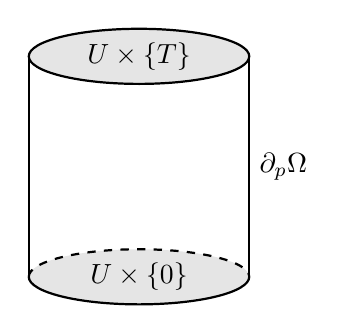
\begin{tikzpicture}[every path/.style={thick}, scale=.7]
					\fill[gray!20] (0,0) ellipse (2cm and .5cm);
					\draw (-2,0)--(-2,4);
					\draw (2,0)--(2,4);
					\filldraw[fill=gray!20] (0,4) ellipse (2cm and .5cm);
					\draw[dashed] (-2,0) arc (180:0:2cm and .5cm); 
					\draw (-2,0) arc (-180:-0:2cm and .5cm);
					\node at (0,4) {$U\times\{T\}$};
					\node at (0,0) {$U\times\{0\}$};
					\node at (2,2) [right] {$\partial_p\Omega$};
				\end{tikzpicture}
			\end{center}

			\begin{lemma}
				(Parabolic maximum principle) Let $\Omega$ be a cylinder as above. If $u\in C^2(\Omega)\cap C(\bar{\Omega})$ and $\partial_t u-\Delta u\le0$ in $\Omega$, then $\sup_\Omega u=\sup_{\partial_p\Omega}u$. In particular, if $u\le0$ on $\partial_p\Omega$ then $u\le0$ in $\Omega$. By changing $u$ to $-u$, one can also obtain a minimum principle, i.e. if $\partial_t u-\Delta u\ge0$ in $\Omega$ then $\inf_\Omega u=\inf_{\partial_p\Omega}u$.
			\end{lemma}
			\begin{proof}
				By hypothesis, $u\in C^2(U\times(0,T))$. First, let us assume that $u\in C^2(U\times(0,T])$ ($u$ is $C^2$ up to the top of $\Omega$). The function $u$ satisfies $\partial_tu-\Delta u\le0$ in $U\times (0,T]$ and $u\in C(\bar{\Omega})$. Now consider first the particular case when $\partial_tu-\Delta u<0$ in $U\times(0,T]$. Let $(x_0,t_0)$ be a point where $u$ is maximal in $\bar{\Omega}$. We will show that $(x_0,t_0)\in\partial_p\Omega$. Assume that $(x_0,t_0)\notin\partial_p\Omega$, then $(x_0,t_0)$ lies either inside $\Omega$ or at the top of $\Omega$. In both cases $x_0\in\Omega$ and $0<t_0\le T$. Since the function $x\mapsto u(x,t_0)$ in $\bar{U}$ attains the maximum at $x=x_0$, we have $\partial_{x_{j}}^2u(x_0,t_0)\le0$ for all $j=1,\dots,n$. Therefore, $\Delta u(x_0,t_0)\le0$. On the other hand, the function $t\mapsto u(x_0,t)$ in $(0,t_0]$ attains its maximum at $t=t_0$. Therefore, $\partial_t u(x_0,t_0)\ge0$.
				Hence, we conclude that $(\partial_t u-\Delta u)(x_0,t_0)\ge0$ which contradicts the assumption $\partial_tu-\Delta u<0$. Consider now the general case when $u$ satisfies $\partial_tu-\Delta u\le0$ in $U\times(0,T]$. Set $u_\epsilon:=u-\epsilon t$ with $\epsilon>0$. Clearly, $\partial_tu_\epsilon-\Delta u_\epsilon=(\partial_tu-\Delta u)-\epsilon<0$. Hence, the previous case applies to $u_\epsilon$ and we conclude that $\sup_\Omega(u-\epsilon t)=\sup_{\partial_p\Omega}(u-\epsilon t)$. Letting $\epsilon\to0$ we get $\sup_\Omega u=\sup_{\partial_p\Omega}u$. Finally, let us prove the maximum principle under the assumption that $u\in C^2(\Omega)\cap C(\bar{\Omega})$. Choose $T^\prime<T$ and consider the cylinder $\Omega^\prime=U\times(0,T^\prime)$. Then $u\in C^2(U\times(0,T^\prime])$ and, by the previous argument, we obtain that $\sup_{\Omega^\prime}u=\sup_{\partial_p\Omega}u$. Now let $T^\prime\to T$ in this equality and arrive at the desired result.
			\end{proof}

			\begin{thm}
				(Uniqueness of solution to \eqref{eq--cauchy})\\
				For any continuous function $g$ the Cauchy problem \eqref{eq--cauchy} has at most one bounded solution. 
			\end{thm}
			\begin{proof}
				Fix $T>0$ and consider the Cauchy problem
				\begin{equation*}
					\begin{cases}
						\partial_tu-\Delta u=0 & \text{on }\R^n\times(0,T)\\
						u(x,0)=0 &
					\end{cases}.
				\end{equation*}
				Then it is enough to show that any bounded set in this problem is identically equal to zero. Consider the function $v(x,t)=|x|^2+2nt$. This function is non-negative and satisfies $\partial_tv=\Delta v$. Fix $\epsilon>0$ and compare $u$ and $\epsilon v$ in a cylinder $\Omega:= B(0,R)\times B(0,T)$ where $R$ is to be chosen. At the bottom of the cylinder (i.e. $t=0$) we have $u=0
				\le\epsilon v$. At the lateral boundary of $\Omega$ (i.e. when $|x|=R$) we have $u\le\sup|u|:= C<\infty$ (since $u$ was bounded) and $v\ge R^2$, hence $\epsilon v\ge\epsilon\R^2$. Choosing $R$ so big that $\epsilon R^2\ge C$, we obtain $u\le\epsilon v$ on the lateral boundary of $\Omega$. Hence, the function $u-\epsilon v$ satisfies the heat equation in $\Omega$ and $u-\epsilon v\le0$ on $\partial_p\Omega$. So by the maximum principle $u-\epsilon v\le0$ in $\Omega$. Letting $R\to\infty$, we obtain $u-\epsilon v\le0$ in $\R^n\times(0,T)$. Letting $\epsilon\to0$, we obtain $u\le0$ in $\R^n\times(0,T)$. In the same way we can show that $u\ge0$ in $\R^n\times(0,T)$. Thus, $u\equiv0$ in $\R^n\times(0,T)$.
			\end{proof}

			\begin{remark}
				One also has the uniqueness for the Cauchy problem
				\begin{equation*}
					\begin{cases}
						\partial_tu-\Delta u=f & \text{in }U\times(0,T]=\Omega\\
						u=g & \text{on }\partial_p\Omega
					\end{cases}
				\end{equation*}
				for $f\in C(\Omega)$, $g\in C(\partial_p\Omega)$. This is a direct application of the maximum principle.
			\end{remark}

			Next we would like to establish a mean-value formula for caloric functions. 
			Let $\Omega=U\times(0,T]$ be the parabolic cylinder. Define the ``heat ball'' as follows, given $x\in\R^n$, $t\in\R$ and $r>0$. The heat ball is
			\begin{equation*}
				E(x,t;r):=\{(y,s)\in\R^{n+1}|s\le t,\,E(x-y,t-s)\ge\frac{1}{r^n}\},
			\end{equation*} 
			where $E(x,t)$ is the heat kernel, \eqref{eq--heatkernel}, of $\partial_t-\Delta$. 

			\begin{thm}
				(Mean-value property)\\
				Let $u\in C^2(\Omega)\cap C(\bar{\Omega})$ solve the heat equation. Then
				\begin{equation*}
					u(x,t)=\frac{1}{4r^n}\iint_{E(x,t;r)}u(y,s)\frac{|x-y|^2}{(t-s)^2}\,\mathrm{d}y\,\mathrm{d}s
				\end{equation*}
				for all $E(x,t;r)\subset\Omega$.
			\end{thm}
			\begin{pproof}
				See [LE] Theorem 3, p. 53.
			\end{pproof}


		\subsection{Wave Equation}

			The wave equation is given by
			\begin{equation}\label{eq--wave}
				\partial_{tt}^2u=\Delta u,
			\end{equation}
			where $u=u(x,t)$ is a function of $x\in\R^n$ and $t\in\R$. Note that the physical wave equation contains a parameter $c>0$:
			\begin{equation*}
				\partial_{tt}^2u=c^2\Delta u.
			\end{equation*}
			The parameter $c$ plays an important role as the speed of the wave as we will see below. However, the change $s=ct$ reduces the latter PDE to the former. Hence, all results with $c=1$ can be reformulated for generic $c$ using the change of time. Note also that the change $s=-t$ brings \eqref{eq--wave} to the same form, which means that the properties of the wave equation for $t>0$ and $t<0$ are the same, unlike for the heat equation.

			Let us consider the Cauchy problem for the wave equation,
			\begin{equation*}
				\begin{cases}
					\partial_{tt}^2u=\Delta u & \text{in }\R^{n+1}_+\\
					u(x,0)=g(x),\,\partial_tu(x,0)=h(x) & \text{in }\R^n
				\end{cases},
			\end{equation*}
			where $g$ and $h$ are given functions. Solutions are sought in the class $u\in C^2(\bar{\R^{n+1}_+})$. Since the method of solving the Cauchy problem depends on the dimension $n$, we consider separately the cases $n=1,2,3$.


			\subsubsection*{Cauchy Problem for $n=1$}

				Consider the Cauchy problem in the case $n=1$,
				\begin{equation}\label{eq--wave.cauchy}
					\begin{cases}
						\partial_{tt}^2u=\partial_{xx}^2u & \text{in }\R^2_+\\
						u(x,0)=g(x),\,\partial_tu(x,0)=h(x) & \text{in }\R 
					\end{cases}.
				\end{equation}
				The general $C^2$-solution of the wave equation in $\R^2$ (or in $\R^2_+$) is given by
				\begin{equation}\label{eq--linear.combination}
					u(x,t)=F(x+t)+G(x-t),
				\end{equation} 
				where $F$ and $G$ are arbitrary $C^2$-functions on $\R$. Let us find $F$ and $G$ to satisfy the initial conditions
				\begin{equation*}
					u(x,0)=g(x),\qquad \partial_tu(x,0)=h(x).
				\end{equation*}
				Indeed, substituting into the general solution for $t=0$ we immediately obtain
				\begin{equation}
					g(x)=F(x)+G(x),\qquad h(x)=F^\prime(x)-G^\prime(x).\label{eq--wave.gh}
				\end{equation}
				From this we deduce that it should be $g\in C^2$ and $h\in C^1$. Assuming this holds true, we can solve for $F$ and $G$ to obtain
				\begin{align}
					F(x)&=\frac{1}{2}\left(g(x)+\int_0^xh(y)\mathrm{d}y\right)+C,\label{eq--wave.F}\\
					G(x)&=\frac{1}{2}\left(g(x)-\int_0^xh(y)\mathrm{d}y\right)-C.\label{eq--wave.G}
				\end{align}
				We therefore obtain the following statement:

				\begin{thm}
					(D'Alembert's formula)\\
					If $g\in C^2(\R)$ and $h\in C^1(\R)$, then the following function is a unique solution of the Cauchy problem:
					\begin{equation}\label{eq--dalembert}
						u(x,t)=\frac{1}{2}\left(g(x+t)+g(x-t)\right)+\frac{1}{2}\int_{x-t}^{x+t}h(y)\mathrm{d}y.
					\end{equation}
				\end{thm}
				\begin{proof}
					The uniqueness follows from the fact that the functions $F$ and $G$ are determined uniquely, up to a constant $C$, that cancels out in \eqref{eq--linear.combination}. The function $u$ from \eqref{eq--dalembert} satisfies \eqref{eq--linear.combination}, where $F,G$ are given by \eqref{eq--wave.F} and \eqref{eq--wave.G}. It follows that $u\in C^2(\R^2)$, $u$ satisfies the wave equation in $\R^2$ and also the initial conditions by the choice of $F,G$.
				\end{proof}

				This argument shows, in addition, the following:
				\begin{enumerate}
					\item We have obtained a solution $u$ of the Cauchy problem \eqref{eq--wave.cauchy} not only in $\R^2_+$, but in all of $\R^2$.
					\item As we see from \eqref{eq--wave.gh}, the conditions $g\in C^2$ and $h\in C^1$ are not only sufficient but also necessary for $F,G\in C^2$; hence, they are also necessary for the existence of a $C^2$-solution.
				\end{enumerate}

				\begin{eg}
					Consider the initial functions
					\begin{equation*}
						g(x)=\sin x,\qquad h(x)=x.
					\end{equation*}
					Then \eqref{eq--dalembert} gives
					\begin{equation*}
						u(x,t)=\frac{1}{2}\left(\sin(x+t)+\sin(x-t)\right)+\frac{1}{4}\left((x+t)^2-(x-t)^2\right)=\sin x\cos t+xt.
					\end{equation*}
				\end{eg}

				Before we construct solutions in higher dimensions, let us discuss the uniqueness in arbitrary dimensions.

			
			\subsubsection*{Energy and Uniqueness}

				We first prove uniqueness in the setting of a mixed problem. Given a bounded region $U$ in $\R^n$ and $T>0$, consider the mixed problem for the wave equation in the cylinder $\Omega=U\times(0,T)$:
				\begin{equation}\label{eq--uniqueness}
					\begin{cases}
						\partial_{tt}^2u=\Delta u & \text{in }\Omega\\
						u=g & \text{on }\partial_p\Omega\\
						\partial_tu|_{t=0}=h & \text{in }U
					\end{cases},
				\end{equation}
				where $g$ and $h$ are given functions. Solutions $u$ are sought in $C^2(\Omega)\cap C^1(\bar{\Omega})$.

				\begin{thm}
					\phantom{k}\\ The problem \eqref{eq--uniqueness} has at most one solution in $C^2(\Omega)\cap C^1(\bar{\Omega})$.
				\end{thm}
				\begin{proof}
					It is enough to prove that, if $g=0$ and $h=0$, then $u=0$. Consider the energy of the solution $u$ at time $t$:
					\begin{equation}\label{eq--energy}
						E(t)=\frac{1}{2}\int_U((\partial_tu)^2+|\nabla u|^2)\mathrm{d}x.
					\end{equation}
					Obviously, $E(t)$  is a continuous function in $t\in[0,T]$. Differentiating $E$ in $t\in(0,T)$, we obtain
					\begin{align*}
						E^\prime(t)&=\frac{1}{2}\int_U\left(\partial_t(\partial_tu)^2+\partial_t(\nabla u\cdot\nabla u)\right)\mathrm{d}x\\
						&=\int_U(\partial_{tt}^2u\partial_tu+\nabla u\cdot\nabla\partial_tu)\mathrm{d}x.
					\end{align*}
					Now we apply Green's formula on the second term. We have $u\in C^2(U)\cap C^1(\bar{U})$ and $w:=\partial_tu\in C^1(U)\cap C(\bar{U})$. Since $u=0$ on the lateral boundary $\partial U\times[0,T]$, we obtain $w=\partial_tu=0$ on $\partial U\times[0,T]$. Hence,
					\begin{equation*}
						\int_U\nabla u\cdot\nabla\partial_tu \mathrm{d}x=-\int_U\Delta u\partial_tu \mathrm{d}x.
					\end{equation*}
					It follows that
					\begin{equation*}
						E^\prime(t)=\int_U\left(\partial_{tt}^2u\partial_tu-\Delta u\partial_tu\right)\mathrm{d}x=\int_U(\partial_{tt}^2u-\Delta u)\partial_tu \mathrm{d}x=0.
					\end{equation*}
					Therefore, $E(t)$ is constant on $[0,T]$. Since $E(0)=0$ by the initial condition $u=0$ and $\partial_tu=0$ at $t=0$, we conclude that $E(t)\equiv0$. This implies that the functions $\partial_tu$ and $|\nabla u|$ are identically equal to zero in $\Omega$, whence $u\equiv$const in $\Omega$. The initial condition $u=0$ implies $u\equiv0$ in $\Omega$, which was to be proved.
				\end{proof}

				The physical meaning of the energy \eqref{eq--energy} is the following: If $u(x,t)$ is the displacement of a vibrating membrane over $U$, then $\frac{1}{2}(\partial_tu)^2$ is (the density of) the kinetic energy at the point $x$ at time $t$, while $\frac{1}{2}|\nabla u|^2$ is (the density of) the potential energy of tension, because the latter is proportional to the increase of the area,
				\begin{equation*}
					\sqrt{1+|\nabla u|^2}-1\approx\frac{1}{2}|\nabla u|^2.
				\end{equation*}
				
				Now let us discuss uniqueness for the Cauchy problem
				\begin{equation}\label{eq--wave.cauchy.2}
					\begin{cases}
						\partial_{tt}^2u=\Delta u & \text{in }\R^n\times(0,T)\\
						u(x,0)=g(x),\,\partial_tu(x,0) & \text{in }\R^n\\ 
					\end{cases},
				\end{equation}
				where $T\in(0,\infty]$ and $u\in C^2(\R^n\times[0,T))$.

				\begin{thm}\label{thm--uniqueness}
					(Uniqueness for the Cauchy problem of the wave equation)\\ The problem \eqref{eq--wave.cauchy.2} has at most one solution $u\in C^2(\R^n\times[0,T))$.
				\end{thm}

				Note that, contrast to the case of the heat equation, there are no restrictions like boundedness of the solution.

				If $u(x,t)$ is a solution of \eqref{eq--wave.cauchy.2} then, for any open set $U\subset\R^n$ and any $t\in[0,T)$ define the energy of $u$ in $U$ at time $t$ by
				\begin{equation*}
					E_U(t)=\frac{1}{2}\int_U\left((\partial_tu)^2+|\nabla u|^2\right)\mathrm{d}x.
				\end{equation*} 
				For any $x_0\in\R^n$ and $t_0>0$, define the cone of dependence by
				\begin{equation*}
					C_{t_0}(x_0):=\{(x,t)\in\R^{n+1}|0\le t\le t_0,|x-x_0|<t_0-t\}.
				\end{equation*}

				\begin{center}
					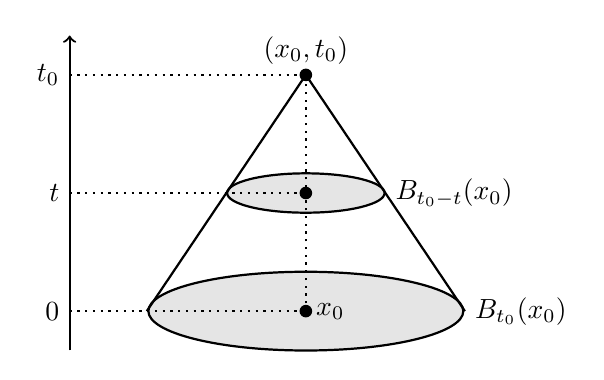
\begin{tikzpicture}[every path/.style={thick}]
						\filldraw[fill=gray!20] (0,0) ellipse (2cm and .5cm);
						\filldraw[fill=gray!20] (0,1.5) ellipse (1cm and .25cm);
						\draw (-2.02,0)--(0,3)--(2.02,0);
						\fill (0,0) circle [radius=.08cm] node [right] {$x_0$};
						\fill (0,1.5) circle [radius=.08cm];
						\node at (2.02,0) [right] {$B_{t_0}(x_0)$};
						\node at (1.01,1.5) [right] {$B_{t_0-t}(x_0)$};
						\fill (0,3) circle [radius=.08cm] node [above] {$(x_0,t_0)$};
						\draw[dotted] (0,0)--(0,3);
						\draw[->] (-3,-.5)--(-3,3.5);
						\node at (-3,0) [left] {$0$};
						\node at (-3,1.5) [left] {$t$};
						\node at (-3,3) [left] {$t_0$};
						\draw[dotted] (-3,1.5)--(0,1.5);
						\draw[dotted] (-3,3)--(0,3);
						\draw[dotted] (-3,0)--(0,0);
					\end{tikzpicture}
				\end{center}

				Clearly, at each level $t\in[0,t_0]$, the cone $C_{t_0}(x_0)$ consists of the closed ball $\bar{B_{t_0-t}(x_0)}$. In particular, the base of the cone at $t=0$ is the ball $\bar{B_{t_0}(x_0)}$, the top of the cone at $t=t_0$ is the point $x_0$.

				The following theorem plays the main role in the proof of \autoref{thm--uniqueness}:

				\begin{thm}\label{thm--wave}
					(Domain of dependence)\\
					If $u\in C^2(C_{t_0}(x_0))$ is a solution of the wave equation in $C_{t_0}(x_0)$ and $u(x,0)=0$ and $\partial_t u(x,0)=0$, then $u\equiv0$ in $C_{t_0}(x_0)$.
				\end{thm}
                \begin{proof}
					(of \autoref{thm--uniqueness}) It is enough to prove that, if $g=0$ and $h=0$, then $u=0$. Choose any point $x_0\in\R^n$ and $t_0\in(0,T)$. Since $g=h=0$ in $B_{t_0}(x_0)$, we obtain by \autoref{thm--wave} that $u=0$ in the cone $C_{t_0}(x_0)$ and, in particular, at $(x_0,t_0)$. Since $(x_0,t_0)$ is arbitrary, we obtain $u\equiv0$, which was to be proved.
				\end{proof}

				\begin{proof}(of \autoref{thm--wave})
					For simplicity of notation take $x_0=0$ and skip $x_0$ from all notations. Now consider the energy of $u$ in the ball $B_{t_0-t}$ at time $t$,
					\begin{equation*}
						F(t):=E_{B(t_0-t)}(t)=\frac{1}{2}\int_{B_{t_0-t}}\left((\partial_t u)^2+|\nabla_x u|^2\right)\mathrm{d}x.
					\end{equation*}
					$F$ is continuous in $[0,t_0]$. By hypothesis, $F(0)=0$. Let us show that $F^\prime(t)\le0$ for $t\in[0,t_0]$ which will then imply that $F(t)\equiv0$ in $[0,t_0]$. In turn, this will yield that $\partial_t u=0$ and $\nabla u=0$ in $C_{t_0}$, that is, $u$ is constant in $C_{t_0}$. Whence $u\equiv0$ in $C_{t_0}$ as desired. In order to differentiate $F$, let us first consider the simpler function
					\begin{equation*}
						\Phi(r,t):=E_{B_r}(t)=\frac{1}{2}\int_{B_r}\left((\partial_t u)^2+|\nabla_x u|^2\right)\mathrm{d}x
					\end{equation*}
					is defined wherever $\bar{B_r}\times\{t\}$ lies in the domain of $u$. As we saw before,
					\begin{align*}
						\partial_t\Phi&=\frac{1}{2}\int_{B_r}\partial_t\left((\partial_t u)^2+\nabla u\cdot\nabla u\right)\mathrm{d}x\\
						&=\int_{B_r}\left(\partial_{tt}^2u\partial_t u+\nabla_x u\nabla_x\partial_t u\right)\mathrm{d}x\\
						&=\int_{B_r}\left(\partial_{tt}^2-\Delta u\right)\partial_t u\mathrm{d}x+\int_{\partial B_r}\partial_\nu u\partial_t u \mathrm{d}\sigma\\
						&=\int_{\partial B_r}\partial_\nu u\partial_t u \mathrm{d}\sigma
					\end{align*}
					since $u$ satisfies the wave equation. As $\partial_\nu u\partial_t u\le|\nabla u||\partial_t u|\le\frac{1}{2}\left((\partial_tu)^2+|\nabla u|^2\right)$ we obtain
					\begin{equation*}
						\partial_t\Phi\le\frac{1}{2}\int_{\partial B_r}\left((\partial_tu)^2+|\nabla u|^2\right)\mathrm{d}\sigma.
					\end{equation*}
					Next, represent the integral over the ball $B_r$ as a repeated integral over the radius and over the spheres:
					\begin{equation*}
						\partial_r\Phi=\frac{1}{2}\frac{\partial}{\partial r}\int_0^r\left(\int_{\partial B_s}\left((\partial_t u)^2+|\nabla u|^2\right)\mathrm{d}\sigma\right)\mathrm{d}s=\frac{1}{2}\int_{\partial B_r}\left((\partial_t u)^2+|\nabla_xu|^2\right)\mathrm{d}\sigma\ge\partial_t\Phi.
					\end{equation*}
					Now we can differentiate the equation $F(t)=E_{B_{t_0-t}}(t)=\Phi(t_0-t,t)$. The chain rule yields
					\begin{equation*}
						F^\prime(t)=-\partial_r\Phi(t_0-t,t)+\partial_t\Phi(t_0-t,t)\le0
					\end{equation*}
					by the previous estimate.
				\end{proof}

				\begin{cor}
					(Finite propagation speed) Let $u\in C^2(\R^n\times[0,T))$ be a solution to the wave equation in $\R^n\times(0,T)$. If for some $R>0$, $\supp u(x,0)\subset\bar{B_R}$ and $\supp\partial_tu(x,0)\subset\bar{B_R}$, then for any $0<t<T$, $\supp u(x,t)\subset \bar{B_{R+T}}$.
				\end{cor}

				\noindent\underline{NB}: This shows that the wave travels in time $t$ a distance of at most $t$ (or, more accurately, $c\cdot t$), that is the speed of propagation is bounded by 1 (or $c$).

				\begin{proof}
					Fix some $t_0\in(0,T)$ and a point $x_0\notin\bar{B_{R+t_0}}$. Then it is enough to show that $u(x_0,t_0)=0$. Indeed, the cone $C_{t_0}(x_0)$ is based on the ball $\bar{B_{t_0}(x_0)}$ and due to the condition $x_0\notin\bar{B_{R+t_0}}$ we see that the balls $\bar{B_{t_0(x_0)}}$ and $\bar{B_R}$ are disjoint. Therefore, $u$ and $\partial_t u$ vanish at $t=0$ in $\bar{B_{t_0}(x_0)}$. By \autoref{thm--wave}, $u\equiv0$ in $C_{t_0}(x_0)$, therefore in particular we have that $u(x_0,t_0)=0$.
			\end{proof}		
					
					Now let us see what the Fourier transform can achieve for the Cauchy problem for the wave equation.
					Using the Fourier transform one can solve the wave equation in the following way:
					\begin{equation*}
						\begin{cases}
							\partial_{tt}^2u=\Delta u\\
							u(x,0)=f(x)\\
							\partial_tu(x,0)=g(x)
						\end{cases}\quad\overset{\text{Fourier transform}}{\Longrightarrow}\quad
						\begin{cases}
							\partial_{tt}^2\hat{u}(\xi,t)=-|\xi|^2\hat{u}(\xi,t)\\
							\hat{u}(\xi,0)=\hat{f}(\xi)\\
							\partial_t\hat{u}(\xi,0)=\hat{g}(\xi)
						\end{cases}.
					\end{equation*}
					Note that we have a simple ODE on the right hand side now which we can solve as follows: make an ansatz $\hat{u}(\xi,t)=A(\xi)\cos(t|\xi|)+B(\xi)\sin(t|\xi|)$ with $\hat{u}(\xi,0)=A(\xi)=\hat{f}(\xi)$. We have
					\begin{equation*}
						\partial_t\hat{u}=-A(\xi)|\xi|\sin(t|\xi|)+B(\xi)|\xi|\cos(t|\xi|)
					\end{equation*}
					and get $\partial_t\hat{u}(\xi,0)=B(\xi)|\xi|=\hat{g}(\xi)$. Thus, the solution is given by
					\begin{equation*}
						\hat{u}(\xi,t)=\hat{f}(\xi)\cos(t|\xi|)+\frac{\hat{g}(\xi)}{|\xi|}\sin(t|\xi|)
					\end{equation*}
					and
					\begin{equation*}
						u(x,t)=\F^{-1}\left(\hat{f}(\xi)\cos(t|\xi|)+\frac{\hat{g}(\xi)}{|\xi|}\sin(t|\xi|)\right)(x).
					\end{equation*}
					Note that there is no universal formula for the (inverse) Fourier transform of $\cos(t|\xi|)$ and $\frac{\sin(t|\xi|)}{|\xi|}$ in all dimensions.
			

				\noindent\underline{NB}: Although spelling out the inverse Fourier tranform in the proof is hard, just using $\hat{u}(\xi,t)$ is still good enough to estimate solutions $u(x,t)$, e.g. in $L^2$ using the Plancherel formula, \autoref{rem--plancherel}. Indeed, we have that
				\begin{equation*}
					\norm{u(t, \cdot)}_{L^2_{x}}\le\|\hat{f}\cos(t|\cdot|)\|_{L^2}+
				\|\hat{g}\,\frac{\sin(t|\cdot|)}{|\cdot|}\|_{L^2}\le\|\hat{f}\|_{L^2}+\norm{\hat{g}}_{L^2}\le\norm{f}_{L^2}+\norm{g}_{L^2},
				\end{equation*}
                which means that, for fixed time $t$, $L^2$-Cauchy data yield a solution that is spatially in $L^2(\mathbb{R}^n).$

			\subsubsection*{Cauchy Problem for the Wave Equation in Two and Three Dimensions}

				\begin{defi}(Spherical mean)
					Given a continuous function $f\in\R^n$, fix $x\in\R^n$ and define for any $r>0$ the function 
					\begin{equation}\label{eq--sphericalmean}
						F(x,r)=\dashint_{\partial B_r(x)}f(y)\mathrm{d}\sigma(y)=\frac{1}{\omega_nr^{n-1}}\int_{\partial B_r(x)}f(y)\mathrm{d}\sigma(y),
					\end{equation}
					where $\omega_n$ is the surface measure of $S^{n-1}$. The function $F(x,r)$ is called the spherical mean of $f$. When $x$ is fixed, then we use the simpler notation $F(r)$ instead of $F(x,r)$.
				\end{defi}

				\begin{lemma}\label{lem--sphericalmean}
					Fix $x\in\R^n$. If $f\in C^m(\R^n)$ where $m\ge0$, then $F\in C^m([0,\infty))$. Furthermore, if $f\in C^2(\R^n)$ then for all $r>0$,
					\begin{equation}\label{eq--sphericalmean2}
						F^\prime(r)=\dashint_{\partial B_r(x)}\partial_\nu f(y)\mathrm{d}\sigma(y)=\frac{r}{n}\dashint_{B_r(x)}\Delta f(y)\mathrm{d}y,
					\end{equation}
					where $\nu$ is the outer unit normal vector field on $\partial B_r(x)$ and
					\begin{equation}\label{eq--sphericalmean3}
						F^{\prime\prime}(r)=\dashint_{\partial B_r(x)}\Delta f(y)\mathrm{d}\sigma(y)-\frac{n-1}{n}\dashint_{B_r(x)}\Delta f(y)\mathrm{d}y.
					\end{equation} 
					For $r=0$ we have $F(0)=f(x)$, $F^\prime(0)=0$ and $F^{\prime\prime}=\Delta f/n$.
				\end{lemma}
				\begin{proof}
					Make a change of variables, $y=x+rz$ in \eqref{eq--sphericalmean} observing that $y\in\partial B_r(x)\Longleftrightarrow$ $z\in\partial B_1(0)$ and $\mathrm{d}\sigma(y)=r^{n-1}\mathrm{d}\sigma(z)$ yields
					\begin{equation*}
						F(r)=\frac{1}{\omega_nr^{n-1}}\int_{\partial B_r(x)}f(y)\mathrm{d}\sigma(y)=\frac{1}{\omega_n}\int_{\partial B_1(0)}f(x+rz)\mathrm{d}\sigma(z).
					\end{equation*}
					From this we see that $F$ is well-defined for all $r\ge0$ (in fact for all $r\in\R$). Moreover, if $f\in C^m(\R^n)$ then $F\in C^m([0,\infty))$. Let us now assume that $f\in C^2(\R^n)$, then differentiating the expression above in $r$ for $r>0$, we obtain 
					\begin{align*}
						F^\prime(r)&=\frac{1}{\omega_n}\int_{\partial B_1(0)}\partial_rf(x+rz)\mathrm{d}\sigma(z)\\
						&=\frac{1}{\omega_n}\int_{\partial B_1(0)}(\nabla f)(x+rz)\cdot z\mathrm{d}\sigma(z)\\
						&=\frac{1}{\omega_nr^{n-1}}\int_{\partial B_r(x)}(\nabla f)(y)\cdot\frac{y-x}{r}\mathrm{d}\sigma(y).
					\end{align*}
					Since $(x-y)/r=\nu$ is the outer unit normal vector field on $\partial B_r(x)$, we obtain that 
					\begin{equation*}
						(\nabla f)(y)\cdot\frac{y-x}{r}=\nabla f\cdot\nu=\partial_\nu f.
					\end{equation*}
					Therefore,
					\begin{equation*}
						F^\prime(r)=\frac{1}{\omega_nr^{n-1}}\int_{\partial B_r(x)}\partial_\nu f\mathrm{d}\sigma=\dashint_{\partial B_r(x)}\partial_\nu f(y)\mathrm{d}\sigma(y),
					\end{equation*}
					which is the first equality in \eqref{eq--sphericalmean2}. Next, Green's formula yields
					\begin{align*}
						F^\prime(r)&=\frac{1}{\omega_nr^{n-1}}\int_{\partial B_r(x)}\partial_\nu f(y)\mathrm{d}\sigma(y)\\
						&=\frac{1}{\omega_nr^{n-1}}\int_{B_r(x)}\Delta f(y)\mathrm{d}y\\
						&=\frac{r}{n}\frac{1}{\omega_n\frac{r^n}{n}}\int_{B_r(x)}\Delta f(y)\mathrm{d}y\\
						&=\frac{r}{n}\dashint_{B_r(x)}\Delta f(y)\mathrm{d}y,
					\end{align*}
					which shows the second equality in \eqref{eq--sphericalmean2}. Rewrite the latter equality in the form $F^\prime(r)=\frac{1}{\omega_nr^{n-1}}G(r)$, where
					\begin{equation*}
						G(r)=\int_{\partial B_r(x)}\Delta f(y)\mathrm{d}y=\int_0^r\left(\int_{\partial_s B(x)}\Delta f(y)\mathrm{d}\sigma(y)\right)\mathrm{d}s,
					\end{equation*}
					we see that $G$ is differentiable in $r$ and
					\begin{equation*}
						G^\prime(r)=\int_{\partial B_r(x)}\Delta f(y)\mathrm{d}\sigma(y)
					\end{equation*}
					by the fundamental theorem of calculus. Thus,
					\begin{align*}
						F^{\prime\prime}&=\frac{\mathrm{d}}{\mathrm{d}r}\left(\frac{1}{\omega_nr^{n-1}}G(r)\right)\\
						&=\frac{1}{\omega_nr^{n-1}}G^\prime(r)-\frac{n-1}{\omega_nr^n}G(r)\\
						&=\frac{1}{\omega_nr^{n-1}}\int_{\partial B_r(x)}\Delta f(y)\mathrm{d}\sigma(y)-\frac{n-1}{\omega_nr^n}\int_{B_r(x)}\Delta f(y)\mathrm{d}y\\
						&=\dashint_{\partial B_r(x)}\Delta f(y)\mathrm{d}\sigma(y)-\frac{n-1}{n}\dashint_{B_r(x)}\Delta f(y)\mathrm{d}y,
					\end{align*}
					which proves \eqref{eq--sphericalmean3}. Finally, take limits in \eqref{eq--sphericalmean}, \eqref{eq--sphericalmean2} and \eqref{eq--sphericalmean3} where $r\to0$ and using the continuity of $f$ and of $\nabla f$ we obtain what is claimed.
				\end{proof}

				\begin{lemma}
					If $f\in C^m(\R^n)$, then $F$ as a function of $(x,r)$ belongs to $C^m(\R^n\times[0,\infty))$. If $f\in C^2(\R^n)$, then for any $r\ge0$,
					\begin{equation*}
						\Delta F(x,r)=\dashint_{\partial B_r(x)}\Delta f(y)\mathrm{d}y.
					\end{equation*}
				\end{lemma}
				\begin{proof}
					Recall that $F(x,r)=\frac{1}{\omega_n}\int_{\partial B_1(0)}f(x+rz)\mathrm{d}\sigma(z)$. Hence, using $\Delta_x(f(x+rz))=(\Delta f)(x+rz)$ the lemma follows immediately.
				\end{proof}

				Now let us consider the Cauchy problem
				\begin{equation*}
					\begin{cases}
						\partial_{tt}^2u=\Delta u & \text{in }\R^{n+1}_+\\
						u(x,0)=g(x),\,\partial_tu(x,0)=h(x) & \text{in }\R^n
					\end{cases}.
				\end{equation*}
				The functions $g$ and $h$ are assumed as given (the so-called Cauchy data). We will assume that $u\in C^2(\bar{\R^{n+1}_+})$ and $g\in C^2(\R^n)$, $h\in C^1(\R^n)$. Assuming that the solution exists, we would like to deduce a formula for it in terms of $g$ and $h$. Define 
				\begin{equation*}
					G(x,r):=\dashint_{\partial B_r(x)}g(y)\mathrm{d}\sigma(y),\,\, H(x,r):=\dashint_{\partial B_r(x)}h(y)\mathrm{d}\sigma(y),\,\, U(x,r,t):=\dashint_{\partial B_r(x)}u(y,t)\mathrm{d}\sigma(y),
				\end{equation*}
				for $x\in\R^n$ and $r>0$. All these functions are also defined for $r=0$ by continuity. Suppress $x$ in the notation (for now). Also set $Q:=\R_+\times(0,\infty)$ and denote the points of $Q$ by $(r,t)$ with $r,t>0$. Then the following proposition holds:

				\begin{prop}
					(Euler-Poisson-Darboux equation, Leonhard Euler Swiss mathematician and physicist and Gaston Darboux French mathematician) If $u$ solves the Cauchy problem for the wave equation, then for any $x\in\R^n$, the function $U(r,t)$ belongs to $C^2(Q)$ and solves the Euler-Poisson-Darboux equation 
					\begin{equation*}
						\begin{cases}
							\partial_{tt}^2U=\partial_{rr}^2U+\frac{n-1}{r}\partial_r U & \text{in }Q\\
							U(0,t)=u(x,t) & \text{for all }t\ge0\\
							U(r,0)=G(r),\,\partial_t U(r,0)=H(r) & \text{for all }r\ge0
						\end{cases}
					\end{equation*}
					which is a PDE in 1+1 variables.
				\end{prop}
				\begin{proof}
					By the definition of $U(r,t)$ we have
					\begin{equation*}
						U(r,t)=\frac{1}{\omega_n}\int_{\partial B_1(0)}u(x+rz,t)\mathrm{d}\sigma(z)
					\end{equation*}
					which implies that $U\in C^2(\bar{Q})$. We know by \autoref{lem--sphericalmean} that
					\begin{equation*}
						\partial_rU=\frac{r}{n}\dashint_{B_r(x)}\Delta u(y,t)\mathrm{d}y
					\end{equation*}
					and by \eqref{eq--sphericalmean3} we have
					\begin{equation*}
						\partial_{rr}^2U=\dashint_{\partial B_r(x)}\Delta u(y,t)\mathrm{d}\sigma(y)-\frac{n-1}{n}\dashint_{B_r(x)}\Delta u(y,t)\mathrm{d}y
					\end{equation*}
					which yields
					\begin{equation*}
						\partial_{rr}^2U+\frac{n-1}{r}\partial_rU=\dashint_{\partial B_r(x)}\Delta u(y,t)\mathrm{d}\sigma(y)\overset{\text{wave eq.}}{=}\dashint_{\partial B_r(x)}\partial_{tt}^2u(y,t)\mathrm{d}\sigma(y)=\partial_{tt}^2U.
					\end{equation*}
					The boundary condition is $U(0,t)=u(x,t)$ and the rest follows similarly from $u(x,0)=g(x)$ and $\partial_tu(x,0)=h(x)$.
				\end{proof}


				Consider the Cauchy problem for the three-dimensional wave equation,
				\begin{equation}\label{eq--wave3d}
					\begin{cases}
						\partial_{tt}^2u=\Delta u & \text{in }\R^{3+1}_+\\
						u(x,0)=g(x),\,\partial_tu(x,0)=h(x) & \text{in }\R^3
					\end{cases}.
				\end{equation}
				We seek a solution $u\in C^2(\bar{\R^{3+1}_+})$ with $g\in C^2(\R^3)$ and $h\in C^1(\R^3)$.

				\begin{thm}
					(Kirchhoff, after German physicist Gustav Kirchoff)\\
					If $u$ is a solution of \eqref{eq--wave3d}, then for all $x\in\R^3$ and $t>0$,
					\begin{equation*}
						u(x,t)=\dashint_{\partial B_t(x)}\left(g(y)+t\partial_\nu g(y)+th(y)\right)\mathrm{d}\sigma(y).
					\end{equation*}
				\end{thm}

				\begin{remark}({\bf{Huygens' principle}})
					The ball $\bar{B_t(x)}$ is the bottom of the cone of dependence $C_t(x)$. As we have seen earlier, the value of $u(x,t)$ is completely determined by the initial conditions in the ball $\bar{B_t(x)}$. Kirchhoff's theorem shows that in dimension three a stronger statement holds, namely $u(x,t)$ is completely determined by the initial conditions on the sphere $\partial B_t(x)$, as opposed to the one-dimensional problem. This phenomenon was discovered for the first time by the Dutch mathematician and physicist Christiaan Huygens and is called Huygens' principle.
				\end{remark}

				\begin{proof}
					We use the spherical means $U,G,H$. Consider also the functions $\tilde{U}:=rU$, $\tilde{G}:=rG$ and $\tilde{H}:=rH$. Now using the Euler-Poisson-Darboux equations with $n=3$ we obtain
					\begin{equation*}
						\partial_{rr}^2\tilde{U}=\partial_{rr}^2U+2\partial_rU=\partial_{tt}^2\tilde{U}.
					\end{equation*}
					Therefore, $\tilde{U}\in C^2(Q)$ where $Q=\R_+\times(0,\infty)$ and $\tilde{U}$ solves the problem 
					\begin{equation*}
						\begin{cases}
							\partial_{tt}^2\tilde{U}=\partial_{rr}\tilde{U} & \text{in }Q\\
							\tilde{U}(0,t)=0 & \text{for all }t\ge0\\
							\tilde{U(r,0)}=\tilde{G}(r) & \text{for all }r\ge0\\
							\partial_t\tilde{U}(r,0)=\tilde{H}(r) & \text{for all }r\ge0
						\end{cases}.
					\end{equation*}
					Now since $\tilde{U}$ is a solution of the wave equation in one dimension in $Q$, it has to be of the form
					$\tilde{U}=\Phi(r+t)+\Psi(r-t)$ for some $C^2$-functions $\Phi$, $\Psi$ in $\R$. To determine $\Phi$ and $\Psi$, setting $r=0$ and $\tilde{U}(0,t)=0$ we get $\Phi(t)=-\Psi(-t)$ for all $t\ge0$. Setting $t=0$ we get $\Phi(r)+\Psi(r)=\tilde{G}(r)$. Differentiating $\tilde{U}$ in $t$ and setting $t=0$ we obtain $\Phi^\prime(r)-\Psi^\prime(r)=\tilde{H}(r)$,
					\begin{equation*}
						\Phi(r)=\frac{1}{2}\left(\tilde{G}(r)+\int_0^r\tilde{H}(s)\mathrm{d}s\right),\qquad \Psi(r)=\frac{1}{2}\left(\tilde{G}(r)-\int_0^r\tilde{H}(s)\mathrm{d}s\right).
					\end{equation*}
					In the range $0\le r\le t$ we have
					\begin{align*}
						\tilde{U}(r,t)=&\Phi(r+t)+\Psi(r-t)\\
						=&\Phi(r+t)-\Phi(t-r)\\
						=&\frac{1}{2}\left(\tilde{G}(r+t)-\tilde{G}(t-r)\right)+\frac{1}{2}\int_{t-r}^{t+r}\tilde{H}(s)\mathrm{d}s.
					\end{align*}
					Since
					$u(x,t)=\lim_{r\to0}U(x,r,t)=\lim_{r\to0}\frac{\tilde{U}(x,r,t)}{r}$ it follows that
					\begin{equation*}
						u(x,t)=\lim_{r\to0}\left(\frac{\tilde{G}(t+r)-\tilde{G}(t-r)}{2r}+\frac{1}{2r}\int_{t-r}^{t+r}\tilde{H}(s)\mathrm{d}s\right)=G+tG^\prime+tH.
					\end{equation*} 
					By a previous lemma, $G^\prime(t)=\dashint_{\partial_t(x)}\partial_\nu g(y)\mathrm{d}\sigma(y)$, so Kirchhoff's formula follows. Conversely, one can show that if $g\in C^3(\R^3)$ and $h\in C^2(\R^3)$, then the function 
					\begin{equation*}
						u(x,t)=\dashint_{\partial B_t(x)}\left(g(y)+t\partial_\nu g(t)+th(y)\right)\mathrm{d}\sigma(y).
					\end{equation*}
					Indeed, the previous proof shows that $u=\partial_t(tG)+tH=G+t\partial_tG+tH$ and by a previous lemma we have that $G\in C^3$ and $H\in C^2$, whence $u\in C^3(\R^3\times[0,\infty))$. At $t=0$ we obtain $u(x,0)=G(x,0)=g(x)$. Since $\partial_tu=2\partial_tG+t\partial_{tt}^2G+t\partial_tH+H$ it follows that $\partial_tu(x,0)=H(x,0)=h(x)$. To verify that $u$ satisfies the wave equation it is enough to show that each of the functions do. Consider first the function $v(x,t)=tH(x,t)$. We have that
					\begin{align*}
						\partial_{tt}^2v&=2\partial_tH+t\partial_{tt}^2H\\
						&=\frac{2t}{3}\dashint_{B_t(x)}\Delta h \mathrm{d}y+t\dashint_{\partial B_t(x)}\Delta h \mathrm{d}\sigma(y)-\frac{2}{3}t\dashint_{B_t(x)}\Delta h \mathrm{d}y\\
						&=t\dashint_{\partial B_t(x)}\Delta h \mathrm{d}\sigma(y)\\
						&=t\Delta H\\
						&=\Delta v.
					\end{align*}
					So $v$ satisfies the wave equation. Since $w=tG$ satisfies the wave equation $\partial_{tt}^2w=\Delta w$, differentiating this equation in $t$ and noticing that $\partial_t$ commutes with $\partial_{tt}^2$ and $\Delta$, we obtain that $\partial_tw$ also satisfies the wave equation.
				\end{proof}

				Finally, consider the two-dimensional wave equation
				\begin{equation}\label{eq--wave2d}
					\begin{cases}
						\partial_{tt}^2u=\Delta u & \text{in }\R^{2+1}_+\\
						u(x,0)=g(x),\,\partial_tu(x,0)=h(x) & \text{in }\R^2
					\end{cases}. 
				\end{equation}
				We seek a solution $u\in C^2(\bar{\R^{2+1}_+})$.

				\begin{thm}
					(Poisson)\\
					Let $g\in C^3(\R^2)$ and $h\in C^2(\R^2)$. Then \eqref{eq--wave2d} has the following solution:
					\begin{equation*}
						u(x,t)=\frac{1}{2}\dashint_{B_t(x)}\frac{tg(y)+t\nabla g\cdot(y-x)+t^2h(y)}{\sqrt{t^2-|x-y|^2}}\mathrm{d}y.
					\end{equation*}
				\end{thm}
				\begin{proof}
					Let us extend \eqref{eq--wave2d} to \eqref{eq--wave3d} by the following trick: Any function $f(x_1,x_2)$ defined in $\R^2$ extends trivially to a function in $\R^3$, simply by setting $f(x_1,x_2,x_3)=f(x_1,x_2)$. So extend $u,g,h$ to $\R^3$ in this way. In particular, $u(x_1,x_2,x_3,t)=u(x_1,x_2,t)$ and $\partial_{x_1x_1}^2u+\partial_{x_2x_2}^2u+\partial_{x_3x_3}^2u=\partial_{x_1x_1}^2u+\partial_{x_2x_2}^2u$. Hence, \eqref{eq--wave2d} is equivalent to the following \eqref{eq--wave3d} problem:
					\begin{equation*}
						\begin{cases}
							\partial_{tt}^2u=\Delta u & \text{in }\R^{3+1}_+\\
							u(x,0)=g(x),\,\partial_tu(x,0)=h(x) & \text{in }\R^3
						\end{cases}
					\end{equation*}
					and an additional condition is that $U$ should not depend on $x_3$. Denote points in $\R^3$ by $X=(x_1,x_2,x_3)$ and points in $\R^2$ by $x=(x_1,x_2)$. Now by Kirchhoff's formula one has
					\begin{equation*}
						u(X,t)=\dashint_{\partial B_t(X)}\left(g+t\partial_\nu g+th\right)\mathrm{d}\sigma.
					\end{equation*} 
					Using the fact that $g$ and $h$ do not depend on $x_3$, we shall try to transform the Kirchhoff formula above to contain integration only in $\R^2$, and at the same time we check that $u$ does not depend on $x_3$. Note that the sphere $\partial B_t(X)$ is given by
					\begin{equation*}
						(y_1-x_1)^2+(y_2-x_2)^2+(y_3-x_3)^2=t^2
					\end{equation*}
					and it consists of two hemispheres which can be represented by the graphs of the functions $y_3=x_3\pm\sqrt{t^2-(y_1-x_1)^2-(y_2-x_2)^2}$ over the disk $D_t(x)$ in $\R^2$ of radius $t$ centered at $x$. If a surface $S$ in $\R^3$ is given by a graph $y_3=f(y)$, $y\in\Omega$ with $\Omega\subset\R^2$, for any continuous function $\Phi$ on $S$,
					\begin{equation}\label{eq--surfaceint}
						\int_S\Phi(Y)\mathrm{d}\sigma(Y)=\int_{\Omega}\Phi(y,f(y))\sqrt{1+|\nabla f(y)|^2}\mathrm{d}y.
					\end{equation}
					In our case, $S$ is one of the hemispheres of $\partial B_t(X)$ and $\Omega=D_t(x)$, $f(y)=x_3+\sqrt{t^2-|x-y|^2}$ and $\Phi=y+t\partial_\nu g+th$. Observe that $\partial_{x_3}g=0$ and at any point $Y\in\partial B_t(X)$ the normal vector $\nu$ is given by $\nu=\frac{Y-X}{t}$. Thus, $t\partial_\nu g=t\nabla g\cdot\frac{Y-X}{t}=\nabla g\cdot(y-x)$. Since $g$ and $h$ depend only on $y$, we obtain $\Phi(y)=g(y)+\nabla g\cdot(y-x)+th(y)$. In particular, $\Phi$ does not depend on $y_3$ and so in the expression $\Phi(Y)=\Phi(y,f(y))$ we do not have to substitute the value of $f(y)$. For $j=1,2$ we have $\partial_{y_j}f=\pm\frac{y_j-x_j}{\sqrt{t^2-|y-x|^2}}$, whence $1+|\nabla f|^2=\frac{t^2}{t^2-|y-x|^2}$. Plugging this into the surface integral \eqref{eq--surfaceint} yields
					\begin{equation*}
						\int_S\Phi(Y)\mathrm{d}\sigma(Y)=\int_{D_t(x)}\frac{tg(y)+t\nabla g\cdot(y-x)+t^2h(y)}{\sqrt{t^2-|x-y|^2}}\mathrm{d}y.
					\end{equation*}
					Finally, we obtain
					\begin{align*}
						u(X,t)&=\frac{2}{4\pi t^2}\int_{D_t(x)}\frac{tg(y)+t\nabla g\cdot(y-x)+t^2h(y)}{\sqrt{t^2-|x-y|^2}}\mathrm{d}y\\
						&=\frac{1}{2}\dashint_{D_t(x)}\frac{tg(y)+t\nabla g\cdot(y-x)+t^2h(y)}{\sqrt{t^2-|x-y|^2}}\mathrm{d}y
					\end{align*}
					and here we see that the right-hand side does not depend on $x_3$.
				\end{proof}

				\begin{remark}
					One has similar formulas for the solution of the Cauchy problem in even and odd dimensions for the wave equation (see [LE] pages 74-79).
				\end{remark}



\end{document}